\documentclass{report}

\usepackage{tabulary}

\usepackage{booktabs}
\usepackage{listings}
\usepackage{xcolor}
\usepackage{adjustbox}
\usepackage{rotating}
\usepackage{amsmath} 
\usepackage{mathtools}
\usepackage[toc,page]{appendix}
% Load the package with the acronym option
\usepackage[acronym,nomain]{glossaries}
\usepackage{setspace}
\usepackage{fancyhdr}
\usepackage{hyperref}
\usepackage[utf8]{inputenc}
\usepackage {graphicx}
\usepackage{array}
\usepackage{lastpage}
\usepackage[hmargin=2cm,top=4cm,headheight=65pt,footskip=65pt]{geometry}

\hypersetup{
	colorlinks=true,
	linkcolor=blue,
	filecolor=magenta,      
	urlcolor=cyan,
}
\setlength{\parindent}{0.95cm}
\pagestyle{fancy}
%section change begin in 0 to begin in 1
\renewcommand{\thesection}{\arabic{section}}

\renewcommand{\headrulewidth}{0pt}
\makeatletter
\renewcommand{\maketitle}{
	\noindent
		%%{\huge  \bf \href{https://www.pst.ag/}{PST, AG} }  \newline 
		%%{\footnotesize Frauentorstraße 3} \newline
		{\footnotesize Maracay, Venezuela} \newline
		%%D - 99423 Weimar \hfill \newline
	 .{\Large \hfill Ellaborated in January, 2016}//

\begin{center}
\pagestyle{empty}
\phantom{.}  %necessary to add space on top before the title
\vspace{3cm}

{\Huge \bf \@title\par}
\vspace{2.5cm}
{\LARGE Luis Ramos}\\[1cm]
\vspace{4.5cm}

%if you want something in the bottom of the page just use /vfill before that.
{ Document Version: 0.1}   \\[1cm] 

\end{center}

}\makeatother



%define json formatting

\colorlet{punct}{red!60!black}
\definecolor{background}{HTML}{EEEEEE}
\definecolor{delim}{RGB}{20,105,176}
\colorlet{numb}{magenta!60!black}

\lstdefinelanguage{json}{
	basicstyle=\normalfont\ttfamily,
	numbers=left,
	numberstyle=\scriptsize,
	stepnumber=1,
	numbersep=8pt,
	showstringspaces=false,
	breaklines=true,
	frame=lines,
	backgroundcolor=\color{background},
	literate=
	*{0}{{{\color{numb}0}}}{1}
	{1}{{{\color{numb}1}}}{1}
	{2}{{{\color{numb}2}}}{1}
	{3}{{{\color{numb}3}}}{1}
	{4}{{{\color{numb}4}}}{1}
	{5}{{{\color{numb}5}}}{1}
	{6}{{{\color{numb}6}}}{1}
	{7}{{{\color{numb}7}}}{1}
	{8}{{{\color{numb}8}}}{1}
	{9}{{{\color{numb}9}}}{1}
	{:}{{{\color{punct}{:}}}}{1}
	{,}{{{\color{punct}{,}}}}{1}
	{\{}{{{\color{delim}{\{}}}}{1}
	{\}}{{{\color{delim}{\}}}}}{1}
	{[}{{{\color{delim}{[}}}}{1}
	{]}{{{\color{delim}{]}}}}{1},
}



\title{Onto\textit{Smart} Applied in the Manufacturing Domain}  % you can actually insert these directly above if you prefer.
\date{\today}


%insert header figure
\setlength\headheight{26pt} 

%%\rhead{
\includegraphics[width=3cm]{pst_header.png}}

%\lhead{Page \thepage}
%\rfoot{Page \thepage}
%\lfoot{Page \thepage}
% Generate the glossary

\makeglossaries
\loadglsentries{myglossary}
\bibliographystyle{plain}
\begin{document}
    \maketitle
    \tableofcontents
    \section{Changes}
\begin{tabular}{|m{3.0cm}|m{6.0cm}|m{6.0cm}|}
	\hline
	\textbf{Date} & \textbf{Author} & \textbf{Description}
	\tabularnewline
	\hline
	\today  & Luis Ramos &
	Initial implementation of Onto\textit{Smart}
	\tabularnewline
	\hline & &
	\tabularnewline
	\hline
\end{tabular}
    \section{Changes}
\begin{tabular}{|m{3.0cm}|m{6.0cm}|m{6.0cm}|}
	\hline
	\textbf{Date} & \textbf{Author} & \textbf{Description}
	\tabularnewline
	\hline
	\today  & Luis Ramos &
	Initial version, and first exploration of dataset
    \tabularnewline
	\hline & &
	\tabularnewline
	\hline
\end{tabular}

\newpage
\section{Report Scope}\label{scope}
\begin{spacing}{1.5}

	The \gls{ofac}, since its inception, is a financial intelligence office with the responsibility of administrating economic and trade sanctions in support of the Government of the \gls{usa}, and its national security policies. 
	
	\gls{ofac} organizes its sanctions in lists, being the \gls{sdn} one of those. This list mentions individuals and companies that the \gls{usa} considers are \textbf{owned by} or \textbf{controlled by}, or \textbf{acting for} or \textbf{on behalf of}, target countries. Moreover, it also include other non country specific organizations such as narcotic trafficker or terrorists. 
	
	The \gls{usa} by means of \gls{ofac} also pretends to block all property, tangible or intangible, of sanctioned persons, where these sanctioned persons could have legitimate, direct or indirect interest.  In this vein, \gls{ofac} published a guidance to illustrate the criteria to follow in order to define when a property, of a sanctioned person, must be sanctioned as well \footnote{https://www.treasury.gov/resource-center/sanctions/Documents/licensing\_guidance.pdf}, thus the criteria to be used in this report is as follows:
	
	\begin{itemize}
		\item Properties belonging in 100 \% of shares to a sanctioned person, must be sanctioned. 
		\item Properties belonging to a sanctioned person in a quantity of shares more than or equal to 50 \%, must be sanctioned. 
		\item Properties belonging to more than one sanctioned persons, in a quantity of shares in more than or equal to 50 \%, must be sanctioned.
	\end{itemize}
	
	Additional to the listed criteria description, in the frequently ask questions\footnote{https://www.treasury.gov/resource-center/faqs/Sanctions/Pages/faq\_general.aspx\#50\_percent} of \gls{ofac}, \textbf{questions 401, 402} include a list of examples that I encourage to check.   
	
	As scope of this report we present the result of searching sanctioned companies, which address country is the Russian Federation, against the provided database, and identifying its punishable properties according to \gls{ofac} criteria, using the Business Register Number provided by \gls{egrul}, as keyword.  Additionally, we profiled and defined some Worst Cases Scenarios, where \gls{ofac} rule were not fully applicable because of insufficient information.  
	

\section{Dataset Characterization}\label{dataset}

	The dataset where we have to perform the search corresponds to \textbf{10,898,444} companies registered in \gls{egrul}, and it is identified as \texttt{egrul\_data\_collection} in ArangoDB. Every company in this Dataset mostly, when apply, contains the following information:
	
	\begin{itemize}
		 
		\item Names
		\item Addresses 
		\item Registration 
		\item Liquidation ( - if applicable)
		\item Taxpayer registration details 
		\item Company capital
		\item Official representative 
		\item Shareholders
		\item Branch offices 
	\end{itemize}

Given that, as we mentioned in previous Section, the data is provided by \gls{egrul}, we identified two possible keywords, those were the \textbf{Business Register Number} and \textbf{TaxID}. But, we needed to know whether or not every company could be identified by any of those numbers, thus we executed \textbf{query}~\ref{query1} and \textbf{query}~\ref{query2} on \texttt{egrul\_data\_collection}, obtaining the following results:
	
	\begin{itemize}
		\item 10,898,444 records with a \textbf{Business Register Number}
		\item 10,862,801 records with a \textbf{Tax ID Number}
	\end{itemize}
	
	This result indicates us that all documents in the datset can be identified by a \textbf{Business Register Number}, while there are 35,643 companies without \textbf{Tax ID Number}. However, we aim not only at finding specific companies, but to identify their owners, and their shares, consequently we also profiled the data in function of owners, executing queries \textbf{query}~\ref{query3}, \textbf{query}~\ref{query4} and \textbf{query}~\ref{query5},  obtaining the following results:
	
	\begin{itemize}
		\item 9,614,346 records of companies with some  \textbf{owner or founder}
		\item 1,284,089 records of companies with null \textbf{owner or founder}
		\item 9 records of companies with blank \textbf{owner or founder}
	\end{itemize}
	
	I consider important to highlight that  \textbf{query}~\ref{query5} was included, because the addition of  resulting number of member in the subsets obtained from the execution of \textbf{query}~\ref{query3} and \textbf{query}~\ref{query4} was not equal to the whole. Figure \ref{figure1} illustrate the scenario, that I explain in details as follows:  
	
	
	\begin{figure}
		\centering
		\includegraphics[scale=0.5]{images/image1}
		\caption{Information About Total Number of Founders}\label{figure1}
	\end{figure}
	
	
	Consider we have a set of infinite many sets:
	
	$A = \{b_0, b_1, \dots, b_n\}$
	
	Thus the union of those many sets, which constitute the main set, can be represented as follows:
	
	
	\begin{equation} \label{eq1}
	\begin{split}
	\bigcup_{A} = \bigcup_{i} b_{i}
	\end{split}
	\end{equation}

	For our case, the addition of the \textbf{Null Owner} set and the \textbf{With Owner} set was not equal to the \textbf{Total Companies} set, making necessary to determine where was the difference, so could we could satisfy equation \ref{eq1}. 
	
	In the dataset wit owner we can identified the following owners:
	
	\begin{itemize}
		\item Founder Individual (FI)
		\item Investment Found (IF)
		\item Founder Municipality (FM)
		\item Founder (F)
		\item Founder Foreigner (FF)
	\end{itemize}
	
	I calculated that this quantity of owners could generate $2^5 = 32$ different sets, and to determine the number of elements (if any) per every set, individuals queries had to be built, and executed. 
	
	Normally, the members of those sets can be identified by the expression $AB$, that is the $AND$ set operation, which in our case would implies several $AND$ filters, one per every additional member of the set which, as I just said, could have up to 5 members in 32 combinations. However, we have the requirement of indexation, given the size of this data set. In this vein, according to ArangoDB user manual\footnote{https://www.arangodb.com/docs/stable/indexing-index-utilization.html}, when we use the $AND$ operator indexing, the system does not consider more than one index, so it is recommended to work with the $OR$ operator. Based on this shortcoming, I had to built queries based on the expression  $\overline{\overline{A}+\overline{B}}$, and execute query \ref{query6}, will the many combinations, on the dataset. 
	
	Figure \ref{figure2} illustrates the resulting output and the characterization of owners subsets. From this, now our main task consist in apply \gls{ofac} rules in all subsets where members of \textbf{F} subset are present. But to apply such rules, first we need to know the ownership relation between companies, such procedure is described in next Section.  
		
	\begin{figure}
		\centering
		\includegraphics[scale=0.5]{images/owners}
		\caption{Information About Total Number of Founders}\label{figure2}
	\end{figure}
	
	
\section{Ownership Algorithm}\label{ownership}
	
	 The dataset of sanctioned companies is identified as \texttt{ussdn\_russian\_id\_collection} in ArangoDB. It consist of 213 records, and every record contains identifications numbers of companies, such as Company Register or tax ID. Given that ArangoDB is a GraphDB, the ownership relation between \texttt{ussdn\_russian\_id\_collection} and \texttt{egrul\_data\_collection} was established by a collection of edges, named as \texttt{ofac\_ownership\_relation}. The process to get and store these ownership relations is described in Figure \ref{figure3}. 
	 
	 
	 \begin{figure}
	 	\centering
	 \includegraphics[scale=0.4, angle =90]{images/algorithm}
	 	\caption{Algorithm for Ownership Relations}\label{figure3}
	 \end{figure}

	According to the algorithm, for every company in \texttt{egrul\_data\_collection}, we have to, at first, verify if every company has a \textit{founder} as owner. If not the case, we proceed to next company, if it is the case, we store the Business Register Number of the \textit{founder} Company and search it in \texttt{ofac\_ownership\_relation} as \textit{owned}.  If we do not find it, then we proceed to next company in \texttt{egrul\_data\_collection}, but if we find it, then we have to build a tuple with the Business Register Number of the \textit{founder} (ownerid) and the Business Register Number of the owned company, thus we will have a tuple (ownerid, ownedi). This tuple is stored in \texttt{ofac\_ownership\_relation}. 
	
	Every time we finish a search on \texttt{egrul\_data\_collection} we have to count the occurrence of ownership, in other words, we have to count every time a new record is added to \texttt{ofac\_ownership\_relation}. When this value is equal to 0, the algorithm must be stopped. If in any iteration the value is non $0$, we have to set $Occ = 0$, and repeat the procedure, until $Occ =0$, which means no new owner was found. 
		
	The result of implementing this algorithm can be visual represented as in Figure \ref{figure4}, where the stack grows as new ownership relations appear. 
	
	\begin{figure}
		\centering
	\includegraphics[scale=0.5]{images/stack}
		\caption{Ownership Stack}\label{figure4}
	\end{figure}
	
	Query \ref{query7} is introduced as part of the algorithm depicted in Figure \ref{figure3}, and I consider worthy th remark that Query \ref{query7} must be applied recursively every time it finishes, if new owners were previously added to \texttt{ofac\_ownership\_relation} stack. Table \ref{table1} list all iterations performed, and the number of ownership relations found. 
	
	With respect to Query \ref{query7}, I highlighted the LIMIT, because if we do not include a limit value, the query did not finish its execution in a reasonable time.
	
	
	\begin{figure}
		\centering
		\includegraphics[scale=0.35]{images/arangoperformance}
		\caption{Performance of Ownership Query}\label{figure5}
	\end{figure}
	
	 With regard to the execution time of this query, Figure \ref{figure5} summarize this time. There it can be seen that for the first iteration, the execution time was around 1800 seconds, or 30 minutes. For the most iteration, execution time was between  30 and 45 minutes. Furthermore, we also inspected the frequency distribution of owners, that is we grouped companies by number of owners of different kinds. The result of this data inspection is presented in Figure \ref{figure6}. From it, we can evidently conclude that the most companies of this iteration have between one to two owners, while  companies with more than 3 owners have low frequency. This analysis of frequency  required additionally the use of the frequency function of a datasheet processor (Excel). 
	 
	 
	 \begin{figure}
	 	\centering
	 	\includegraphics[scale=0.30]{images/frequency1}
	 	\caption{Frequency Distribution of Ownership}\label{figure6}
	 \end{figure}

	
	\section{OFAC Rules Implementation}
	
	In Section \ref{scope}, we declared that the our main objective was to apply the \gls{ofac} rules against the dataset represented by \texttt{egrul\_data\_collection} (See Section \ref{dataset}). For such a task it was necessary to previously create a network of ownership relations between companies (\texttt{ofac\_ownership\_relation}). Such procedure was described in Section \ref{ownership}, where a collection of relations was generated. In this Section we present the result of applying the \gls{ofac} rules in the provided dataset using the generated ownership relations. All reference to \gls{ofac} sanctions, what we will do next, were recorded in \texttt{ofac\_ownership\_relation} collection. 
	
	\subsection{OFAC 100 \%}
		
	The OFAC 100 \% rule can be explained as we just indicated in Section \ref{scope}, with the following proposition:
	
	\begin{itemize}
		\item Properties belonging in 100 \% of shares to a sanctioned person, must be sanctioned. 
	\end{itemize}
	
	This rule can be represented in \gls{aql} as shown in Query \ref{query8}. This query was executed on \texttt{egrul\_data\_collection} as we just explained, and the results were recorded in Table \ref{table2}, located in Appendix \ref{appendix:c}. To the date, there is a total of \textbf{238} companies that belong in 100 \% to a company directly sanctioned by \gls{ofac}, (Iteration 1), or to a company owned by a sanctioned company (further iterations), and which fulfill the \gls{ofac} sanction rules criteria.  It may be noted that while in Table \ref{table1} there are 25 iterations, in Table \ref{table2} there were 5 iteration with the query corresponding to \gls{ofac} 100 \%. That difference in iterations occurs not only because they correspond to different cases, but because in case of \gls{ofac} 100 \% the procedure was stopped when no new sanctioned company was found in the iteration. 
	
	\subsection{OFAC 50 \%}
	
	The \gls{ofac} 50 \% rule can be explained as we just indicated in Section \ref{scope}, with the following proposition:
	
	\begin{itemize}
	\item Properties belonging to a sanctioned person in a quantity of shares more than or equal to 50 \%, must be sanctioned. 
	\end{itemize}
	
	The rule mentioned above can be represented in \gls{aql} as illustrated in Query \ref{query9}. We followed the same procedure indicated in previous Subsection, and included the results in the same Table (Table \ref{table2}, located in Appendix \ref{appendix:c}). With the application of this query we flagged \textbf{93} ownership relations as sanctioned by \gls{ofac} 50 \%. 
	
	
	\subsection{OFAC by Aggregation}

	
	The \gls{ofac} by \gls{agg} rule can be explained as we just indicated in Section \ref{scope}, with the following proposition:
	
	\begin{itemize}
				\item Properties belonging to more than one sanctioned person, in a quantity of aggregated shares in more than or equal to 50 \%, must be sanctioned.
	\end{itemize}
	
	This rule differs from the two previous ones in the sense that the evaluation of a owned company have the precondition of having more than one owner, and that no owner must hold more than 50 \% of shares, the latter means that the reach of 50 \% must be the result of adding the share of at least 2 companies. Figure \ref{figure7} presents an illustrative relation of an arbitrary owned company $Oed_{n}$ and a group of owners represented as 	$\{Oer_{0}, Oer_{ss_{0}}, Oer_{ss_{1}}, Oer_{ss_{2}}, \dots, Oer_{ss_{n}}\}$. It is evident that there are two kind of owners, those with \textbf{Sanctioned Shares} ($ss_{n}$), and some others without \textbf{Sanctioned Shares}. 
	In this point we want to remark that every arrow in the Figure represents an ownership relation, and that there is a direction of the ownership (from, to), which facilitates the execution of the algorithm, and the evaluation of every member of the network. 	It is also worthy to mention that the ownership evaluation occurs strictly in the first ring around the owned company.  
	
	\begin{figure}
		\centering
	\includegraphics[scale=0.40]{images/aggregation}
		\caption{Sanctioned by Aggregation}\label{figure7}
	\end{figure}
	
	
	The just explained notions can be formalized as follows for every $Oed_{n}$ or, what is the same, for every owned node, in \texttt{egrul\_data\_collection}:
	
	\begin{equation} \label{eq2}
	ofac\_sanctioned =
		\begin{cases}
     	   \displaystyle\sum_{i=0}^{n} ss_{i}, & if  $$\displaystyle\sum_{i=0}^{n} ss_{i}$$ \geq 50 $ and  $ ss_{i} < 50 $ and  n$ > 1	 \\
     	   null, & else \\
		\end{cases}
	\end{equation}
	
 Equation \ref{eq2} summarizes the case of flagging a company as sanctioned by aggregation. In this case $ss_{i}$ corresponds to the \textbf{Sanctioned Shares} of every company, if any. That means only the shares of sanctioned owners will be considered and added, moreover the sum of sanctioned shares must be greater or equal to 50, the number of sanctioned shares of any company must not be greater than 50 ($ ss_{i} < 50 $), and the number of sanctioned owners must be more that 2 (in this case we wrote $n > 1$ because $n$ count begins in 0).  In the case that any of those conditions is not fulfilled, this equation must resolve to \textbf{null}. In other words, and for practical applications, no writing action must occur in \texttt{ofac\_ownership\_relation}. 

\subsection{Ofac Ownership Relation Data Model}

In Listing \ref{json1} we present the current data model we are currently following to build up \texttt{ofac\_ownership\_relation} collection. It consists of two internal identifiers for ArangoDB (lines 2 and 3), two identifiers provided by \texttt{egrul\_data\_collection}, the \texttt{ofac\_sanctioned} attribute, that provides the kind of sanction, if any. That is 100 for ofac 100 \%, 50 for ofac 50 \%, AGG for ofac by aggregation, or WSC for Worst Case Scenario, which will be explained in next Section.
The last component of this model is \texttt{ofac\_status} which contains the legal status of the company, which can be active, inactive, or terminated. 

\begin{lstlisting}[language=json,firstnumber=1, caption={Ofac Ownership Relation Data Model}\label{json1}]
{
	"_from": "ArangoDB ID of an ofac santioned company",
	"_to": "ArangoDB ID of a company owned by an ofac santioned company",
	"owner_businessRegisterNumber": "a businessRegisterNumber", 
	"owned_businessRegisterNumber": "a businessRegisterNumber",
	"ofac_santioned": "if any, only a value from 100, 50, AGG, WCS", 
	"ofac_status": "if any, terminated, active or inactive"
}
\end{lstlisting}


\section{Worst Case Scenarios}\label{wcs}

If we compare the number of companies with no ownership attribute (null owners) reported in Figure \ref{figure1}, which is 1,284,089; against the number of founders, and the combination of ownerships that include at least one founder, which number is 991,099, as illustrated  in Figure \ref{figure2}, we could lucubrate that because of the dependency of the \gls{ofac} sanctions on the shares information, in some cases this information could be hidden or not provided.   

In this order of ideas, we elaborated some \gls{wcs} related with this lack of information about shares, which are not exhaustive, or limiting, but could give some guides about how to proceed:

\begin{enumerate}
	\item A company owned by a direct sanctioned company, this sanctioned company is the only one owner presented, but there with no share information in the file.
	\item A company owned by a direct sanctioned company, many different owners, but no share information from any owner. 
	\item A company owned by a direct sanctioned company, many different owners, but shares information is not complete. The failing shares plus the sanctioned shares can generate a sanctioned company. 
\end{enumerate}


 The first scenario is the most committed, because if there were shares information that confirms the sanctioned owner owns 100 \% of the shares, we must proceed to add the sanction to this ownership relation. Query \ref{query11} represents this requirement in \gls{aql}. The second \gls{wcs} corresponds to the possibility of a company having many owners, all of them with no shares information, and one of those sanctioned. In that scenario the level of uncertain is very high because we do not have any guide to determine if any sanctioned pattern is applicable. This second \gls{wcs} is found by running Query \ref{query12}. 
 
 The last \gls{wcs} can be illustrated with Figure \ref{figure8}. There, we can see that there are two large regions, and an smaller one. For this case we assume the larger ones are defined, that means one part can represent to a known sanction shares part, and the another part can represent to the known non sanctioned part of the shares, but no one of them has more than 50 \% of the shares. While, there is a part which are undetermined or not assigned to any owner, thus we fall in an uncertain, because if it happens that these shares corresponds to a sanctioned company, we would be before the presence of a punishable company. Query \ref{query13} let us obtain such information, if any case, from  \texttt{egrul\_data\_collection}.
 
 In Table \ref{table3} we summarize the resul of executing queries \ref{query11}, \ref{query12} and \ref{query13} on  \texttt{egrul\_data\_collection}. In the case of \gls{wcs} 1 and \gls{wcs} 2, the procedure finished after two iterations. In case of \gls{wcs}, the process finishes after the first iteration. In the column of results, there are two values for every iteration, when it applies. The first value correspond with the number of companies that fulfill the search pattern, and the second number corresponds to the part of those companies who to date are still actives. 


\begin{figure}
	\centering
	\includegraphics[scale=0.55]{images/wcs3}
	\caption{Worst Case Scenario}\label{figure8}
\end{figure}

One of the results that we could highlight is the fact that, in the \gls{wcs} 1, from the 115 found, where only a sanctioned company appears as owner, but we do not have any shares information,  73 of them were terminated (63 \%), what means they are not active any more, and no successor was declared. We could speculate that these 73 companies were closed because they actually belong in its whole to the sanctioned owner mentioned in the register document. In the second iteration of this same \gls{wcs} the percentage of closed companies is still higher (66 \%), while in the other case, the percentage of closed companies is not so marked, actually in some cases no closed company was found in the iteration. 


\begin{figure}
	\centering
\includegraphics[scale=0.45, angle = 90]{images/wcs_graph}
    \vspace{-3cm}
	\caption{Graph \gls{wcs}}\label{figure9}
\end{figure}

To finish this exposition we want to introduce Figure \ref{figure9}, where we show two graph. Every one corresponds to an iteration or query execution in \gls{wcs} 1. On the graph of Iteration 1 we have circled 3 common patterns of that particular graph, where the ownership of one company propagates from 1 to many other companies. On the other hand, on Iteration 2 occurs exactly the inverse behavior, that is many companies participate in the ownership of only one company. 
Obviously, you may wonder whether or not this behavior has something to do with the fact that the former company,  of which there is no shares information, belong to a sanctioned company. And that, at the same time, the later company belongs to these former ones. 

To answer all those questions, firstly we should determine if such kind of information is relevant for the customer or final user, and further we require to determine which of these patterns can be considered as normal or regular in \texttt{egrul\_data\_collection}. For the case of finding patters, we will mentioned some usefull methodologies in next Section. 

\section{Conclusions}\label{con}

Results evident that \gls{aql} is enough to represent all \gls{ofac} rules, however current ArangoDB implementation has a time execution per query that is considerable large yet (30 minutes). Because of this algorithm described in Figure \ref{figure3} was not finished, and we stopped it in iteration 25. 

It is also worthy to remark that \texttt{egrul\_data\_collection} has 10 \% of companies with not owners information, which makes not possible to evaluate these companies under \gls{ofac} rules. \gls{wcs} were consider to try to offset the loss of information about shares in many companies. 

In the absence of these information about shares, or in the case of wanting to delve into these \gls{wcs} we recommend to evaluate the possibility to implement the \gls{ml} approach. \gls{ml} works in two possible configurations, supervised and non supervised learning. 
The different among those configuration is while the first requires an input pattern, the later does not. For instance, we could confirm the existence of the patterns shown in Figure \ref{figure9} and its quantity on \texttt{egrul\_data\_collection} using the supervised configuration. While in the unsupervised configuration patterns are determined by the system itself.   
If we now what ownership patters are regular in \texttt{egrul\_data\_collection}, we can make better judgments about the patter we find in companies where \gls{ofac} sanctioned companies have shareholding. 
\end{spacing}

 





    \section{Brief Methodology Description}\label{methodology}

For developing ontologies into the scope indicated in the previous Section,  we propose Onto\textit{Smart}, a methodology  depicted in Fig.\ref{figure3-1}. This methodology is explained in details in its Wiki\footnote{https://github.com/luisenriqueramos1977/OntoSmart}, however in this Section we provide a brief description.

Onto\textit{Smart} is divided into two main horizontal sections that identify two activity groups. The former correspond to development activities and the latter to implementation activities. The inclusion of an implementation layer implies that ontologies will be developed in an application centered context; therefore these  ontologies can be evaluated by an effectiveness criterion.


Going into a first abstraction level, \textbf{Initial Activities} are those where the ontological engineer or working team roughly defines the target domain to be modeled. Meaning that the domain shall be outlined and general objectives and purpose(s) listed. \textbf{Domain Specification} activities are then a continuation of the previous activity. In this stage the ontological engineer or working team has to focus on detailed, measurable sub-objectives and specific goals.  In other words, objective should include measurable elements , which will permit us to measure our  success level. Candidate sources of knowledge have to be proposed at this stage as well.  The type and amount of documentary sources, their size and formats have to be listed; this information is later used to define development and implementation software tools.  In most ontology development methodologies, this stage commonly rests on the definition of competency questions, to which the developed or chosen ontology has to provide answers. Competency tasks that will likely require ontology (reasoning) can also be included. 

\begin{figure}
	\begin{center}
		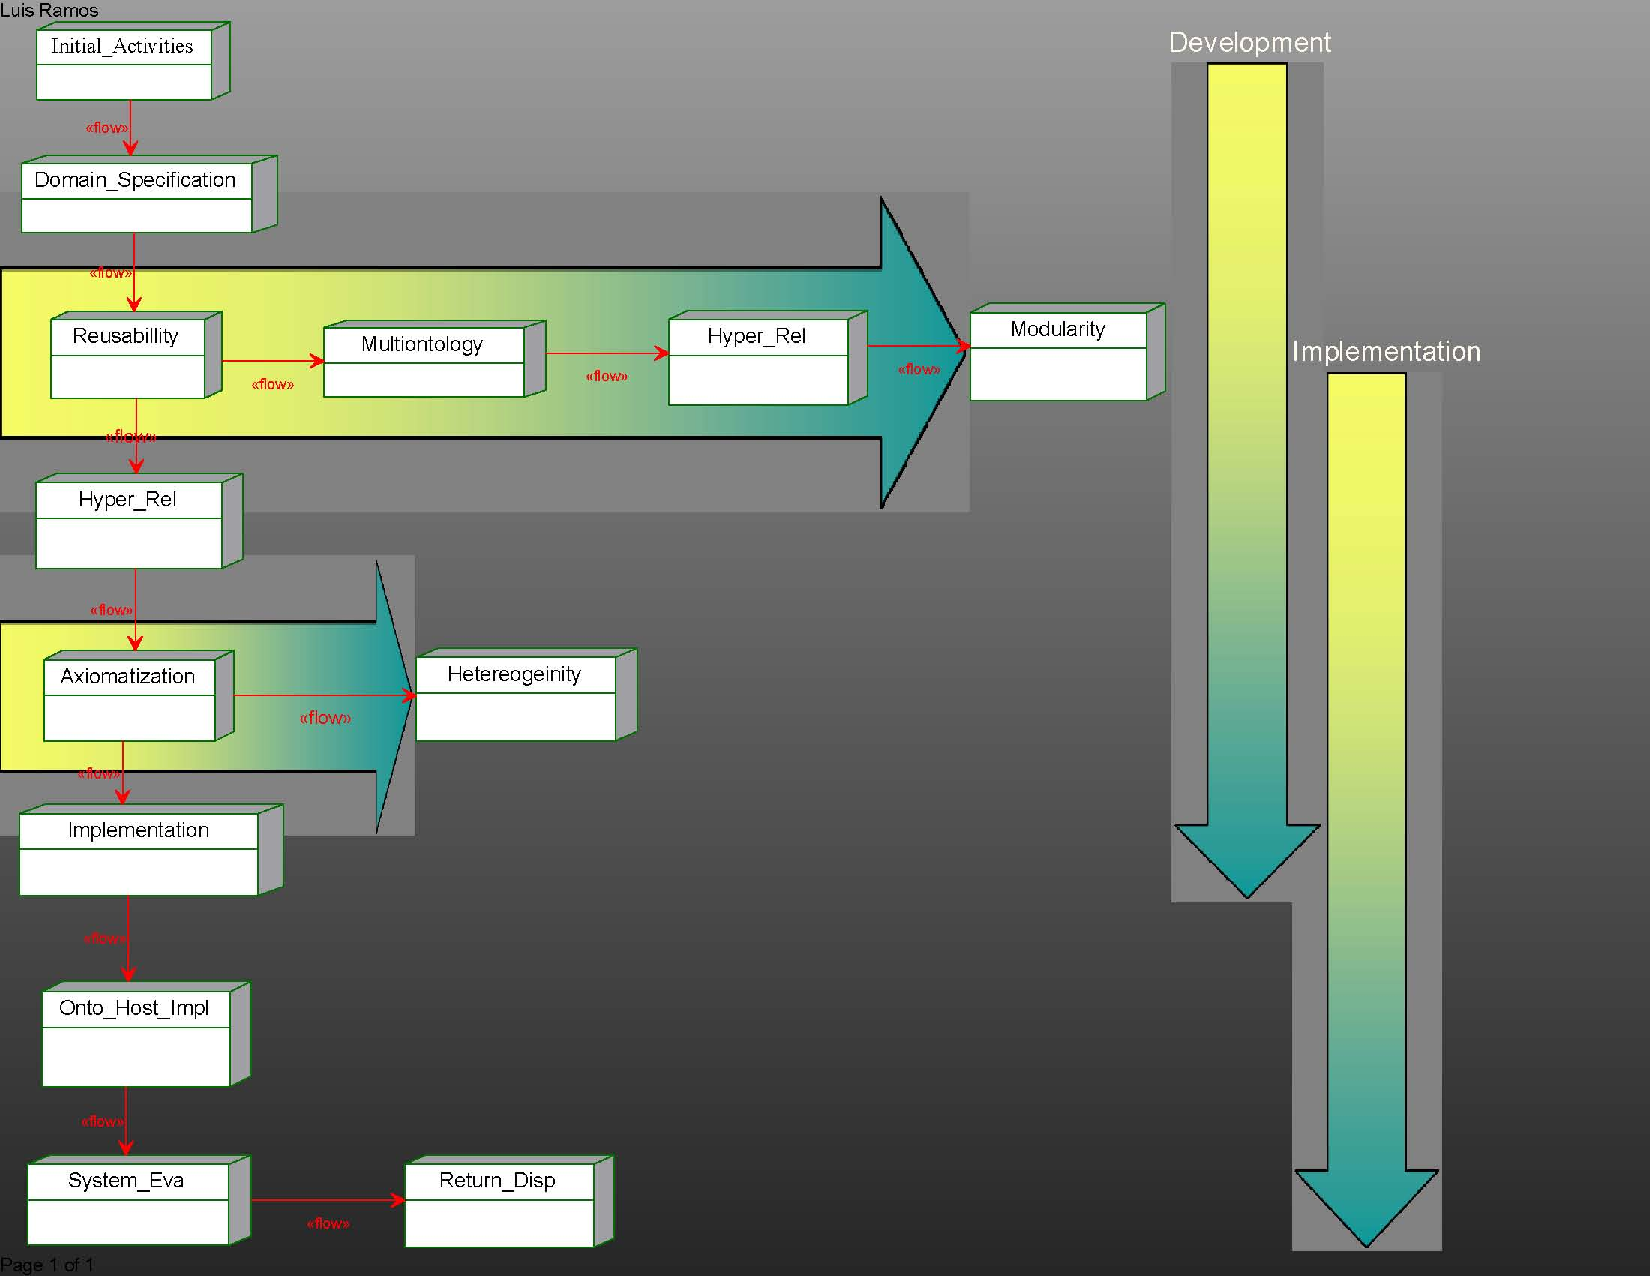
\includegraphics[scale=0.7,angle=90, totalheight = 0.8\textheight, trim=0.3cm 0.3cm 0.3cm 0.3cm, clip=true]{figure-chapterIII/figure3-22}\\
		\caption{My Methodology}
		\label{figure3-1}
	\end{center}
\end{figure}

 
We included the \textbf{Reusability}\footnote{https://github.com/luisenriqueramos1977/OntoSmart/wiki/Reusability}as a subactivity of \textbf{Modularity} because ontologies promised to be artifacts for interoperability. But to achieve this, ontologies should be managed as standardized artifacts (i.e., pieces of software). However, in most cases the use of ontologies is developed from scratch, limiting reusability and interoperability as well. In this vein, we consider worth including activities reuse and an indicator to measure reutilization level. These activities reuse consist on the following subtasks:

\begin{itemize}
	
	\item \textbf{Finding ontologies related to the target domain}\footnote{shorturl.at/gDFKZ}
	
	\item \textbf{Quality  assurance from the information point of view}\footnote{shorturl.at/bimL6}
	
	\item \textbf{First check of ontologies against requirements}\footnote{shorturl.at/dfgxT}
	
\end{itemize}


From the above described scenario we have the following possible outcomes: first, to find a fully reusable ontology is an ideal situation; second, to require development from scratch, third to develop an ontology using parts of others and fourth to reuse modular ontologies. 

To analyze the fourth scenario we require:

\begin{enumerate}
	\item Ontologies related to a common domain as input.
	\item A software tool for mapping and merging ontologies.
\end{enumerate}


Then, the current task consists in mapping all ontology against each other, so we can obtain ontological commitments amongst them.  The resulting mappings per pair of ontologies will be recorded and are maintained as a hyper-ontological structure over modules. 

At this point we should have one of the following options available: 

\begin{itemize}
	
	\item[1]. One ontology, if we have developed one from scratch, 
	\item[2].- One ontology developed from a group of ontologies, or 
	\item[3]. A set of linked (or to be linked) ontologies for reuse.  
	
\end{itemize}

After having a modular structure, we have to evaluate the necessity of \textbf{axiomatization}. That is because from the intended use of ontology, it is possible to draft the axiomatization requirements for our ontology or ontologies. In this case we need to define whether or not we need lightweight or a heavyweight ontology\footnote{https://github.com/luisenriqueramos1977/OntoSmart/wiki/Axiomatization}. As we indicated above, the existence of heavyweight ontologies indicates that the axiomatization process should be carefully considered in order to determine if the target language constructors are expressive enough to reach the expressiveness level required to fulfill our requirements. We have to be aware of the presence of n-ary relations (higher than binary), mereotopological relations, procedural reasoning and different unit systems. The  aforementioned  requirements  could possibly  enhance the expressiveness level of any language using them in a higher level. If any of them are present in the ontology or ontologies, limiting the full implementation of our model, then we should proceed with the \textbf{hetereogenity}\footnote{https://github.com/luisenriqueramos1977/OntoSmart/wiki/Heterogeneity} Building Block to determine if a heterogeneous layer is required. Otherwise, we can proceed with system implementation. In the \textbf{Implementation} Building Block, as most of Ontology methodologies, we should implement the developed ontology. However in this case, given that this methodology is centered in reutilization, it is highly likely that we should just have our ontology or ontologies developed in an ontology language. 









\subsection{Ontology Model and Evaluation Neccesity}\label{3.2.4}

Ontology corresponds to a simplified model of reality, which is additionally proposed to be used as an interoperability artifact; this last requirement means that ontology should be reused within  a given domain or a set of related or overlapping domains. We can then assign a quality attribute to our ontology as we currently do with any other artifact,  offering the final user a reference of the quality of the ontology as a reusable product. 

In science, quality measurement is mostly related to variables of \textit{accuracy} and \textit{precision}.  In regard to ontology quality measurement, there is no general agreement on what has to be measured, whether ontology is a product or a given application based on ontology. According to our criteria, the   lack of agreement of quality measurement occurs because of the categorization of ontology presented in Fig. \ref{figure2-1}. Meaning that some ontologies are not developed to be used directly in applications, limiting their evaluation in an application-centered approach, while others are developed for a given application. Therefore, we divide our evaluation process as follows:


\begin{enumerate}
	
	\item[1].	 Evaluation based on the inputs, product and development process
	This evaluation is self-subdivided into the following stages:
	

	\begin{enumerate}
		
		\item[a.] Input quality assurance, through the input ontology evaluation procedure.
		
		\item[b.] Structure measurement, implementing the metrics recommended   by \cite{manouselis_exploring_2010}. These authors are of the criteria that empirical studies are needed to validate how different metrics are capable of judging deciding about quality properties and their interpretation. They developed a tool called Ontometrics, which considered metrics indicators such as Number of classes (noc), Number of Instances (noi), Number of Properties (nop), Number of Root Classes (norc), Number of leaf Classes (nolc), Averagea Population (ap), among others. 
		
		\item[c.] Modularity  , as a criterion to classify patterns, is mostly to provide judgment about quality.  Considered that implanting wrong patterns will affect the quality of the system as a whole. \cite{randelli_introducing_2010}.
		
		\item[d.] Reusability, as an average metric for reutilization, will indicate how interoperable   the system is by using inherited terms as a reference. For this task we will follow a criteria similar to the proposed by \cite{spiliopoulos_discovery_2010}, with the difference that we considered no pair, but networks of ontologies. 
		
	\end{enumerate}
	
	\item[2]. 	Evaluation related with functionally and implementation
	
	This evaluation is, in our opinion, the most crucial one, but it is subject to the system development. In other words, this evaluation will take place only when some functional part of the system is able to carry out certain tasks. For a successful evaluation, developers should have previously categorized activities, their complexity level, similar to having a list of competency questions to be answered. The criterion to define complexity will be:
	
	
	\begin{enumerate}
		
		\item[a.] If the answer to a query, or to carry out some task can  be done  through ontology, or consultation is required  for other ontologies in order to provide the required answer, or carry out the task.   
		
		\item[b.] If a decidable language is required to  execute  the corresponding tasks, but the chosen languages are not expressive enough to represent the required knowledge in the knowledgebase, such scenario will obligue us to consider a  heterogeneous framework. .  
		
	\end{enumerate}
	
\end{enumerate}


\section{A Semantic Framework}\label{section3.3}

Ontologies were initially introduced as part of the overall system architecture depicted in Fig. \ref{figure2-7}, which means they are not isolated artifacts. In fact, for implementing an ontology based system, it is necessary to deal with related technologies presented in building blocks included in the aforementioned Figure.  Moreover, if there are several interacting ontologies, written with different ontology languages, and logics then it is possible that any ontology shall require a respective architectural structure for being hosted and for interfacing with other ontologies within a Semantic Framework . This Semantic Framework was named by \cite{berners-lee_semantic_2001} as Semantic Web . 

In this subsection we introduce architectures that allows us to deal with ontologies within the Semantic Web, and a general criterion  for using them in applications. 









In this Chapter we proposed a new methodology that integrates two fundamental approaches into the Ontological Engineering, those are modularity and heterogeneity. This methodology initiates with a quality assurance procedure, followed by specific method to decide when modularity and heterogeneity are required. We provides tools to support the workflow along the methodology. Furthermore,  we introduced some required technologies for implementing the proposed methodology. 

In next Chapter, we will present the results of implementing the just described methodology in the domain of manufacturing.
    \chapter{RESULTS}\label{chapter4}

In this Chapter we will go throughout the steps proposed in the methodology depicted in Fig. \ref{figure3-1} of Section \ref{section3.1}. The motivation for this methodology comes from the integration of the ontology methodologies described in Section \ref{subsection2.2.6}, and the heterogeneity approach introduced in Section \ref{figure2-3}. The general steps are domain specification or definition, deciding about modularity, deciding about heterogeneity, implementation and evaluation. We will address each in turn. 



\section{Initial Activities }\label{section4.1}

Manufacturing has been our discussion topic from the Introduction to now. However, given that several types of products can be included under this topic, we consider it necessary to define the scope as accurately as possible. This work  focuses on products that can be represented through a specific geometry. The products to be considered will therefore be goods (mechanical parts), not services, which consist of one, two or three-dimensional parts, and can be modeled with CAD tools, and manufactured with a set of automatic machine tools. This might require the interaction of various machines to obtain the finished product. Moreover, it should be possible to modify the final product in order to fulfill all the customers’ possible demands.

The automation to be discussed will cover the automatic validation of designs based on machine and product features, as well as production restrictions  in order to improve productivity and reduce time to markets \citep{dorr_cad-cam_1987}.No code will be generated to program any specific commercial machine. Instead: the existing upper ontologies which have been developed and that can be useful for the stated objectives will be used following the basic ontology reuse principle. The complete life cycle of the product will also not be covered as well, where  interaction with customers, distribution or logistics of the product and marketing behavior will not be addressed. These issues can be considered for future work where the complete life cycle of the product will be covered.

\subsection{Domain Specifications }\label{4.1.1}

Given that we limited the type of products to mechanical parts, our target designs and features are those related to the machining process. These are: drilling, cutting, punching, and shearing among others. 

We now present some examples of possible scenarios that can arise when dealing with Automated Features Recognition and Design validation, and which constitute the main target of our research.

\begin{itemize}
	
	\item \textbf{Scenario 1}: When a designer creates a new product, it is a common fact that the designer is only focused on the functionality from the user’s point of view. As soon as the product design  is completed, it is sent to the manufacturing engineer who may determine that the product cannot be manufactured due to factory restrictions. Consequently, the designer has to modify the design in order to accommodate the given recommendation. 
	\item \textbf{Scenario 2}: A manufacturing engineer needs to generate a process plan for a new or modified product, based on a digital design of the product itself. Most of the time  engineers use   their own experience and knowledge about the facility, machines and raw materials. For instance, the designer may decide to use a new raw material due to its higher corrosion resistance, but without having the possibility of indicating in the digital design that such raw material has a higher mechanical   resistance. As the manufacturing engineer does not see any change in shape, producing   waste of raw material, because of the lack of information exchange between designer and manufacturer. Furthermore, as we indicated in Section \ref{section2.1}, the workflow described in this scenario is mostly carried out in an automatic or semiautomatic manner, thus human intervention is reduced. Of course, reducing human intervention we increase productivity, although certain type of issues are harder to find by current information systems. Consequently, design mistakes can affect the manufacturing process production can waste raw materials. 
	
	\item \textbf{Scenario 3}: A group of investors is interested in offering a new product because market research has demonstrated that the product is highly innovative, and is likely to be well accepted. These investors also know that the technical resources (raw material and machinery) are going to have a high cost, requiring a detailed cost evaluation to determine its profitability. Furthermore, investors also know that market competition has the same information, and they require to make their decisions on producing it, and if favorable, place the product on the market as soon as possible. Therefore, an economical evaluation of the project is urgently required, and gathering information from several distributed sources becomes indispensable. 
	
	
	
\end{itemize}


In Section \ref{section2.4} we described how some authors integrate ontology and the semantic web into the manufacturing domain. Despite the benefits of the research listed, in Section \ref{subsection2.4.3} we included a group of issues relating to ontology and manufacturing that remain open to date. Then, considering the three scenarios described above, we can declare our ontology specific objectives as follows:


\begin{itemize}
	
	\item To enhance manufacturability evaluation of new products by integrating digital designs with raw materials specifications and manufacturing constraints of the latter.
	
	\item To improve concurrency of factory main components. This improvement is obtained by enabling virtual modeling and providing communication among them. 
	
	\item  To integrate products, processes and resources specification data into a digital production model, so that all data can be accessed and interpreted by existing software systems and tools.
	
\end{itemize}

\subsection{Competency Questions}\label{4.1.2}

As discussed and explained in Section \ref{subsection2.2.6} the task of posing competency questions is common to all ontological methodologies.  Competency questions are considered as a guide that help define the domain more accurately and a way to obtain application objectives. So, we assume that ontology or ontologies should support the ability to find answers to the corresponding questions. Accordingly, for specific ontologies relevant for our identified goal of providing semantic manufacturing support for physical products, our proposed questions can be listed below. We consider it necessary to remark that as this step is common to most ontology development methodologies, we have found many of the listed questions in previous researchs, for instance in the research of \cite{hepp_references_2013} and  \cite{radhakrishnan_design_1996}. Some further questions are integrated below based on the scenarios and objectives set out in Subsection \ref{4.1.1}:

\begin{itemize}
	\item [CQ1]: is my digital design topologically correct?
	\item [CQ2]: what manufacturing features are present in my product (design)?
	\item [CQ3]: what machinery will enable the performance of a given manufacturing operation?
	\item [CQ4]: what type of machinery is available in the target factory?
	\item [CQ5]: Can the features of a product candidate be manufactured in a target factory with the available machinery?
	\item [CQ6]: Is there any process restriction (e.g the occurrence of an activity A2   shall be preceded by an activity A1)?
	\item [CQ7]: Is the required operation available in a given time space?
	\item [CQ8]: In the case that no machinery is available for manufacturing a certain feature:
	\subitem[CQ8.1]: where can it be obtained? 
	\subitem[CQ8.2]: what is the price?
	\subitem[CQ8.3]: which are the corresponding features?
	\subitem[CQ8.4]: Are they expressed in homogeneous units?
	\subitem[CQ8.5]: what is its replacement cost?
	\subitem[CQ8.6]: which is its official currency?  
	\item [CQ9]: Which are the attributes of the raw material?
	\item [CQ10]: Which is the cost of performing certain machining operations? 
	
\end{itemize}

\cbstart In section \ref{subsection4.2.3} we will implement these CQ's into the respective ontology language of every selected ontology. Thus, according to the number of CQ's answered by ontlogy a quality metrics will be proposed. \cbend


\subsection{Knowledge Acquisition}\label{4.1.3}

This stage is also a common task in ontology development. It seeks to obtain the knowledge to be encoded in our ontology. In section \ref{subsection2.2.6} we discussed how this step has been managed in most methodologies, and we proposed a specific method for identifying and dealing with such sources of knowledge according to the classification proposed in Fig. \ref{figure2-11} and Fig. \ref{figure2-12}:


\begin{enumerate}
	\item Sources of manual knowledge extraction
	
	Knowledge was manually extracted from documental sources, such as brochures and datasheets. This type of documents is characterized because of their specificity  and length, mostly short documents of no more than one or two pages with specific information of products. It is necessary to mention that, in the manufacturing domain, expert domain knowledge is required for interpreting and analyzing  documents containing standard specifications.   
	
	Consequently, in this case the implicit knowledge is made explicit through listings, tabling and defining ontological elements (types, individuals, properties, etc.). This knowledge is used to develop an ontology of CAD and sheet metal parts features. 
	
	\item Sources of  automatic knowledge extraction.
	
	Knowledge automatically extracted from digital documents, which we divided into three categories:
	
	\begin{itemize}
		\item Design standard files: Digital designs represented in DXF, IGES and STEP standards were used to automatically extract data and to populate the ontology. A previous manual review of the respective standards was necessary. 
		
		\item Ontology standard files: The ontology   languages mentioned in Section \ref{section2.2}, were RDF, RDFS, OWL, KIF and CASL, considered in the form of a specific ontology directly or indirectly related to the target domain. Thus, this analysis not only considered the encoded knowledge, but also the features of the respective language.
		
		\item General purpose formatting files: These files comprised general  text    files, PDF, XML, HTML, and XHTML among other formats. These types of files mainly corresponded to products, machinery and other product descriptions. Because of their particular unstructured format and quantity, the use of specialized ontology tools was necessary, for example, like the ones listed in Table \ref{table4.1}. There, Gate can be highlighted as a tool for extracting semantic information, and populating ontologies from text.   
		
	\end{itemize}
	
\end{enumerate}


\section{Finding and Measuring Ontology Quality}\label{4.2}

In Subsection \ref{subsection3.2.1} the steps of our methodology were mentioned as a possibility for the reutilization of existing ontologies. In comparison with the large number of ontologies that have been developed in other domains, such as medicine and biology among others, ontologies related directly or indirectly to manufacturing are fewer.  However, modeling products and processes is a current concern for Ontological Engineering, as evidenced in the list of ontologies mentioned in Section \ref{section2.4}. It is worth remarking that according to the description made in that section, the development of ontologies was not limited to only individual ones, but to propose ontology networks such as TOVE and SWOOP. 

In the following subsection our search process is explained in detail. 


\subsection{Finding Ontologies}\label{4.2.1}

Finding Ontologies is a requirement for reusability that can be considered as a part of the “Reusability” activity shown in Fig. \ref{figure3-1} in Chapter \ref{chapter3}. There we made use of the ontology search engines mentioned in Subsection \ref{subsection3.2.1}. The keywords used were the ones proposed by \cite{martin_design_2003} and \cite{lastra_ontologies_2009}, who have discussed that the terms \textit{product}, \textit{process},  \textit{resource} and \textit{equipment} are considered as higher level concepts in the manufacturing domain. Every ontology reference we found through this tool was recorded, and the list of ontologies finally tabulated.

Table \ref{table4.1} lists ontologies found by this procedure explained above. Results are presented by publication year. The corresponding domain or concept covered by each ontology is indicated in the second column. Some ontologies were developed with a large scope, and due intended to cover many domains, therefore more than one domain is listed in the respective column. Another aspect worth mentioning is that most of the ontologies shown were implemented in OWL: more precisely 70\%, while only 30\% were implemented in FOL. But, from the FOL ontologies, 50\% were published over 15 years ago. In fact, before the publication of the first OWL version, ontologies were written in FOL and KIF. Since then OWL became the preferred ontology language. 

At the bottom of the table several ontologies are highlighted because they were published during the production period of this research. It becomes evident that the process of considering ontologies has not been static but dynamic with continuous updates. 

This list of ontologies requires a certain level of quality assurance in order to determine its reusability; in the following subsection this procedure is carried out and results are presented.


\begin{table}[tp]%
	
	\caption{Ontologies Potentially Relevant to Manufacturing.}
	\scriptsize
	\label{table4.1}\centering %
	\begin{tabular}{lccc}
		\toprule %
		Ontology Name \\ (Acronym)	& Domain  Subdomain	& Language	& Year \\\toprule
		
		EngMath	& Resource	& KIF	& 1993 \\
		
		Resource Ontology \\ (TOVE)&	Resource &	FOL	& 1994 \\
		Organization Ontology \\ (TOVE)	& Resource&	FOL &	1998 \\
		Port Ontology &	Resources&	OWL&	2003 \\
		PSL&	Process &	FOL&	2004 \\
		unspcsOWL&	Products&	OWL&	2004 \\
		SWEET Units&	Resource&	OWL	&2004 \\
		MASON&	Resources, Product&	OWL	&2006 \\
		ADACOR&	Resources, Product&	FOL	&2006 \\
		MSE	&Resources, Product	&OWL	&2007 \\
		Beyond STEP \\ Ontology &	Product&	OWL	&2007 \\
		GoodRelations &	Product	&OWL&	2008 \\
		SWOP Product  \\ Ontology&	Product&	OWL&	2008 \\
		Features-Based Design \\ Ontology&	Product	&OWL&	2008 \\
		DFM e-Design &	Product	&OWL&	2009 \\
		Cutting Process \\ Ontology&	Product, Process&	FOL &	2009 \\
		MTM	&Resources&	OWL	&2009 \\
		\textbf{ONTOMoPS}&	\textbf{Product, Process}&	\textbf{OWL}&	\textbf{2011} \\
		\textbf{PRONTO}	&\textbf{Product}&	\textbf{OWL}&	\textbf{2011} \\
		\textbf{OntoSTEP}&	\textbf{Product}	&\textbf{OWL}&	\textbf{2012} \\
		
	\end{tabular}
	
\end{table}


\subsection{First Quality Control}\label{subsection4.2.2}

\begin{figure}
	\begin{center}
		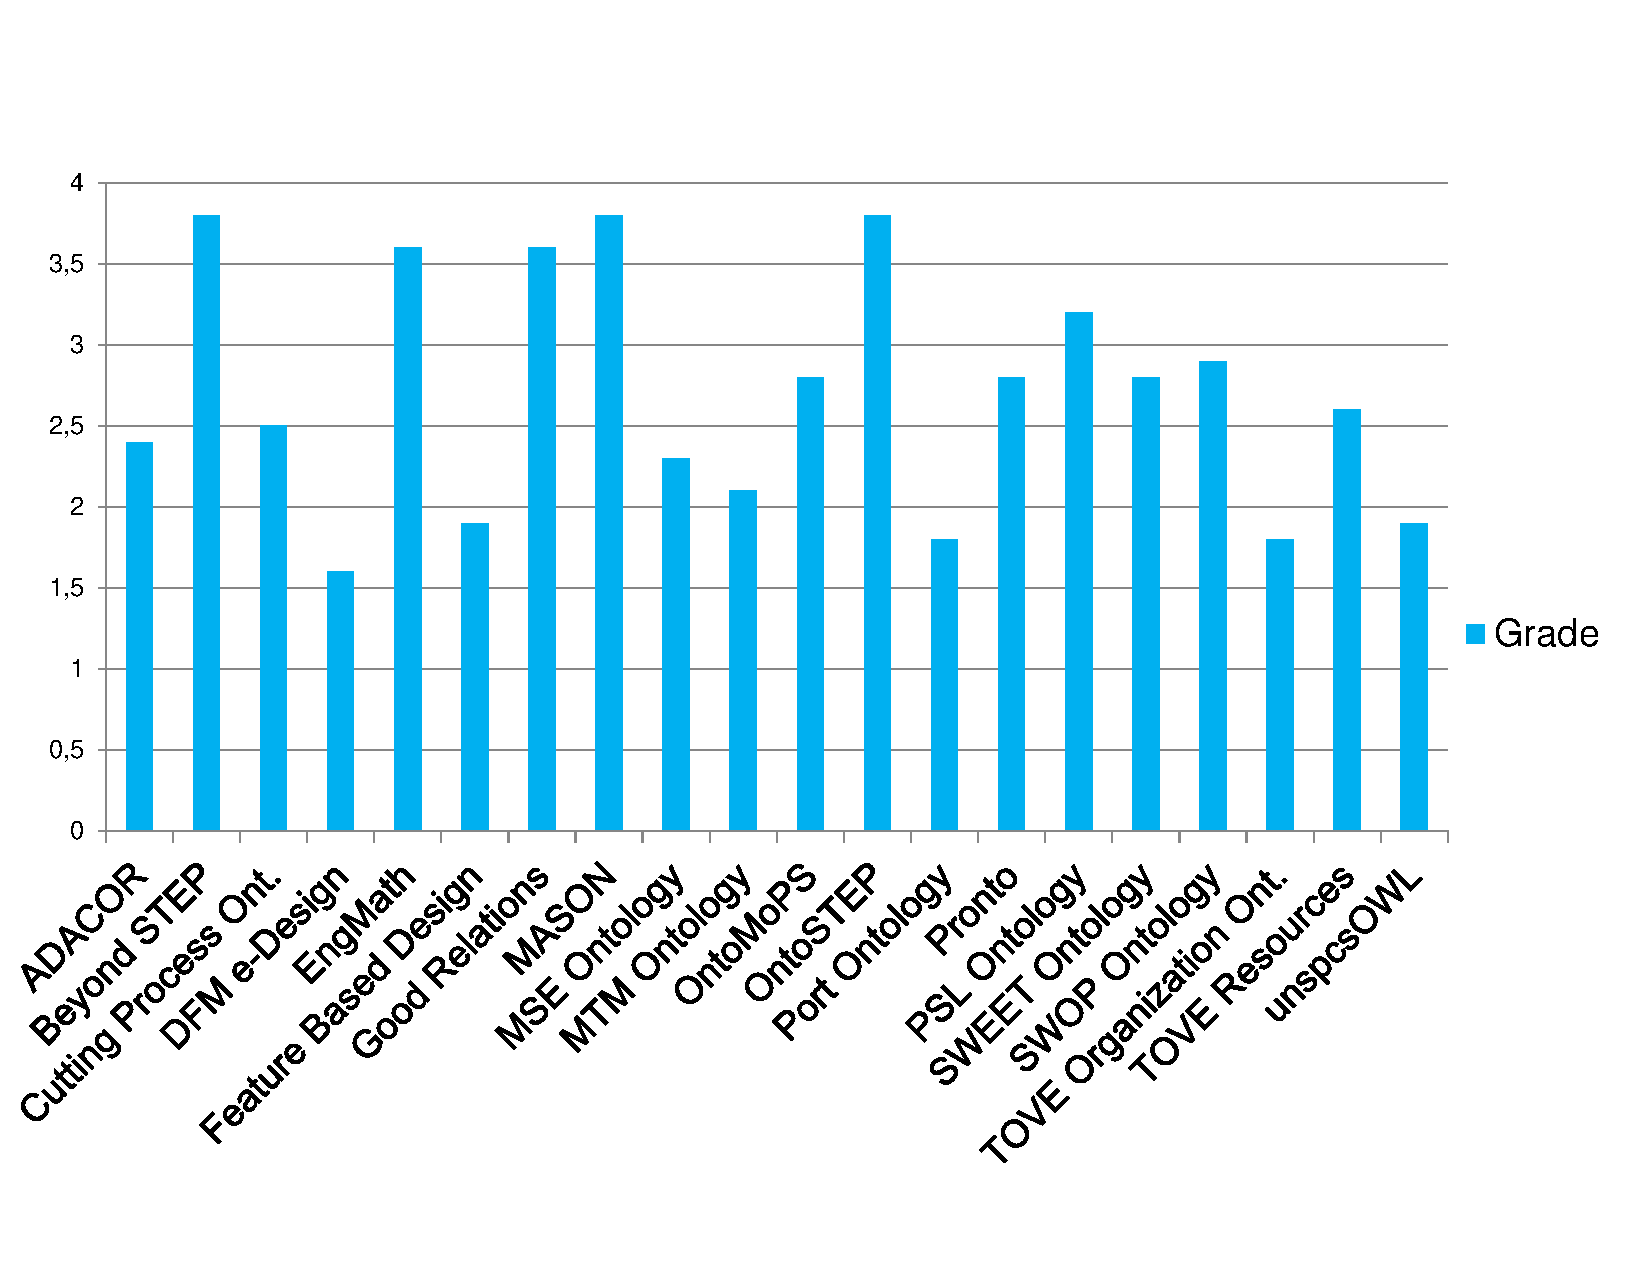
\includegraphics[scale=0.5]{figure-chapterIV/fig4-1.pdf}\\
		\caption{Results of Input Evaluation}
		\label{figure4-1}
	\end{center}
\end{figure}

\cbstart The ontologies listed in Table \ref{table4.1} were submitted to a particular quality assurance procedure as indicated in Subsection \ref{subsection3.2.1}. In that section we proposed to base this quality evaluation on the dimensiones: \textbf{verifiable}, \textbf{integrity},  \textbf{timeliness} and \textbf{reproducibility}. In order to quantify those parameters we built and proposed the questionnaire   shown in Appendix \ref{appendixd}. There, every dimension is presented with a list of weighted scenarios. The value of the scenario is ranging from 1 on an ideal situation to a lower value given to worse or less advantageous scenarios. For instance, in the case of the \textbf{Timeliness} dimension, we considered three possible timespaces for the publication of the ontology: less than two years ago, more than two years ago, but less than five years ago and more than fives years ago. Ontologies published less than two years ago received the highest degree, that is 1; while ontologies published more than five years ago received the worst degree, that is 0.5. The results permitted us determine the current quality level of each ontology. Fig. \ref{figure4-1} outlines the output of performing this preliminary evaluation. \cbend 

According to the results shown here, Ontologies evaluated can be divided into three categories: those with a quality range [4, 3] were considered of high quality and passed to the next evaluation procedure. Ontologies with a quality range (3, 2] were considered of good quality and passed to the next stage. The ontologies within the range (2,0) were discarded.   






A simplified view of these quality sets mentioned above is outlined in Fig. \ref{figure4-2}. From this figure, it can be considered that a reduced number of ontologies fulfill the reusability criterion we proposed in the questionnaire.  That is 30\% appears as highly reusable, while a larger set can be reused   after certain intervention of the ontologists. A last set is of low quality and should not be reused. 


\begin{figure}
	\begin{center}
		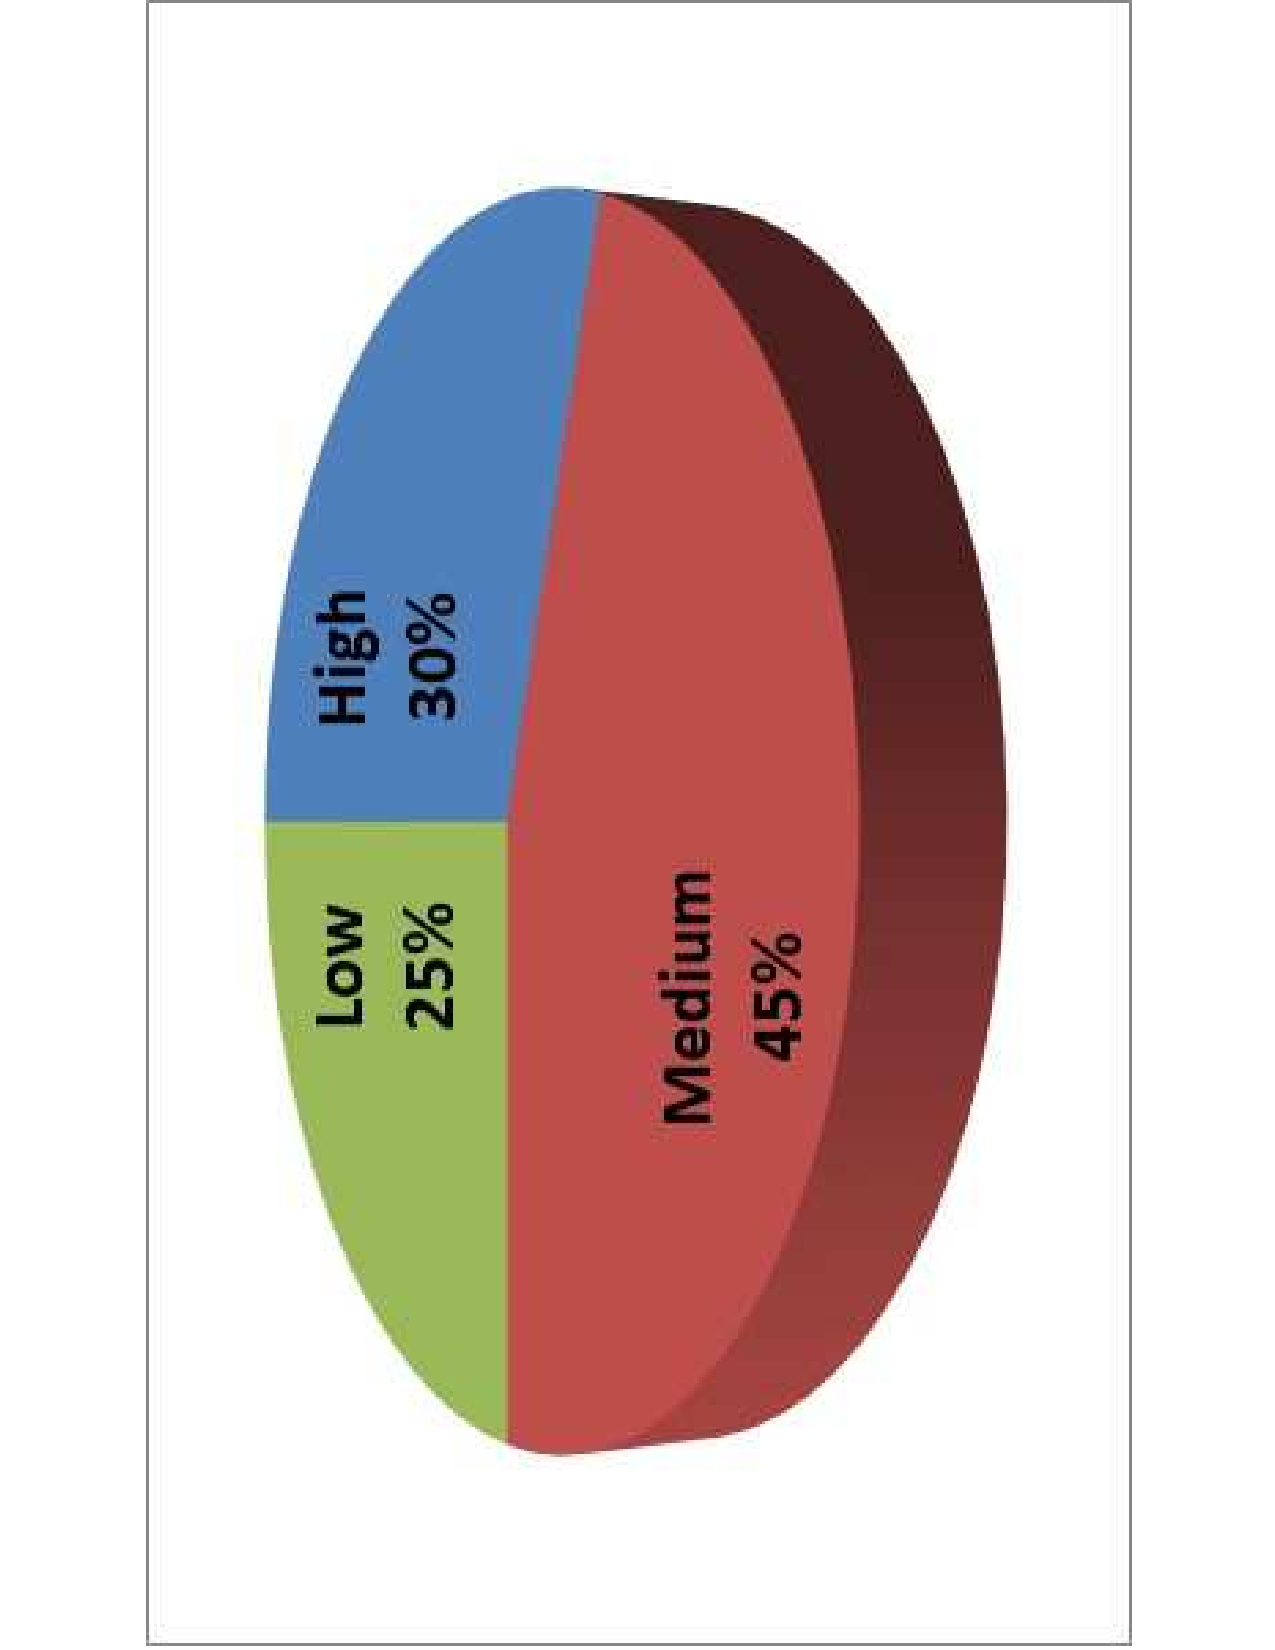
\includegraphics[scale=0.4, angle=-90]{figure-chapterIV/fig4-2.pdf}\\
		\caption{Grouping of Ontologies by Quality Level}
		\label{figure4-2}
	\end{center}
\end{figure}



Reasons leading to a larger set of low and medium quality ontologies are displayed in Fig. \ref{figure4-3} and Fig. \ref{figure4-4}. Firstly, conceptually speaking, ontologies should be publicly available, and with minimum limitations for their use.  However, as Fig. \ref{figure4-3} shows, from our sample ontologies, only 55\% were available for direct download or provided by authors, while the other portion was not. This issue limits the use of an ontology and also reduces the possibility of performing a more accurate evaluation. 


\begin{figure}
	\begin{center}
		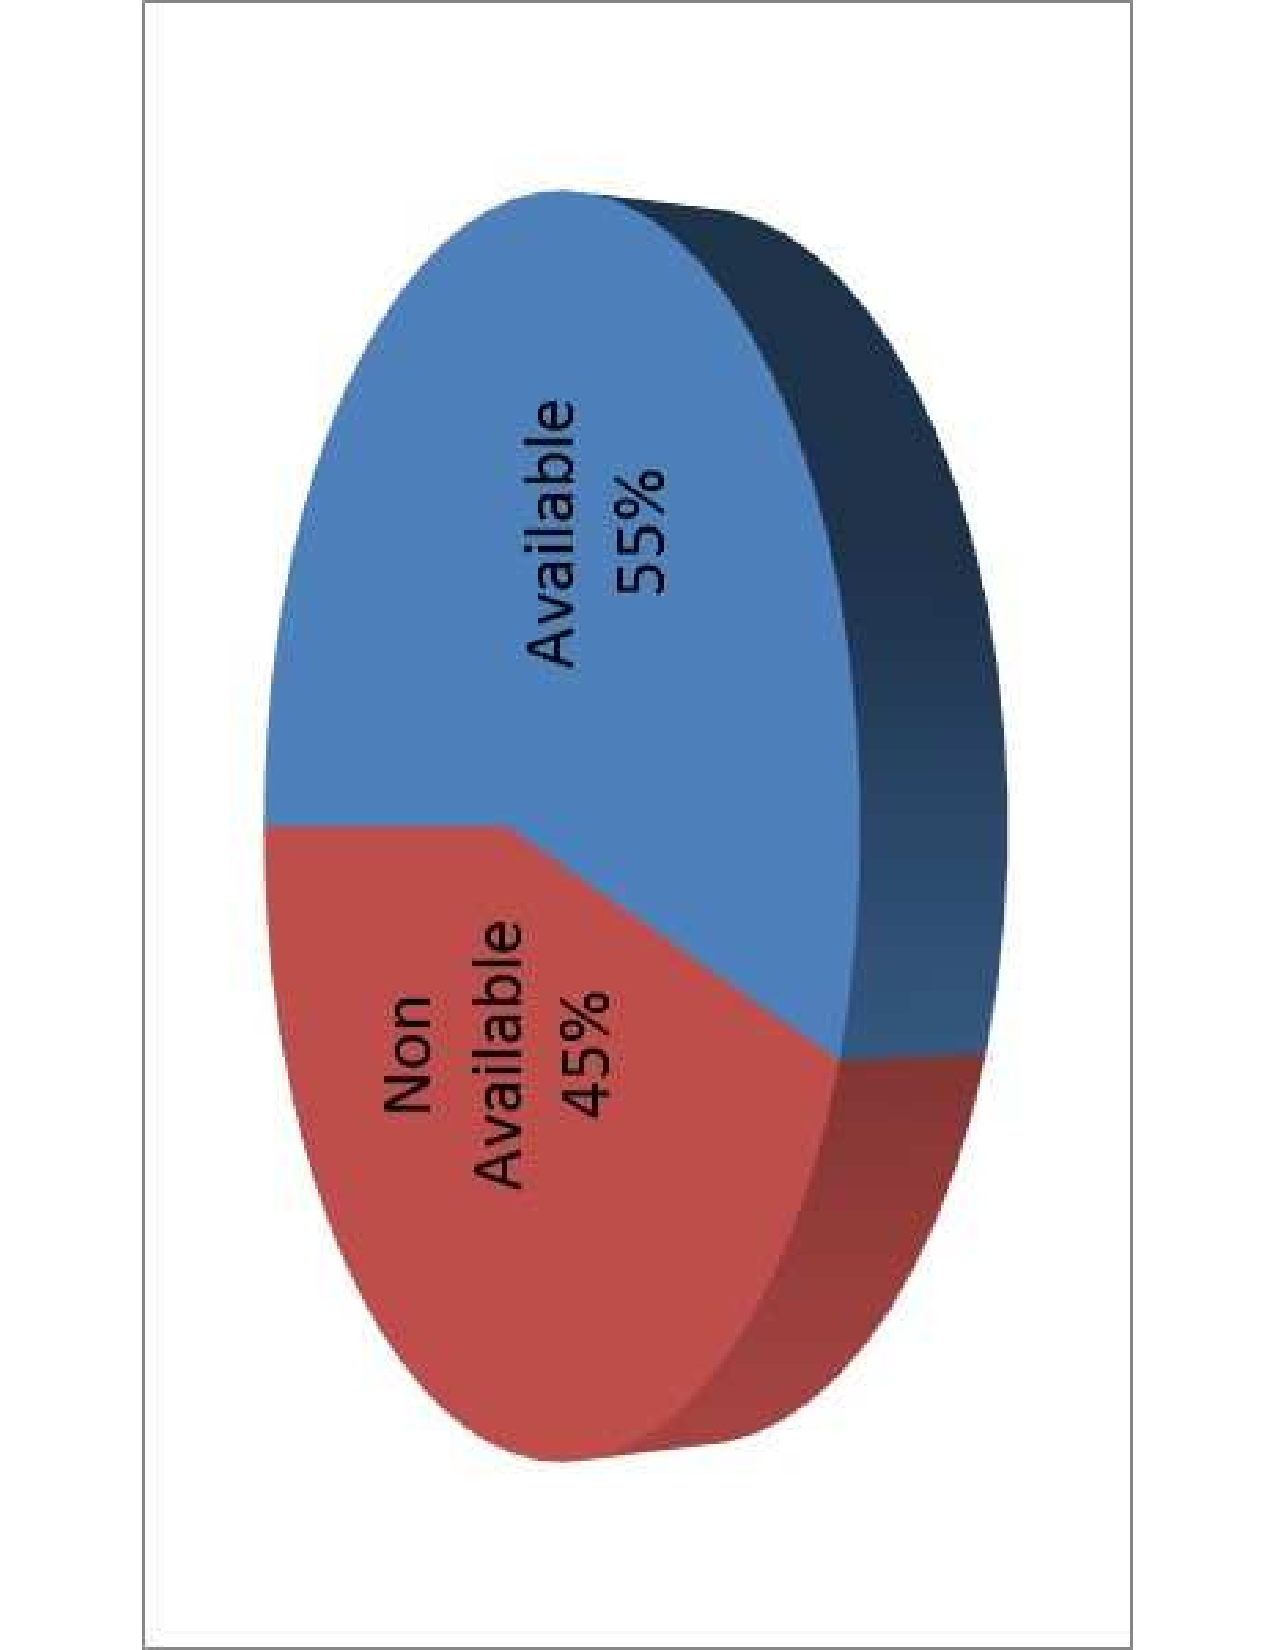
\includegraphics[scale=0.4, angle=-90]{figure-chapterIV/fig4-3.pdf}\\
		\caption{Ontology Availability Evaluation}
		\label{figure4-3}
	\end{center}
\end{figure}



Furthermore, as the next figure shows, explicit indication of rights to reuse and modify the ontology had also been omitted in most of the reviewed ontologies. In an ideal situation, this legal statement should be encoded within the ontology itself, and in the worst case, it should be specified on the site where an ontology is available for download. OWL has a mechanism that makes it possible to add such types of annotations to ontologies, but even in many of the ontologies written in OWL this possibility was not used.

Finishing this first evaluation procedure, ontologies were reordered according to the quality level previously given. Table \ref{table4.2} lists the order in which ontologies will be considered for subsequent uses and evaluation. 



\begin{figure}
	\begin{center}
		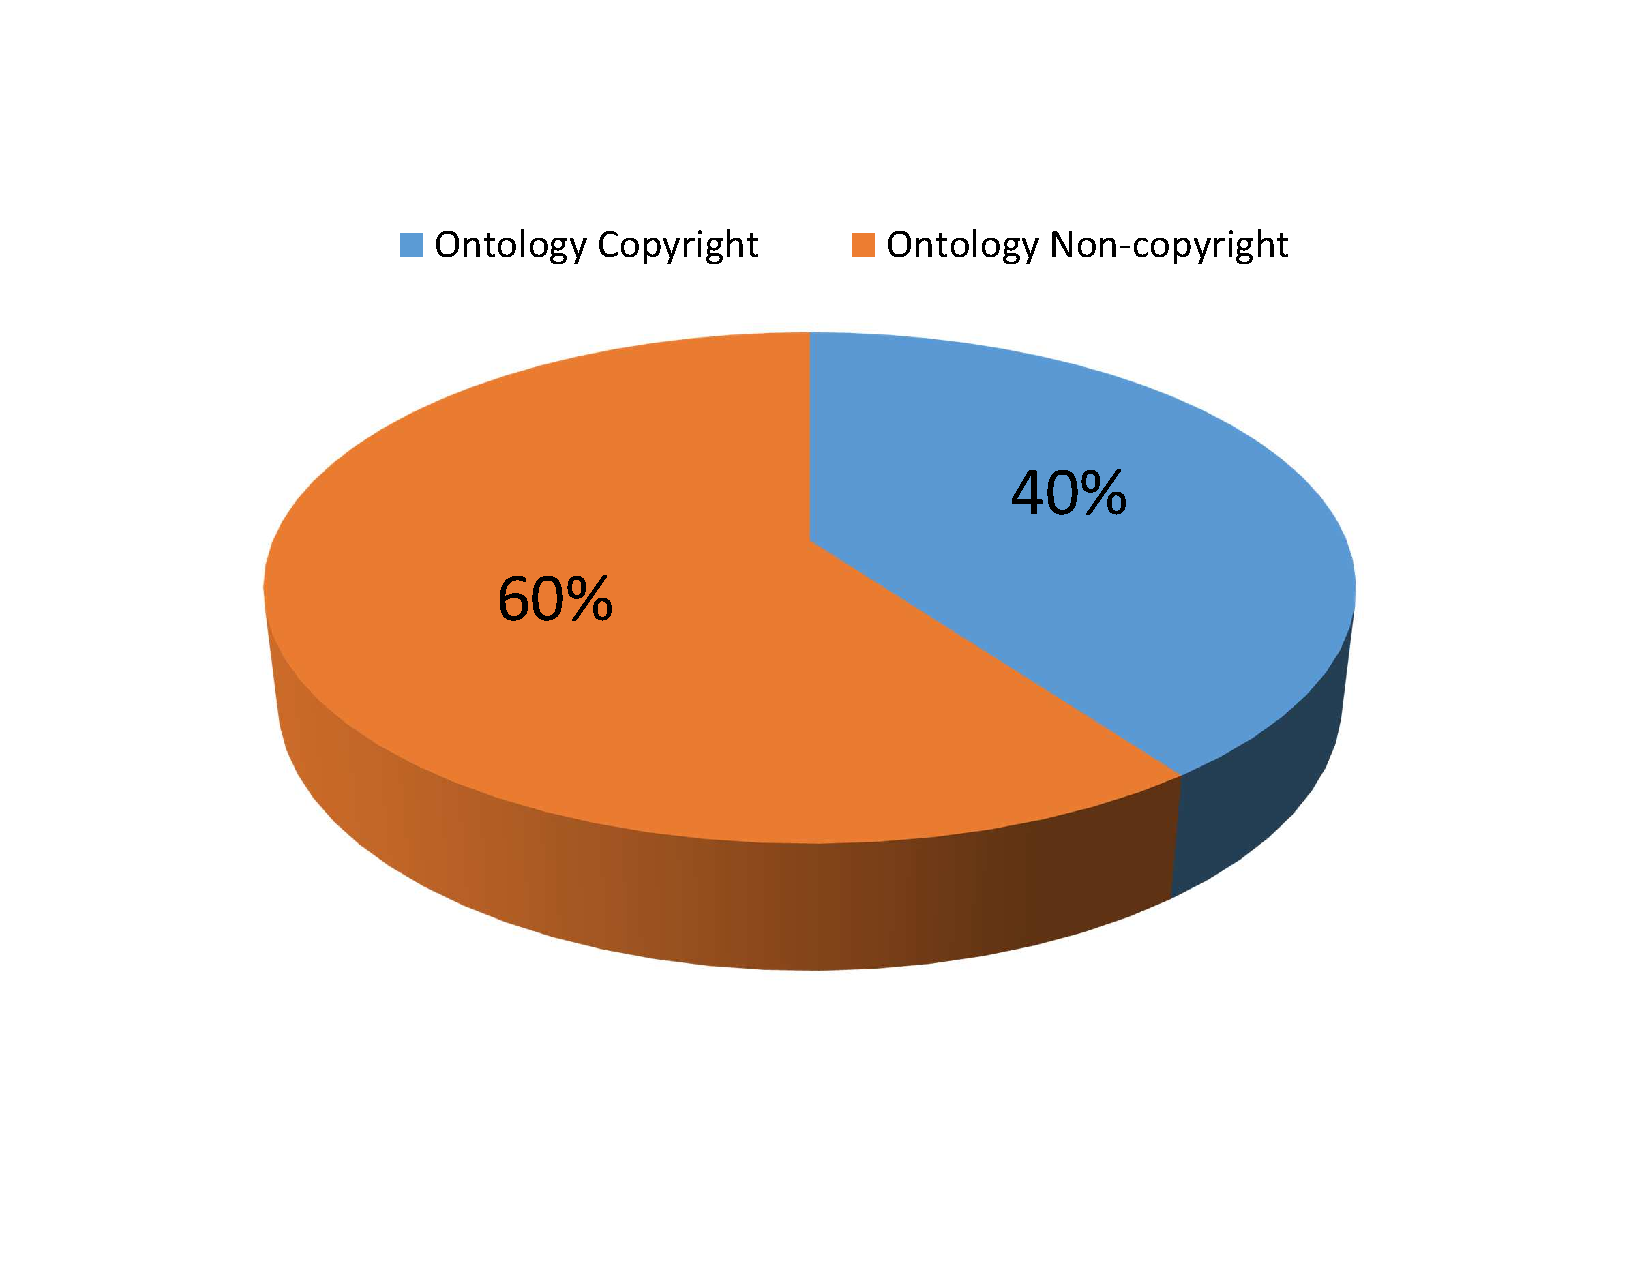
\includegraphics[scale=0.4]{figure-chapterIV/fig4-4}\\
		\vspace{-20}
		\caption{Ontology Intellectual Property Evaluation}
		\label{figure4-4}
	\end{center}
\end{figure}






\begin{table}[tp]%
	
	\caption{Quality Order}
	\label{table4.2}\centering %
	\begin{tabular}{cl}
		\toprule %
		Quality Order &	Ontology Name (Acronym) \\\toprule
		
		\textbf{1}&	\textbf{MASON} \\\toprule
		\textbf{1}&	\textbf{Beyond STEP Ontology}\\\toprule
		\textbf{1}&	\textbf{OntoSTEP}\\\toprule
		\textbf{2}&	\textbf{GoodRelations}\\\toprule
		\textbf{2}&	\textbf{EngMath}\\\toprule
		\textbf{3}&	\textbf{PSL Ontology}\\\toprule
		4&	SWOP Product Ontology \\\toprule
		5&	SWEET Units\\\toprule
		5&	PRONTO\\\toprule
		5&	ONTOMoPS\\\toprule
		6&	Resource Ontology (TOVE)\\\toprule
		7&	Cutting Process Ontology\\\toprule
		8&	ADACOR\\\toprule
		9&	MSE\\\toprule
		10&	MTM Ontology\\\toprule
		
		
		
		
	\end{tabular}
	
	
\end{table}



\subsection{Performing Competency Questions}\label{subsection4.2.3}

The use of Competency Questions to define the scope of ontologies, and additionally to validate them, was explained in Chapter \ref{chapter2}. In Chapter \ref{chapter3} this technique was included as a part of the proposed methodology.   Therefore, in Subsection \ref{subsection4.2.2} a set of competency questions for the manufacturing domain was proposed. Here we mention that if one of the ontologies listed in  Table \ref{table4.2} provides appropriate answers to all Competency Questions, then we can proceed to hosting and implementing that ontology as given in our proposed methodology presented in Section \ref{section3.1}. However, if no ontology fulfills this requirement, then this will require developing a newer ontology, although preferably reusing existing content.  

Competency Questions were performed on the OWL ontologies listed in Table \ref{table4.2} considering their quality order, specifically ontologies  with a quality order in the range from 1 to 3. The Query Tab plugin of the ontology editor Protégé was chosen from Table \ref{table2.1} presented in Chapter \ref{chapter2}. This choice was made because, first both the editor and the Plug-In support OWL, and second because they offer a friendly interface that makes interaction with the chosen ontology possible.  To illustrate this example we chose CQ3 (Section 4.1.2), which in natural language is expressed as follows: which machinery enables the realization performance of a given manufacturing operation? It is worth  mentioning that this query is concatenated with CQ2, which asks questions on product features. Furthermore, CQ3 can be considered as part of the context of scenarios 1 and 3 described in Section \ref{4.1.1}.  In Equation \ref{eq4.1}, this query is formalized with SQWRL.

\begin{equation}\label{eq4.1}
	
	$Machine\_Resource(?m) \wedge enablesRealizationOf(?m,``punching") \longrightarrow sqwrl:select(?m,``punching")$
	
\end{equation}


\cbstart Fig. \ref{figure4-5} illustrates interaction with the ontology. That is, starting with the first ontology presented in Table \ref{table4.2}, that is the MASON ontology, our chosen ontology was manually populated with data. That means, several instances of the concept \texttt{mason:Machine\_resource} were created, and properties of machines were encoded in the ontology, using information of commercial brochures. In this example, a \texttt{mason:Machine\_resource} was related to a  \texttt{mason:Punching} operation by  a \texttt{mason:enablesRealizationOf} predicate. The Query Tab presented in Fig. \ref{figure4-5} is organized according to Protégé vocabulary, therefore from left to right we can view the terms “Class” which is a concept (\texttt{mason:Machine\_resource}), the term “slot” corresponds to a predicate or property (\texttt{mason:enablesRealizationOf}), and the condition “contains”. Within “contains” we will evaluate wheter or not a concept contains a given individual. The resulting individual has to satisfy the condition drawn by the query. In this case the query evaluates whether or not the given instance is “contained” by any individual in the target class by means of a property. In the illustrated case it was possible to find an instance that fullfils our requirement, that is the individual \texttt{mason:Punching\_press}. The result is shown on the right of the figure in “Search Result”. In natural language we can say that we found machinery that enables performance of punching operations, which is a Punching Press. In other words, we found a result for our query. This procedure was followed with every ontology of Table \ref{table4.2}\cbend 


\begin{figure}
	\begin{center}
		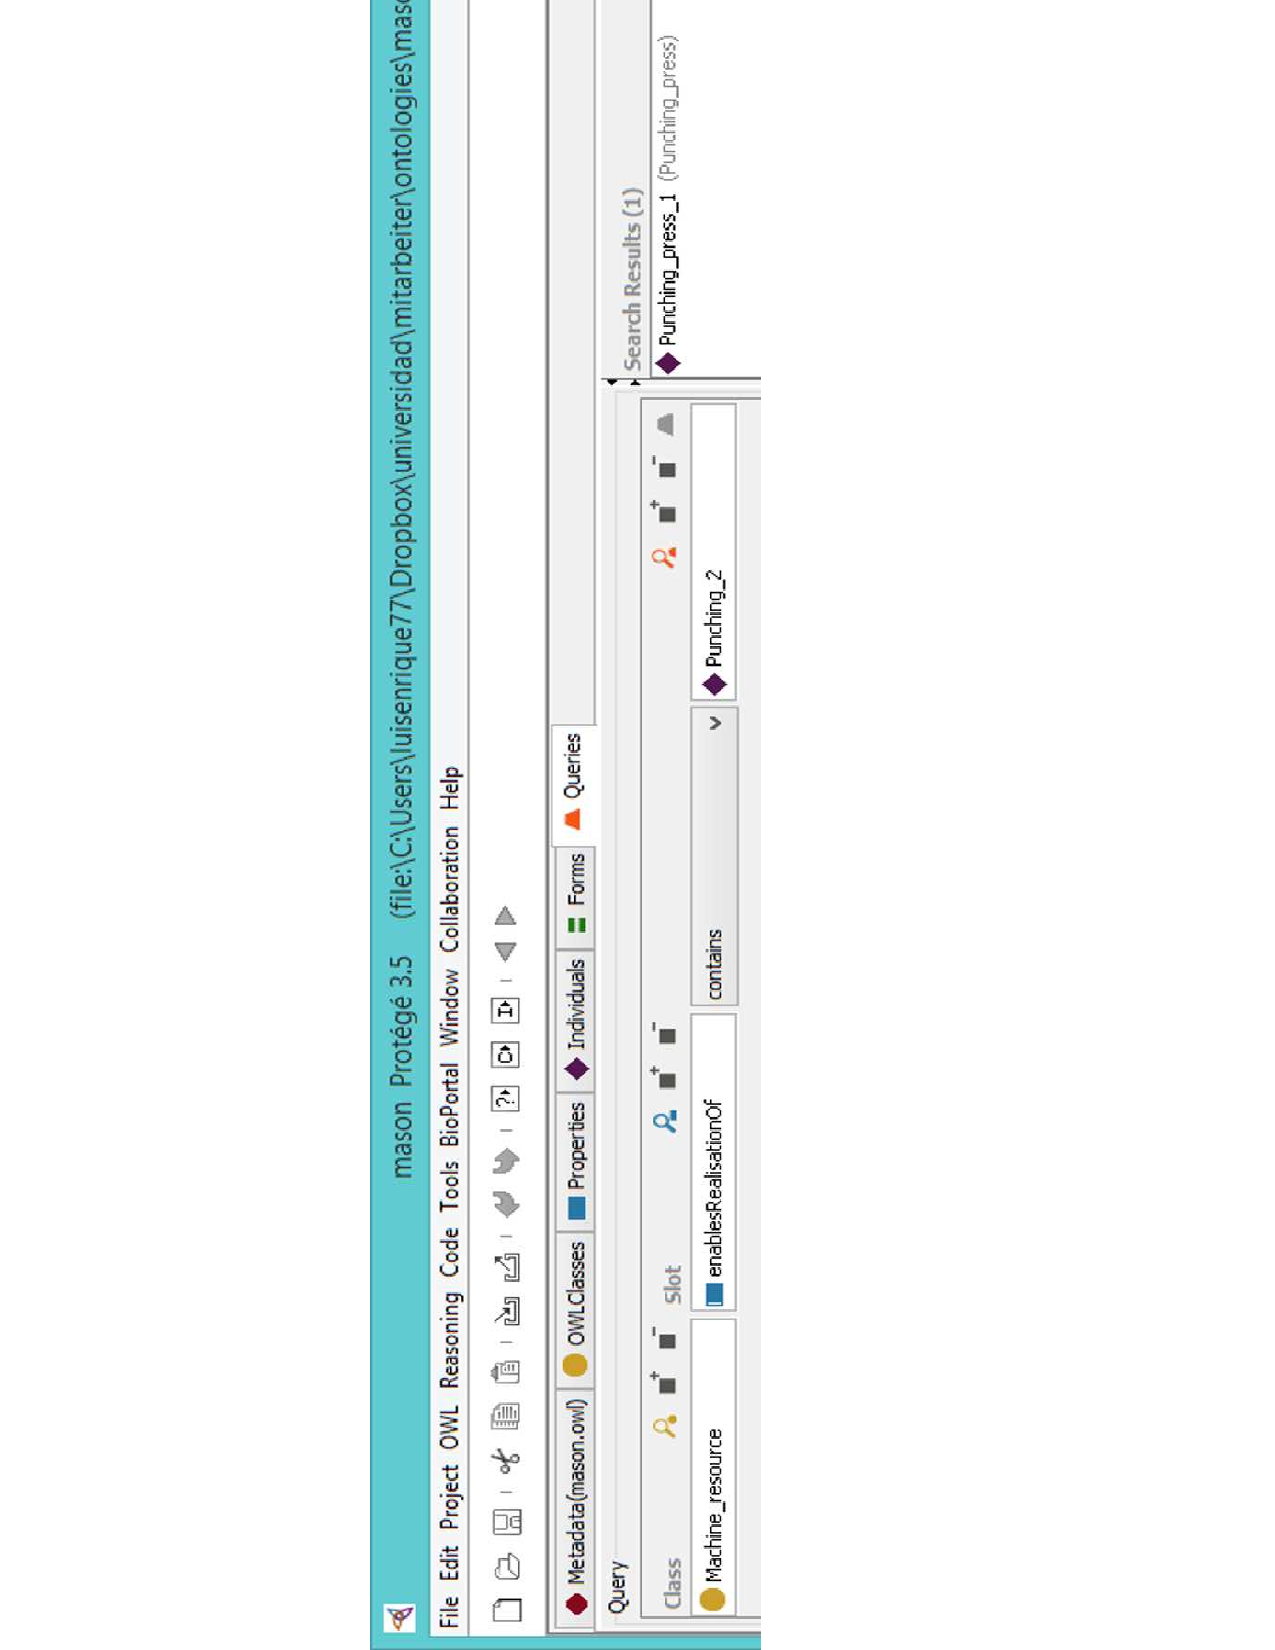
\includegraphics[scale=0.8]{figure-chapterIV/fig4-5}\\
		\caption{Ontology Query in Protégé}
		\label{figure4-5}
	\end{center}
\end{figure}


\begin{equation}\label{eq4.2}
	$
	(defrelation is-occurring-at (?punching ?p) :=
	(and (activity-occurrence ?punching)
	(betweenEq (beginof ?punching) ?p (endof ?punching))))
	$
\end{equation}\\

For ontologies written in other languages (FOL, KIF), questions were considered as answerable when the available terminology (concepts and predicates) could be structured to represent the requirement expressed in the query. \cbstart For instance,   within CQ7 it is required to answer wheter or not an operation or activity is occuring in a given time space. This can represented in PSL as indicated in Equation \ref{eq4.2}. In PLS vocabulary an \textbf{activity-occurrence} or mnufacturing operation \textbf{is-occurring-at} a timepoint \textbf{p} if and only if \textbf{p} is \textbf{betweenEq} the activity occurrence’s begin and end points.PSL therefore supports the required representation of CQ7, and within it we can confirm if a given activity is taking place.\cbend 




Fig. \ref{figure4-6} shows how many competency   questions were answered by each ontology, according to the procedure described above. 



\begin{figure}
	\begin{center}
		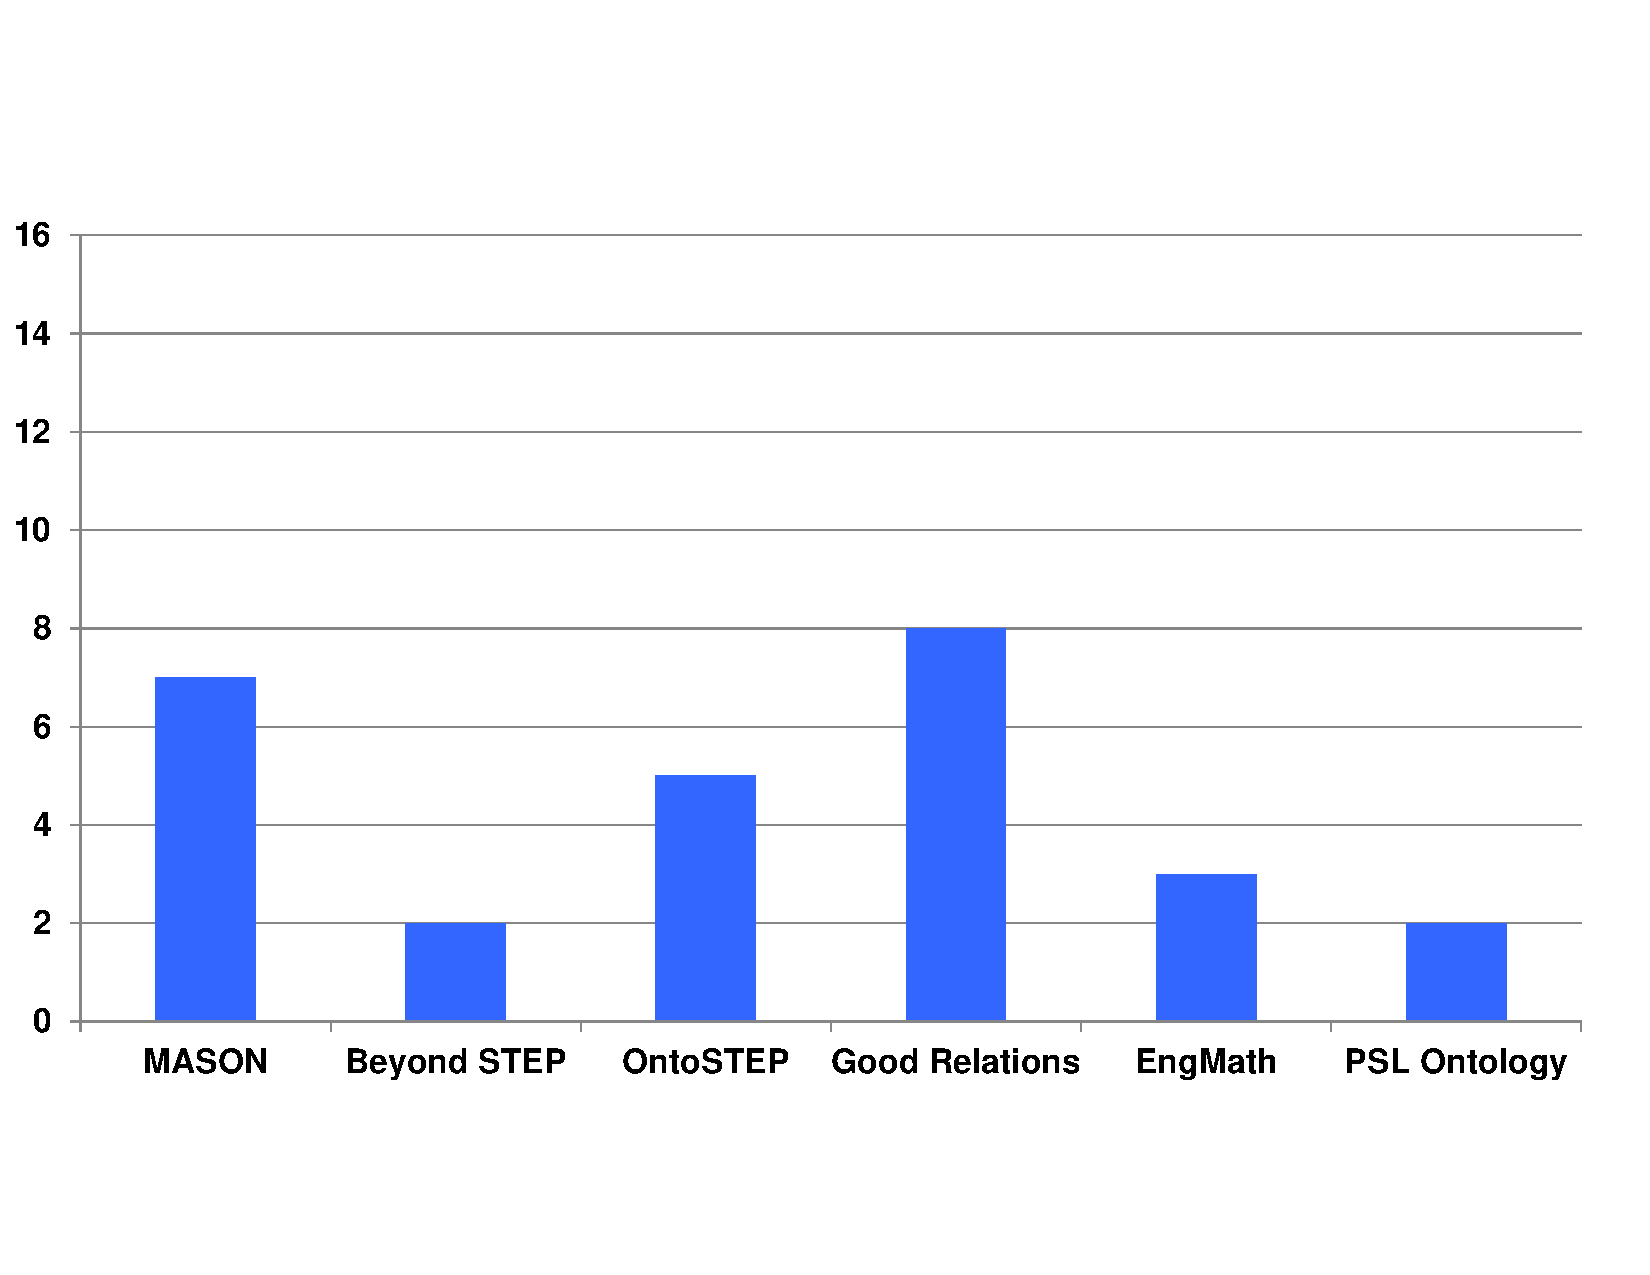
\includegraphics[scale=0.5]{figure-chapterIV/fig4-6.pdf}\\
		\caption{Queries Answered per Ontology}
		\label{figure4-6}
	\end{center}
\end{figure}



If we want to use the number of competency questions answered per ontology as a quality parameter, it could be considered that the quality of selected ontologies is low because most of them represent a quantity of knowledge only sufficient to answer less than 50\% of the questions. Nevertheless, within Fig. \ref{figure4-7} a distributed view can be presented. This graphic breaks down how the selected ontologies \textit{as a whole} provide answers to 15 of 16 queries. Every column represents the number of ontologies that provide adequate answers to the corresponding CQ. For instance, no ontology provides an answer to CQ-3, while CQ-2, CQ-6 and CQ-9 found answers from three different ontologies respectively. 


\begin{figure}
	\begin{center}
		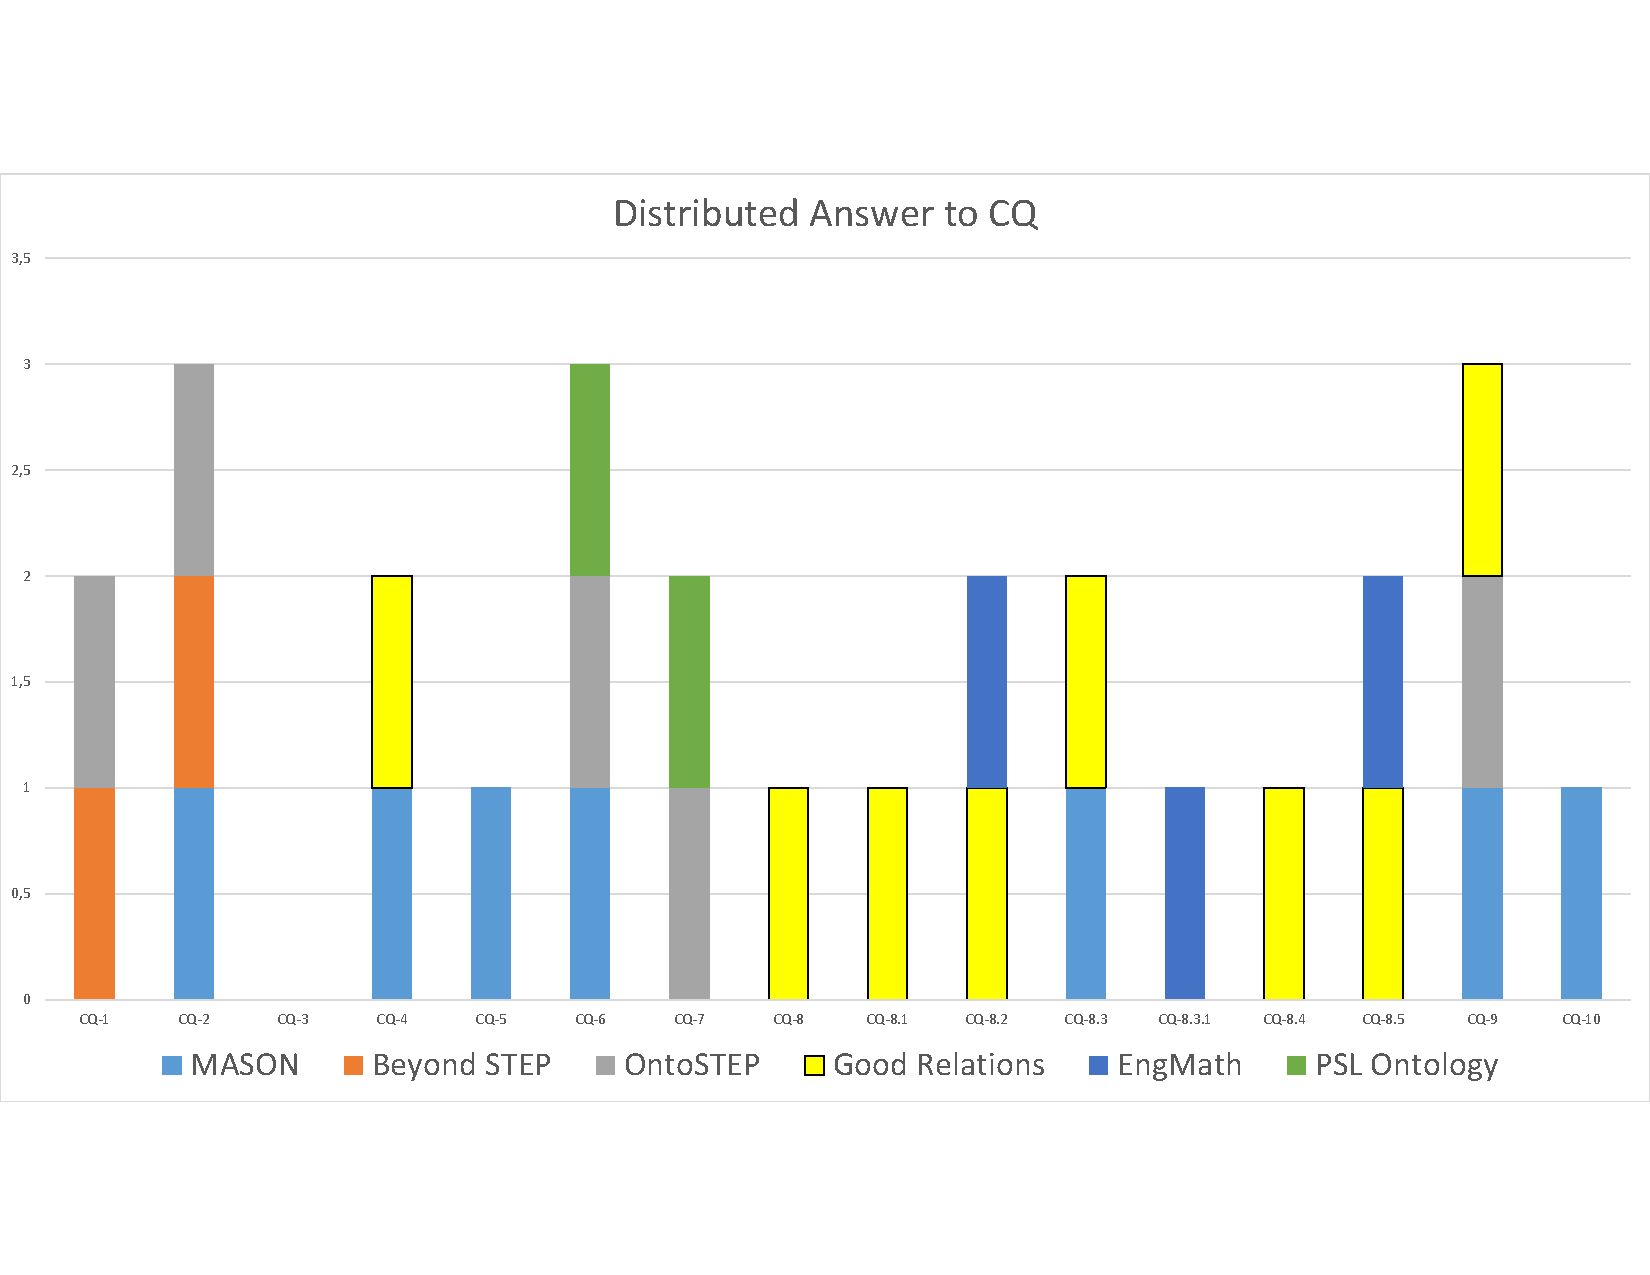
\includegraphics[scale=0.5]{figure-chapterIV/fig4-7}\\
		\caption{Answers Distribution between Ontologies}
		\label{figure4-7}
	\end{center}
\end{figure}



\cbstart From our point of view, answers to these CQ certainly support using \textit{modularity}. That means working with a network of ontologies we can be more efficient in the sense of getting more answer to our CQ's than working with individual ontologies. In other words, while there is no ontology that provides answers for every CQ, many CQ can obtain answers from different ontologies. That means working with these ontologies in a modular architecture, we can obtain answers to 94\% of the given queries, while just using such ontologies alone we would be able to provide answers to only 50\% of the CQ. \cbend 

In fact, more than obtaining an answer for most queries, several ontologies provide an answer to related sets of queries, while many others can be divided into those where the ontology provides an answer to only one query, and others that do not provide answers to any other query.  Such an outcome indicates that, on  the one hand, there is some common knowledge between these ontologies, and it would be possible for a question to obtain answers from different ontologies. On the other hand, there are some questions that obtain answers only from one ontology, indicating that there is certain localized and isolated knowledge in some of them as well. 


\begin{figure}
	\begin{center}
		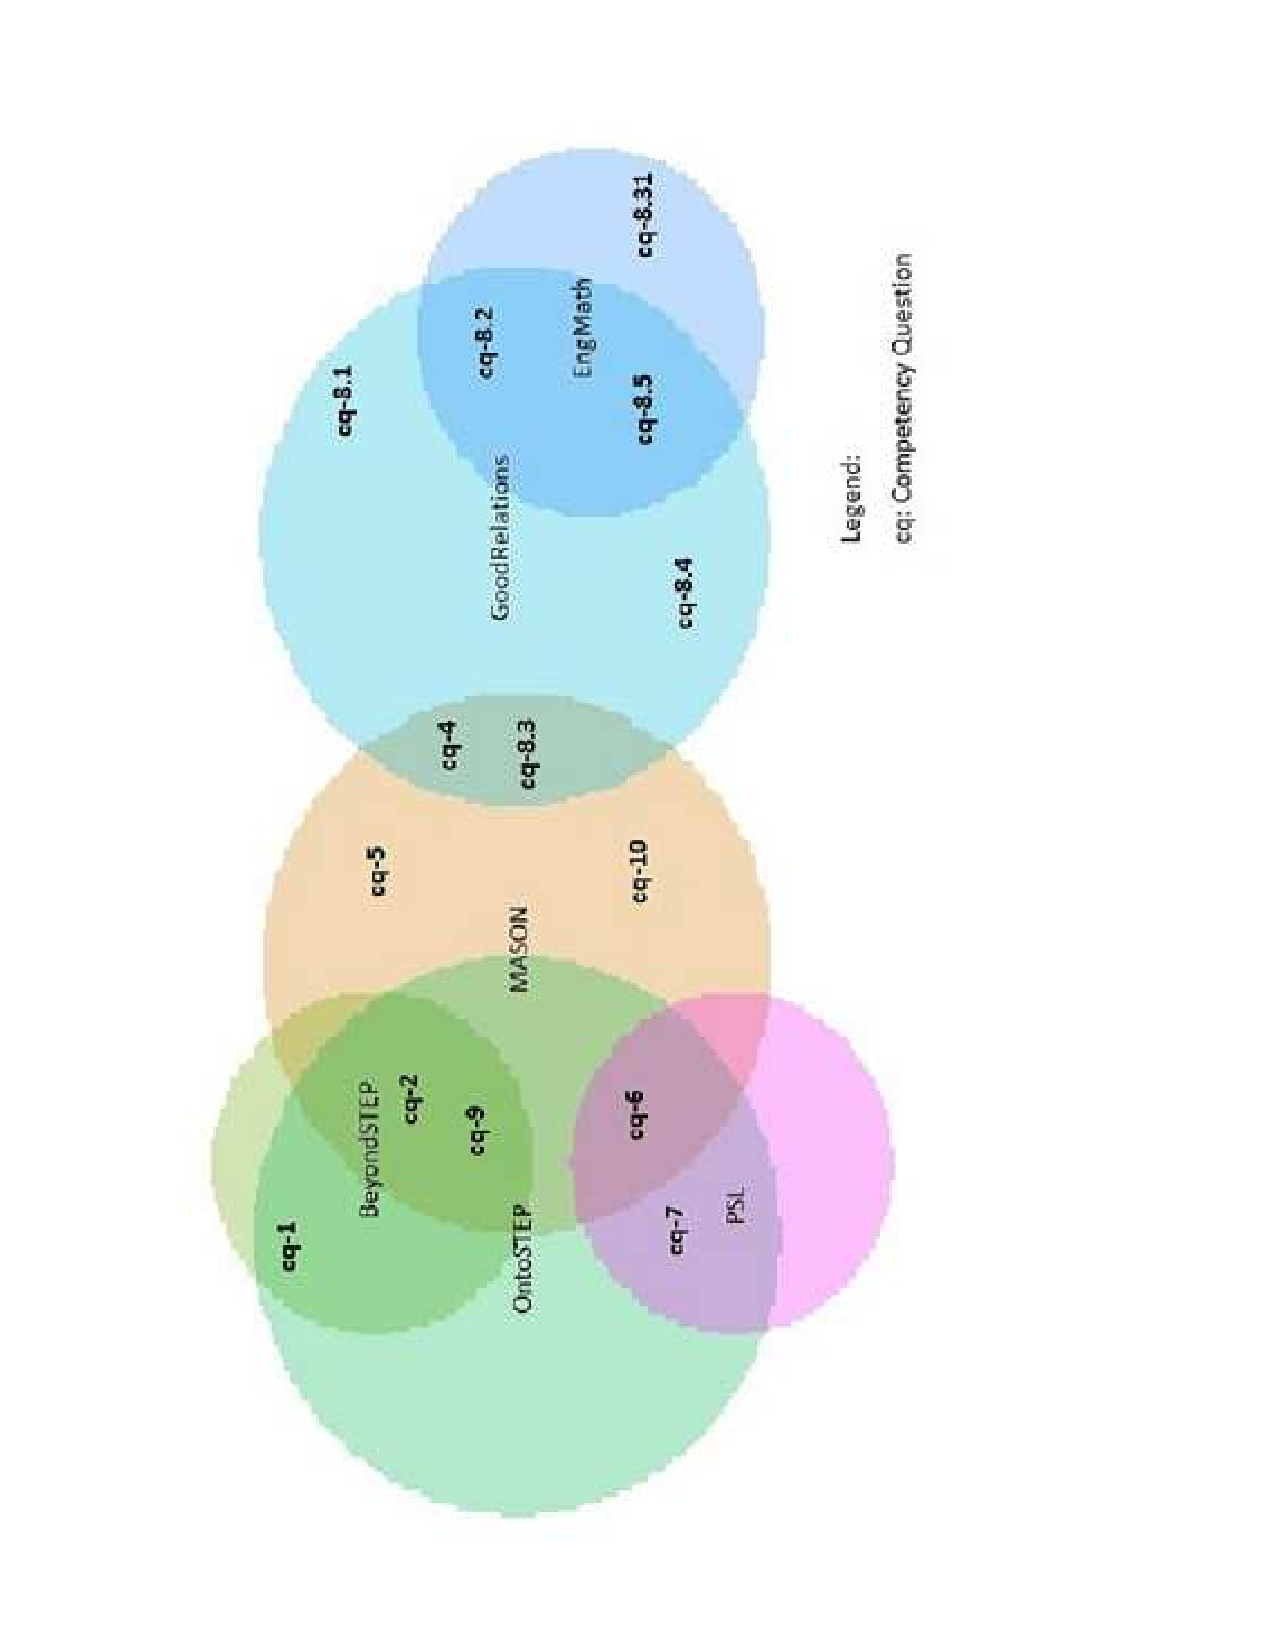
\includegraphics[scale=0.8]{figure-chapterIV/fig4-8}\\
		\caption{Ontological Commonalities in Answers to Competency Questions}
		\label{figure4-8}
	\end{center}
\end{figure}



Fig. \ref{figure4-8} represents another view of the scenario described in the previous paragraph. There, every circle represents one ontology and their overlapping regions indicate commonalities in answers to Competency Questions. The position of circles in this figure is also meaningful: from the middle to the left side, there are ontologies related to the products represented as solid   parts, and the manufacturing process representation as well. OntoSTEP nearly subsumes BeyondSTEP and PSL has commonalities with OntoSTEP and MASON, but not with BeyondSTEP. This occurs because BeyondSTEP does not mention any process in its terminology. On the right side of this figure is GoodRelation. This ontology is intended to represent products on the Internet, but it does not deal with representing manufacturing processes, therefore it is isolated from PSL. While it holds some relation with queries that can be answered by EngMath, given that the former highlights the use of International System  Units   in the definition of product features and parameters, which is wthin the scope of EngMath. \cbstart For instance, in the case of the cq-8.5 \textbf{What is the replacement cost?}, which is a query that comes from the fields of cost accounting, projects evaluation and insurance, concepts related to monetary units and physical units are required. Thus, for cq-8.5 the concepts \texttt{gr:UnitPriceSpecification}, \texttt{gr:QuantitativeValue} (GoodRelations), and \texttt{system-of-unit} (EngMath) can e considered to to provide an appropiate answer to this query\cbend. We can also mention that this result differs from what would be expected from ontologies for manufacturing and engineering science in general, given that metric units, the definition and concepts are fundamental in these fields. However, metric concepts do not appear in most of them.


In order to continue with this subject, and to provide sufficient generalization, it is beneficial to formalize the scenario described above with the following notions:


\begin{defn}\label{def4.10}
	A set of overlapping ontologies is a set of the form $O \equiv \{O_{1},O_{2},.., O_{n}\}$ where any ontology is of the form $O_{i} \equiv \{C,P,I\}$. If C, P and I corresponds to Concepts, Predicates and Instances, then 
	
	\forall \{(O_{i}, O_{j}) \in O \}_{i \neq j}
	
	the following conditions are fullfilled
	
	1. (C_{i} \cap C_{j}) \neq \varnothing
	
	and
	
	2. (C_{i} \neq C_{j})
	
\end{defn}



In this definition we consider that for any arbitrary set of ontologies, they are overlapping if there are two groups of concepts, those that are equal   to each other and those that are not for every pair of ontologies. Otherwise, we would be talking about isolated or redundant sets of ontologies.

Another notable aspect in our methodology is then to find ontologies that are able to provide answers to competency questions. This feature of ontology development was mentioned in Chapter \ref{chapter3}. It is expected to obtain answers to Competency Questions from the knowledge encoded in the ontology in the form of concepts or their instantiation. Moreover, methodologically speaking, we have finished the process depicted in Fig. \ref{figure3-1}, as soon as we find an ontology that provide answers to all the proposed Competency Questions, if any. This scenario is formalized below:



\begin{defn}\label{def4.2}
	
	Given an ontology $O$ as described in Subsection \ref{subsection2.2.1}, and a set of competency questions $CQ$, where  $CQ \equiv \{q_{1},q_{2},..,q_{n}\}$, both sets are related by means of an answer function $f$. This can be represented as follows:
	
	f = CQ \textrightarrow O 
	
	The assignment of the element $c_{1}$ of $O$ by f to an element $q_{1}$ of $CQ$ is denoted by
	
	f(q_{1}) = c_{1}
	
	We also can define the inverse function $f^{-1}(c_{n})$ which represent the set of elements of $O$ which correspond to answer of the queries in $CQ$, such definition is denoted as follows:
	
	f^{-1}(c_{n})= \{ q_{n} \in CQ \mid f(q_{n})=c_{n}\}
	
	
	Moreover, we have to consider the possibility that $O$ provides no answers to a given $q_{n}$ in $CQ$. Thus our $O$ set has to be modified as follows $\~{O} \equiv \{O, \phi \}$ where $\phi$ corresponds to the empty set, that means no answer to the query is provided. With this new set $\~{O}$ we can redefine our answer function $f$ as follows:
	
	f(q_{n}) =  \{$c_{n}$ if $f^{-1}(c_{n})= q_{n}$ \}
	
	$\phi$ if ther is not $c_{n} \in O$ that satisfies the function  $f^{-1}(c_{n}) = q_{n}$ 
	
	
	
\end{defn}




\begin{defn}\label{def4.3}
	
	Given a set of ontologies $O$, a set of competency questions $Q \equiv \{q_{1},q_{2},..,q_{n}\}$, and an answer function  defined as indicated in \ref{def4.2}, a fully reusable ontology $o_{r} \in O$ is that where:
	
	$\{\forall q_{n} \in CQ \mid  \exists c_j : f(q_{n} )=c_j \cap (c_j \in o_r )\}$
	
	\textbf{in words:} for all queries $q_{n}$ in CQ, exist a concept $c_j$ so that $f(q_{n} )=c_j∩$ ($c_j∩$ is the answer to this query $q_{n}$) and ($c_j$ belong to  $o_r$ )
\end{defn}


The definition above provides us with a mechanism to determine when ontology can be directly used in a given domain. That is when the ontology provides answers to every competency question. This kind of ontology is identified as $o_{r}$, and finding this type of ontology among a set of arbitrarily selected domain ontologies grants us the possibility of reusing it in the target domain. 

With the notions previously defined it is possible to introduce the next definition:

\begin{defn}\label{def4.4}
	(Modular Domain). Given a set of ontologies $O$, a set of competency questions $CQ$, and a function  $f(q_{n} )$, then a modular domain (D) is defined as follows:
	
	
	D=\{c_j\mid c_j \in o_x  \cap c_j \in o_y \cap f(q_{n} )=c_j\}
	
	\textbf{in words} a modular domain appears when an arbitrary concept $c_j$ is found as a member of at least two ontologies $o_x$ and $o_y$ and at the same time this concept $c_j$, satisfies the function $f(q_{n} )$. In other words, the concept $c_j$ is the answer to a CQ. 
\end{defn}


Example:  
\cbstart Assume that we have a set of overlapping ontologies $O \equiv \{o_{1},o_{2}\}$, where the sets of concepts $\{c_{1},c_{2},c_{3}\}$ \in $o_{1}$ and $\{c_{4},c_{5},c_{6}\} \in o_{2}$. If we accept that  $c_{1}=c_{4}$ and $c_{2} \neq c_{5}$, then the set  $O$ corresponds to a set of overlapping ontologies according to Definition \ref{def4.10}. Moreover, suppose that a set of queries exist $Q \equiv \{q_1,q_2,q_3 \}$ and an answer function $f(q_i )$, then a modular domain appears when answers to queries are distributed among ontologies. This fact is expressed as follows: $f(q_1 )=c_2$ and $f(q_2 )=c_5$ and $f(q_3 )=c_1=c_4$. \cbend

Definition \ref{def4.4} can be visualized in Fig \ref{figure4-8}, where a modular domain was obtained. 

In this case, considering the definitions presented above, and the results obtained until now, which are represented as the number of answer to queries (see Fig. \ref{figure4-6} and Fig. \ref{figure4-7} and its distribution in the network of ontologies  (see Fig. \ref{figure4-8}) we can proceed to summarize our findings in order to decide which way to  go from here:

\begin{enumerate}
	
	\item 	\cbstart First, according to the results outlined in Fig. \ref{figure4-6}, where we can see no ontology provides answers to every CQ, a fully reusable ontology $o_{r}$, as defined in Definition \ref{def4.3}, is not present in the manufacturing domain under study, and so a direct step to implementation is not possible for the given use case. \cbend  \label{it1} 
	
	\item Second, development from scratch should be discarded, given that the current manufacturing ontologies under consideration provide enough information to answer most of the domain questions  listed in Section \ref{4.1.2}, as we can observe in Fig. \ref{figure4-6}. Therefore, discarding these ontologies would make us lose time and other resources that could be used in developing a new ontology. \label{it2}
	
	\item Third, developing a new ontology with the ones evaluated as parts is another possibility. This ontology is also likely to use one of the existing ontologies as subsumed   and increase the knowledge encoded in the former by integrating the latter within it. \label{it3}
	
	\item Fourth, finding one ontology to be used as an interoperability artifact between a set of ontologies would make it necessary to determine whether an ontology exists that could be categorized as an upper level ontology. The use of this ontology should be similar to that displayed in Fig. \ref{figure2-1} (Chapter \ref{chapter2}), where one ontology is used with the sense of providing interoperability among domain ontologies. \label{it4}
	
	\item  Last, it is also possible to have separate ontologies that contribute to providing modeling structures and answers to queries distributed among subdomains.   For instance, a scenario like the one depicted in Fig. \ref{figure4-8}, where answer to queries are distributed among several ontologies.  \label{it5}
	
\end{enumerate}

Option \ref{it3} corresponds to the most common approach adopted in Ontological Engineering, that is: enriching an ontology by importing or merging other ontologies into it. Options \ref{it4} and \ref{it5} correspond to two schools of thought in Ontological Engineering, both of which were mentioned in Section \ref{section2.2} (Chapter \ref{chapter2}): the former corresponds to the upper level approach, and the latter corresponds to the hyper-ontological approach. In the next subsection these approaches, their implementations and issues within our domain of study are discussed.


\subsection{Mapping, merging and importing}\label{subsection4.2.4}

Mapping, merging and importing are some of the reutilization alternatives discussed in Ontological Engineering. \cbstart Mapping is particularly requiered for the task of modularity, which is hard to carry out automatically. \cbend The corresponding ontology editors who are implementing these techniques for reutilization were presented in detail in Table \ref{table2.1} in Chapter \ref{chapter2}. In this subsection, these techniques are implemented  for the selected ontologies listed previously in Table \ref{table4.2}  in order to clearly define which of the scenarios described at the end of the previous section we are facing. In other words, we have to determine if there is an upper level ontology, or if we have a network of ontologies, such as a hyperontology.

However, it is necessary to remark that these techniques are simple to implement when dealing with \textit{homogeneous} ontologies written in the same implementation language. In our case most ontologies presented in Table \ref{table4.2} are written in OWL. Consequently, there were only four ontologies available for immediate mapping of this type; these were MASON, the Beyond STEP Ontology, OntoSTEP and GoodRelations. The other high quality ontologies listed in Table \ref{table4.2}, PSL and EngMath, were not considered for automatic mapping because of its technological  limitation just mentioned, meaning that the ontology language of implementation differs from the language used in most high quality ontologies (OWL). 

According to the software tools listed in Table \ref{table2.1}, Protégé (prompt), Falcon and NeonToolKit are ontology editors that support OWL, thus they were chosen for mappings. Ontologies were mapped by pairs with every tool. The number of positive mappings were counted and tabled. Table \ref{table4.3} shows how this mapping experiment took place and which results were obtained by mapping the ontologies with different mapping tools and specific mapping techniques. In the third column mappings obtained by the PromptTab plug-in of Protégé are listed. In this case only mappings between a pair of ontologies were found. In the other cases, no mapping was found.  The mapping experiment was repeated with Falcon. In column four results mapping the target ontologies are listed. Experimenting with Falcon, mappings were found in only one of six cases. 

A third mapping experiment was carried out by the NeonToolKit Alignment plug-in. The fifth column of Table \ref{table4.3} lists every time an alignment was found with this tool.  This time, unlike the previous experiments, a positive mapping was found for each pair of ontologies in most cases. \cbstart There was a fundamental difference with this tool, that is we had the possibility to set up a similarity measure or threshold. Threshold of 1.0 would let us align only terms exactly written, a lower threshold value (e.g: 0.9, 0.8, 0.7) would let us aling similar terms like \texttt{paint} and \texttt{painting}, but a low threshold value (e.g: 0.3, 0.2) could drive have to obtain wrong alignments of term like \texttt{paint} and \texttt{point}. Thus, for our experiments we chose to set up a  threshold of 0.7. As a result, mappings provided by NeonToolKit were considered for further analysis. \cbend

Although a performance evaluation of mapping is not in the scope in this research, it is worth remarking that different results were obtained by applying the different alignment algorithms available in each software tool.  \cbstart NeOn alignment plug-in provided the best results, thus these results were taken for working out the modularity. \cbend



\begin{table}[tp]%
	
	\caption{Number of Ontology Mappings through Different Tools}
	\label{table4.3}\centering
	\begin{tabular}{p{2.5cm} p{2.5cm} p{2.5cm} p{2.5cm} p{2.5cm} }\toprule
		
		Ontology 1 &	Ontology 2	& Protégé 3.4.4 PromptTab*
		(Number of Alignments)	&Falcon-AO
		2010
		(Number of Alignments)	&NeonToolKit 2.3.1
		Alignment Plug in!
		(Number of Alignments) \\\toprule
		
		MASON &	BeyondSTEP&	18&	NaN	&34  \\\toprule
		MASON &	GoodRelations&	0&	NaN&	14 \\\toprule
		MASON	&OntoSTEP&	SC&	0,85&	101 \\\toprule
		BeyondSTEP&	OntoSTEP&	SC&	NaN&	209 \\\toprule
		BeyondSTEP&	GoodRelations&	0&	NaN	&21 \\\toprule
		OntoSTEP&	GoodRelations&	0&	NaN&	417 \\\toprule
		
	\end{tabular}
	\begin{flushleft}
		* With Lexical matching\\
		!SMOA Name Alignment and trim 0.7\\
		SC: System crashes \\
		NaN: No Alignment found\\
	\end{flushleft}
	
	
	
\end{table}

Mappings obtained with NeonToolKit (fifth column) were carefully checked manually in order to remove mappings that we considered incorrect, thus    false positive (FP) mappings produced by the mapping system were removed and only true positive (TP) mappings were included \citep{oliver_kutz_chinese_2010}. The cleaning process consisted in discarding every mapping falling in each of the following cases:

\begin{itemize}
	
	\item Property–property mappings were discarded.  
	
	\item \cbstart Redundant mapping through subsumption relations, in other words a concept in source mapped to two or more similar concepts in target. For instance, we obtained mappings  from \texttt{Bezier\_Curve} in source ontology to \texttt{Rational\_Bezier\_Curve} and \texttt{Bezier\_Curve} in the target ontology. That means, NeonToolKit provided two pairs of mappings: (\texttt{Rational} \texttt{\_Bezier} \texttt{\_Curve}, \texttt{Bezier\_Curve}) and (\texttt{Bezier\_Curve, Bezier\_Curve}). Thus, the first pair was discarded, and the second was considered. \cbend 
	
	\item Similar names, but with different meanings, e.g, mapping of \texttt{Paint} in source to \texttt{Point} in target, were discarded.
	
\end{itemize}


Furthermore, mapped concepts with a threshold lower than 1.0, but with similar meanings, were left in the mapping file, e.g., \texttt{Thread} in source mapped to \texttt{Threading} in target. Then, the total mappings were divided in FP and TP as depicted in Table \ref{table4.4}. The  output datasets corresponding to this experiment are available online (adding a link - I will publish the link before delivering the thesis).  


\begin{table}[tp]%
	
	\caption{Ontology Mapping in Manufacturing Domain (First Iteration)}
	\label{table4.4}\centering
	\begin{tabular}{p{2.5cm} p{2cm} p{2.5cm} p{1.5cm} p{1cm} p{1.5cm}}\toprule
		
		Ontology 1 & Concepts in source Ontology &	Ontology 2	& Number & of & Mappings
		
		\\\cline{4-6}
		
		&	&	& FP & TP & Total  \\\toprule
		MASON &	222 &	BeyondSTEP  &	27 &	7&	34 \\\toprule
		GoodRelations&	37&	MASON&	14&	0&	14 \\\toprule
		OntoSTEP &	1625&	MASON&	90&	11&	101 \\\toprule
		BeyondSTEP	&114&	OntoSTEP&	104	&105&	209 \\\toprule
		BeyondSTEP  &			-&	GoodRelations&	21	&0&	21 \\\toprule
		OntoSTEP&	-&	GoodRelations&	414&	3&	417\\\toprule
	\end{tabular}
	
\end{table}





Fig. \ref{figure4-9} shows a graphical representation of the TP mappings.  Only true positive mappings  between selected ontologies related to manufacturing are shown. This TP was selected according to the criterion previously described with the intention of avoiding incorrect mappings. For instance, mappings of similar terms with different meanings, like point and paint. Similar mappings were considered as FP and were discarded. In the figure, we can observe that the number of mappings from BeyondSTEP to OntoSTEP (105) appears to be the most significant one in this set of ontologies, but when the number of concepts of Beyond STEP (114) were considered, and compared against the number of TP mappings, it can be observed that more than 92\% of the concepts in BeyondSTEP were present in OntoSTEP. This result shows a scenario similar to the one shown in Fig. \ref{figure3-2}, where BeyondSTEP was mostly subsumed by OntoSTEP.  


\begin{figure}
	\begin{center}
		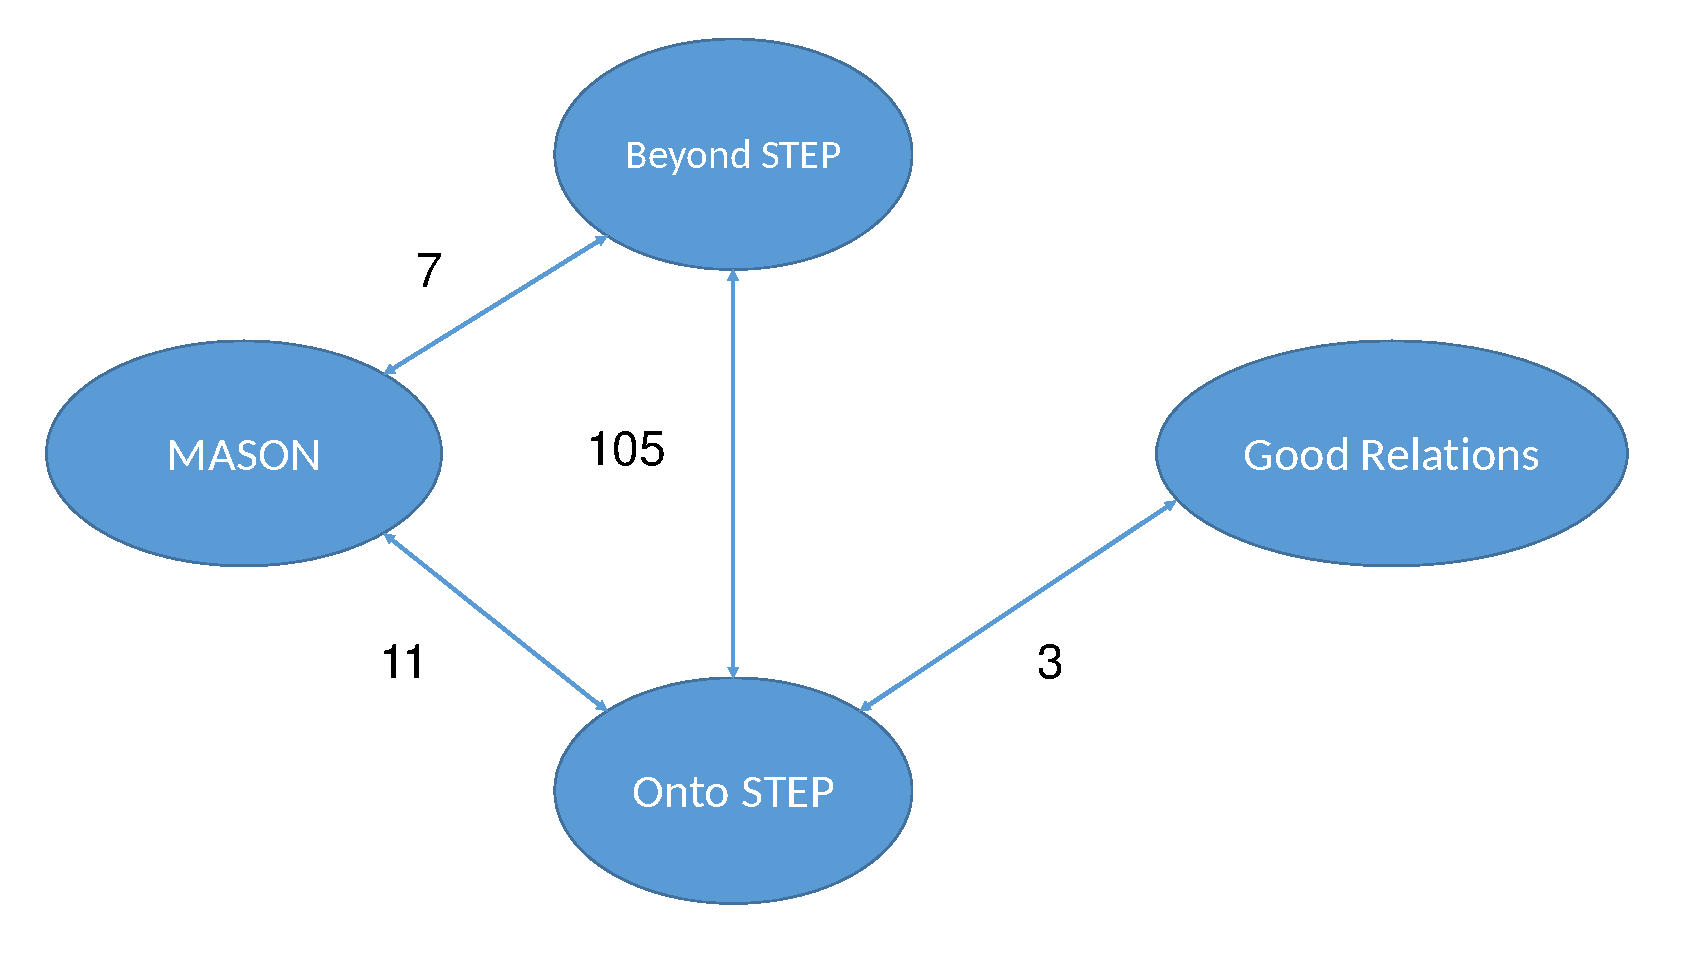
\includegraphics[scale=0.5]{figure-chapterIV/fig4-9}\\
		\caption{Ontological Commonalities in Answers to Competency Questions}
		\label{figure4-9}
	\end{center}
\end{figure}



However, when mappings are reviewed in detail, we find that both BeyondSTEP and OntoSTEP share some common mappings with MASON. These are the ones related to geometric concepts. Also, the mappings MASON-OntoSTEP highlight mechanical feature concepts on the one hand, while on the other hand the mappings   MASON-BeyondSTEP highlight more complex geometric concepts. This mapping situation shows a very common scenario in Ontological Engineering, i.e., the existence of    overlapping ontologies $O_{1}$ and $O_{2}$ which describe independent aspects of a given domain, but with some overlap. 

As our interest consists in finding answers to the competency questions previously listed, a first method would be to grant full access to the knowledge in those ontologies in order to answer these domain questions. This is equivalent to integrating them by merging. To proceed with this, Protégé 4 was selected from Table \ref{table2.1} as an ontology editor implementing support for merging ontologies. Thus, MASON and OntoSTEP were merged first, obtaining a new ontology. However, after merging them and running the respecitve reasoner, it was found that the resulting ontology wbecame inconsistent.

Much has been studied about the issue   of inconsistency for ontology reutilization. For instance, \cite{ghilardi_did_2006} show that the appearance of inconsistencies when merging ontologies also depends on the logic of the ontology language in which the ontologies to be merged are implemented, in other words if we have two ontologies, one written in OWL, and another written in FOL, they cannot be merged, because of the language hetereogenity. To date some techniques to deal with inconsistent scenarios have been proposed by \citet{grau_owl_2008}  and \citet{xiang_ontofox:_2010}; both authors considered the need for user intervention and judgment in order to extract those modules from  $O_{1}$ which can be reused in $O_{2}$ avoiding inconsistencies. Others  authors have recommended keeping ontologies separated, but with logical links among these ontologies (e.g \citet{bateman_oasis_2009} and \citet{kutz_carnap_2010}). 

However, from the options given above, those considering human intervention are only feasible when dealing with pairs of small ontologies. In cases where a larger number of ontologies with a larger number of concepts are present, the implementation of appropriate algorithms for generating candidate modules is clearly going to be necessary as long as this proves possible.  Thus, the human intervention possibility is discarded here. Before considering the last posibility  (option \ref{it5}, of the list depicted in Subsection \ref{subsection4.2.3}, that is the  hyper-ontology), we exhausted option \ref{it4}: that is the possibility of finding one ontology of Upper Level as an interoperability artifact. Therefore, retaking Fig. \ref{figure3-1} where our methodology is described, we  decided on Reusability, because we found evidence that the ontologies under study (see Table \ref{table4.1}), provide answers to some of the Competency Questions proposed, that means we are in a Multiontology environment. Then, we have to evaluate the most commonly found approach in Ontological Engineering, which is using an ontology as an interoperability artifact among other ontologies. That means that  we have to determine if one of the ontologies under study could receive  a higher categorization of upper level.   

In this vein the number of mappings in Fig. \ref{figure4-9} is insufficient to make any conclusions, because most of the mappings are inconsistent in number, and similarly directed to one ontology or distributed among ontologies. Therefore, a second mapping iteration   was carried out in order to obtain a larger network mapping, and obtain more accurate conclusions. 

According to the quality order previously outlined in Table \ref{table4.2}, the SWOP Product Ontology, SWEET Units, PRONTO and ONTOMoPS were considered for this second iteration. In this case, only NeonToolKit was used for further experiences because of the better performance shown in the results obtained from Table \ref{table4.3} from the previous iteration. 

Fig. \ref{figure4-10} represents the output of including the mappings of this second iteration of ontologies. Here, OntoSTEP appears to also have the most mapping sets to every ontology in this network and BeyondStep has six mappings, while SWOP and OntoMoPs have five mappings respectively.  It is worth highlighting that these last two ontologies were not considered for the first iteration because of their lower quality evaluation. However with an automatic tool like NeonTooloKit we have found they have a large set of commonalities in the network of ontologies evaluated. The terms: \texttt{Product, Unit, Assembly, Process} and \texttt{Material} were some of those common terms found. \cbstart  SWOP and OntoMoPs were discarded at the begining because of preliminar evaluations, that did not consider the encoded knowledge in a first step. Those previous evaluation are ilustrated in Fig. \ref{figure4-1} and Fig. \ref{figure4-6}. Nevertheless, at this stage an automatic tool was included, taking us to discard others and retake these ontologies. \cbend




\begin{figure}
	\begin{center}
		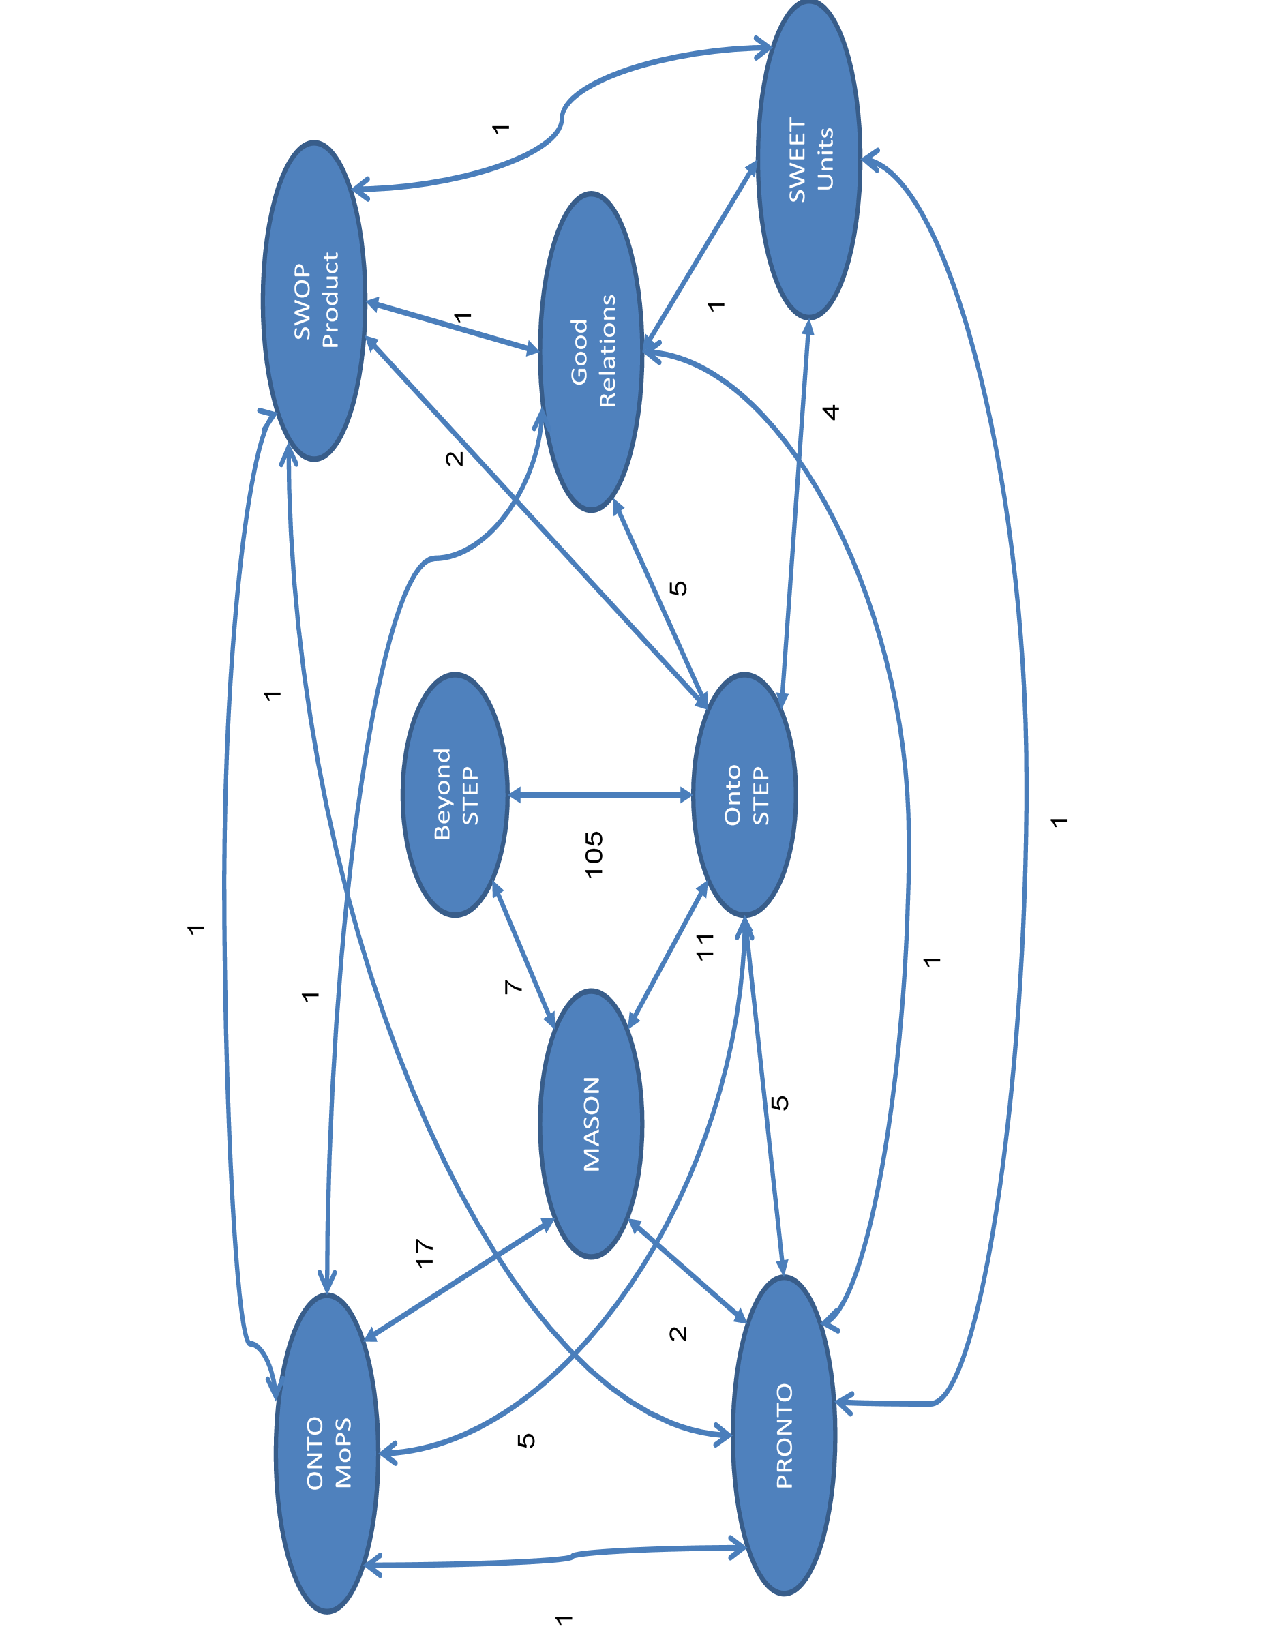
\includegraphics[scale=0.8]{figure-chapterIV/fig4-10}\\
		\caption{Network of Mappings in Manufacturing Ontologies}
		\label{figure4-10}
	\end{center}
\end{figure}



In the specific case of the set of mappings between BeyondSTEP and OntoSTEP, this large set of mappings was expected due to both ontologies having a closely related scope, which is the STEP standard. Although slightly different in the parts of the standard they modeled, the relation among the number of true positive mappings and the number of concepts of BeyondSTEP (92.1\%) allows us to affirm that BeyondSTEP is redundant compared to OntoSTEP.

Discarding the set of mappings between BeyondSTEP and OntoSTEP, a more complex scenario was obtained.  In this case, from the 28 mappings 19 were sets of true positive mappings ranging from only one (7 times) to 16 individual mappings. The sets of only one mapping contained the terms Product and/or Unit. The remainder sets contained terms related to geometry features of products, mechanical features, and other terms repeated less frequently, such as assembly, material and process. Table \ref{table4.5} presents the details of those terms and their frequency. Here we can retake the list of terms we mentioned in Section \ref{4.2.1}, proposed by \cite{martin_design_2003} and \cite{lastra_ontologies_2009} as significant for the manufacturing domain. Those  are \texttt{Product}, \texttt{Process}, \texttt{Resource} and \texttt{Equipment}. All of them except \textbf{Equipment} are present in this table. The obtained mapping terminology was grouped according to the proposal of the mentioned authors. For instance, the terms \texttt{Assembly}, \texttt{Part} and \texttt{Set} were considered as representations of \texttt{Product}. Likewise the terms \texttt{Operation, Change, Transformation, Milling} and \texttt{Drilling}, were grouped as \texttt{Process}. 


There are two additional aspects to comment from this table. At first they appeared as new terms that can be considered significant as well. Those that were grouped as features, which included specific mechanical features, were obtained by machining process, and the other term was Unit. This last term was not grouped with other mappings, however it presents the most frequent after the term \texttt{Product}. Consequently this term has to be considered as significant as the ones proposed by the authors mentioned above.


\begin{table}[tp]%
	
	\caption{Ontology Mapping in Manufacturing Domain (First Iteration)}
	\label{table4.5}\centering
	\begin{tabular}{p{2.5cm} p{2cm} p{2.5cm}}\toprule
		
		Terms 1 &	Mapping Frequency	& Grouping \\\toprule
		Product	&7&	Product\\\toprule
		Assembly&	3&	Product\\\toprule
		Part&	1&	Product\\\toprule
		Set&	1&	Product\\\toprule
		Circular Slot&	2&	Features\\\toprule
		chamfer&	1&	Features\\\toprule
		slot&	1&	Features\\\toprule
		pocket&	1	&Features\\\toprule
		Line&	2&	Features\\\toprule
		Operation&	1&	Process\\\toprule
		change&	1&	Process\\\toprule
		Transformation&	1&	Process\\\toprule
		Process	&1&	Process\\\toprule
		Milling&	1&	Process\\\toprule
		Drilling&	1&	Process\\\toprule
		Event&	1&	Process\\\toprule
		Resource&	1&	Resource\\\toprule
		Tool&	1&	Resource\\\toprule
		Machine	&1&	Resource\\\toprule
		Lathe&	1&	Resource\\\toprule
		Organization&	1&	Resource\\\toprule
		Person&	1&	Resource\\\toprule
		Material&	2&	Resource\\\toprule
		Unit&	6&	Unit\\\toprule
		
		
	\end{tabular}
	
\end{table}



We consider that because of the number of mappings shown in Fig. \ref{figure4-10}, which is larger than the number of mappings shown Fig. \ref{figure4-9}, we had to continue working with the network of ontologies shown in the later. 

Of course, it is necessary to remember that our goal is to determine whether or not in this network we can identify one of the following patterns:

\begin{itemize}
	\item[a] An ontology that could be used as an interoperability artifact between other ontologies, or
	\item[b] Ontologies that could be used as separate modules in a network of ontologies. 
\end{itemize}


Here we observe the issue that, besides having a network with significant terms, to date there is no systematic and objective procedure to determine   when an ontology can be   considered as upper level. Moreover, as we indicated in Section \ref{subsection2.4.3}, some authors have proposed their manufacturing ontologies as ULO, without providing a proper reason, analysis or methodology to support such a statement. Therefore, it is necessary to accurately define when an ontology is “Upper Level”. We support such a definition in Fig. \ref{figure4-12}. There we can observe that there is an $O_{u}$ that serves as an interoperability artifact between $O_{s}$ and $O_{t}$. Exchange of information occurs from $C_{s}$ to $C_{t}$ or vice versa, but always using the $C_{u}$. $C_{u}$ is present in $O_{u}$, which is actually the  upper level ontology. The red dashed lines correspond to mappings, and the blue dash lines correspond to “is a” arcs (See Section \ref{subsection2.2.1} in Chapter \ref{chapter2}). Finally, the figure presents a “Deployment” dimension. This “Deployment” indicates how the mapped concept deploys itself among the source or target ontology. 



\begin{figure}
	\begin{center}
		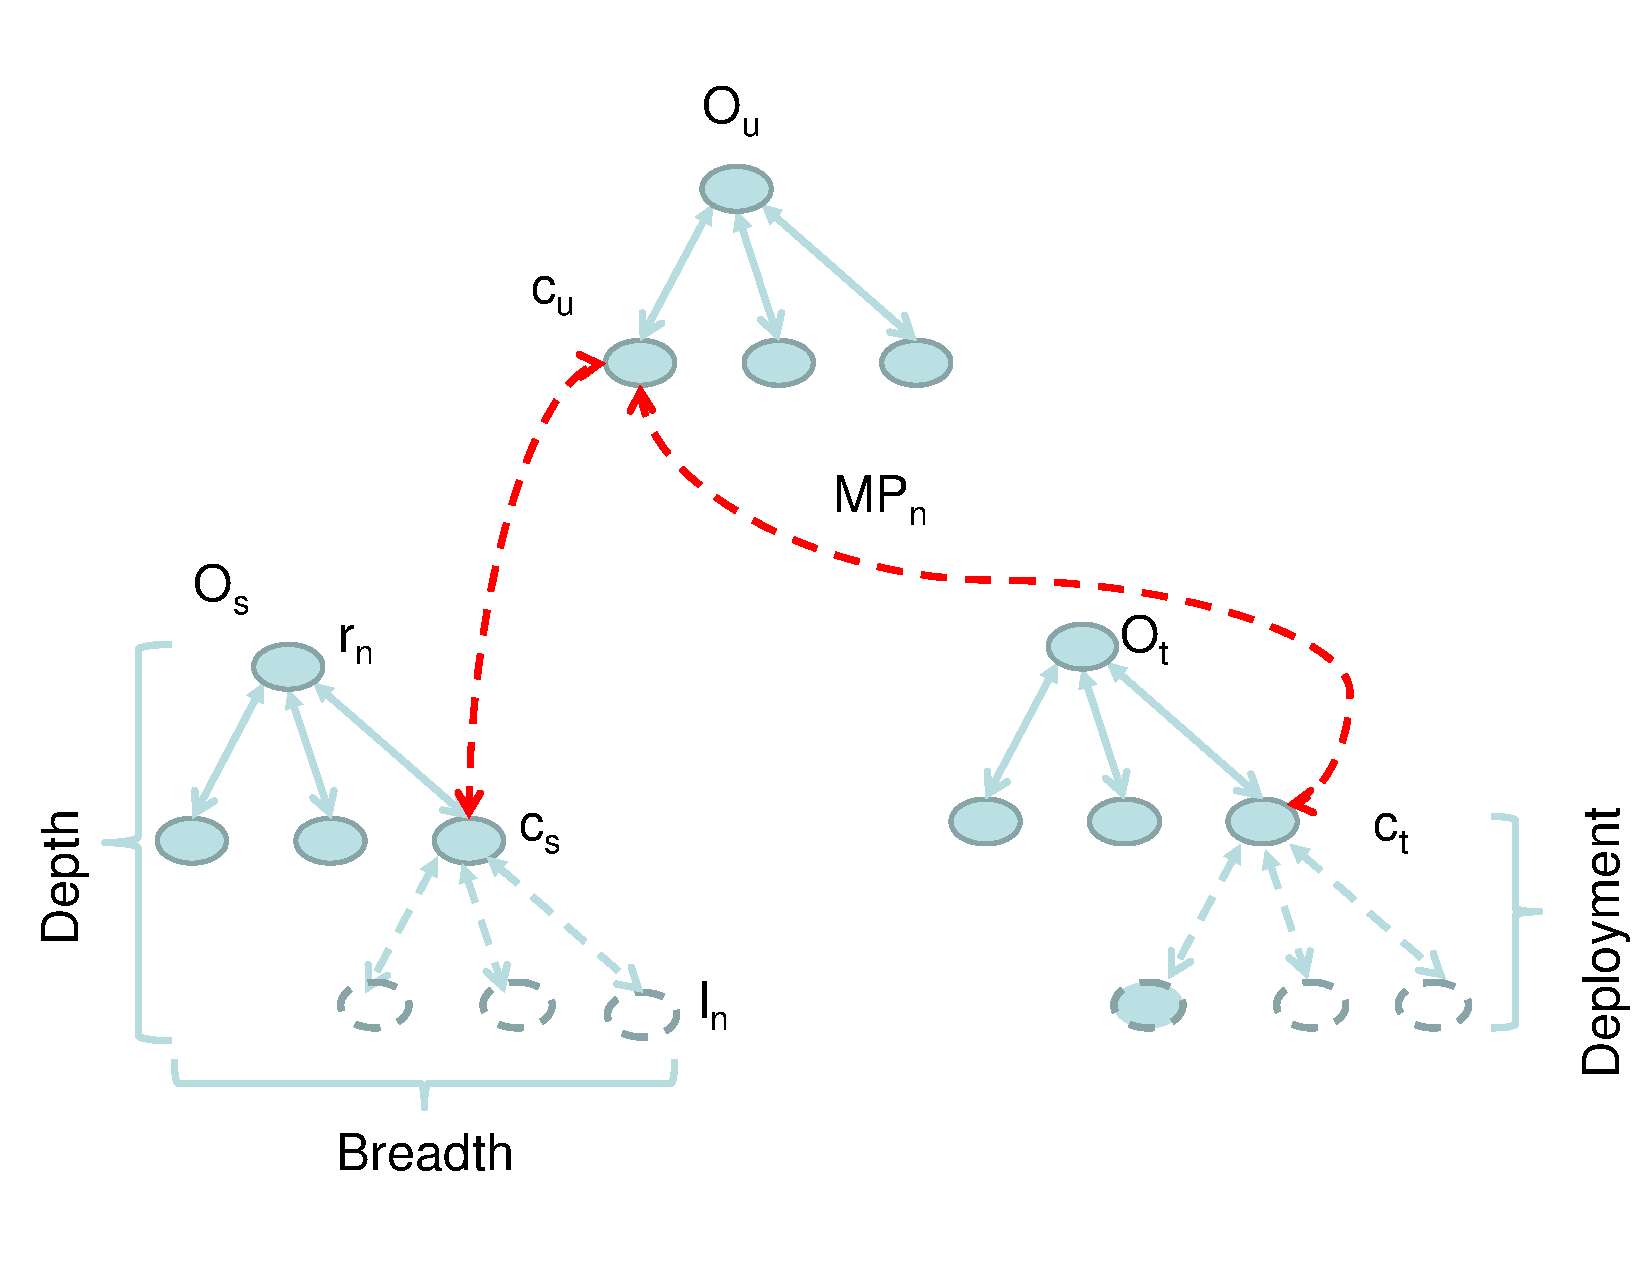
\includegraphics[scale=0.6, angle=90]{figure-chapterIV/fig4-11.pdf}\\
		\caption{Relative Upper Ontology}
		\label{figure4-11}
	\end{center}
\end{figure}



But, besides having graphically characterized an ontology of Upper Level through Fig. \ref{figure4-12}, when compared to Fig. \ref{figure4-11}, it is not possible to conclude which ontology should be considered as upper to the others. That occurs because the mappings are not directed to a single ontology, which could be identified at first sight, but most ontologies have mappings with each other without making any pattern evident. Conversely, the ontologies present a minimum of two mapping ranging to seven mappings. Consequently, in order determine whether or not such a pattern exists we propose a graphical structural analysis similar to that proposed by \cite{gangemi_modelling_2006}.  Thus, the following measurement function M was implemented:

\begin{equation}
	$
	M=〈D,S,mp〉
	$
\end{equation}

\

Where:

$\langle D \rangle =Dimension$ is the graph property   we want  to measure, e.g depth, breath or deployment. 

$ \langle S_{x} \rangle $ $=$ $Set$ $ of $ $ graph$ $ element$s is the collection of elements  in the $x$ graph, those elements correspond to nodes or arc. In ontology, these elements can define instances or “is a” arcs.  $x$ corresponds to the type of graph   or ontology we are considering, these graphics can be source, upper or target ontology. 

$ \langle mp \rangle $ $=$ $Measurement$ $ procedure$ is the procedure followed to perform the measurement of the given dimension. 


When applying a measurement procedure $mp$ to obtain a value of the dimension $D$ over a set $S$ of graph elements, with a given coefficient $c$, we obtain  the  value of M:

\begin{equation}
	mp_{D,S}   \longrightarrow  m   \in R 
\end{equation}


In contrast to the approach of Gangemi et al, \cbstart which was proposed for the evaluation of inividual ontologies, we define several measurement sets according to the context depicted in Fig. \ref{figure4-11}. That is a multiontology environment from where several modules can be obtained. Those sets were:\cbend 


\begin{itemize}
	\item 	The set of upper nodes $C〗_{u} $ \in  $O_{u} $, where upper nodes are those concepts of the upper ontology that are  mapped to $C〗_{s} $ \in  $O_{s} $ in the source ontology and  $C〗_{t} $ \in  $O_{t} $, in the target ontology.
	
	\item 	The set of source nodes $C〗_{s} $ \in  $O_{s} $, where source nodes correspond to those which are  mapped to a set of upper nodes in $O_{u}$. 
	
	\item 	The set of target nodes $C〗_{t} $ \in  $O_{t} $, where target nodes correspond to those which have positive mappings  to a set of upper nodes of $O_{u}$. 
	
	\item 	The set of deployed nodes $DEPC_{j \in O{x}}$, connected to the same positive mapped node $C_{j}$ in an ontology $O$, which can be source, target or upper ontology.
	
	\item 	The set of mappings $MP$ where $MP$ groups sequences of directly mapped concepts from independent ontologies starting in the source concept  $C〗_{u} $ \in  $O_{u} $ and ending in a target concept〖 $C〗_{t} $ \in  $O_{t} $. 
	
	\item 	The set of deployment levels $LD$, where a deployment level is measured from a mapped  concept, either source, target or upper concept to the leaf concept. That is, the number of branches that start in the mapped concept and end in the leaf concept. In Fig. \ref{figure4-12} we found only one deployment level in 〖$C_{t} $ and  $C_{s}$, while $C_{u}$ has no deployment level. 
	
\end{itemize}

With the definition of the terminology depicted above, we can proceed to propose the following metrics in order to determine when an ontology is upper level. 

\begin{enumerate}
	\item Deployment Measures:
	This metric is ilustrated in \ref{figure4-12}. It indicates how new concepts derive from a mapped concept   which serves as root, either source, target or upper ontology. This measurement provides a numeric relation between the number of mappings present in the ontology, and the number of concepts that are derived from the mapped concept which serves as root. This indicates how many newer concepts arise among mappings, giving us an idea of growth within the mapping instances. 
	
	The following were the deployment measures used in our evaluation:
	
	\item Average $C_{x}$ Deployment:
	
	
	\begin{equation}\label{eq.4.5}
		ADC_{x} = \frac{1}{N_{MP(C_{x})}} \sum_{j=1}^{N_{MP(C_{x})}} DEPC_{j} \in O_{x}
	\end{equation}
	
	Where $O_{x}$ corresponds to the kind of ontology, either source, upper or target, $C_{x}$ refers to a given concept in one of those graphs or ontologies, and ${N_{MP(C_{x})}}$ represents to the numbers of mappings from source to target ontologies. In  Fig. \ref{figure4-12} We provide an example of this metric, there are 2 ontologies ($O_{x_{1}}$ and $O_{x_{2}}$)  mapped to an Upper ontology $O_{u}$. The mapping obtains one concept in each ontology, both ontologies are identified with an “$x$” subscript because ontology can be a source or a target. There are also 2 sets of deployed nodes, those are $DEPC_{1}$ and $DEPC_{2}$.
	
	
	
	\begin{figure}
		\begin{center}
			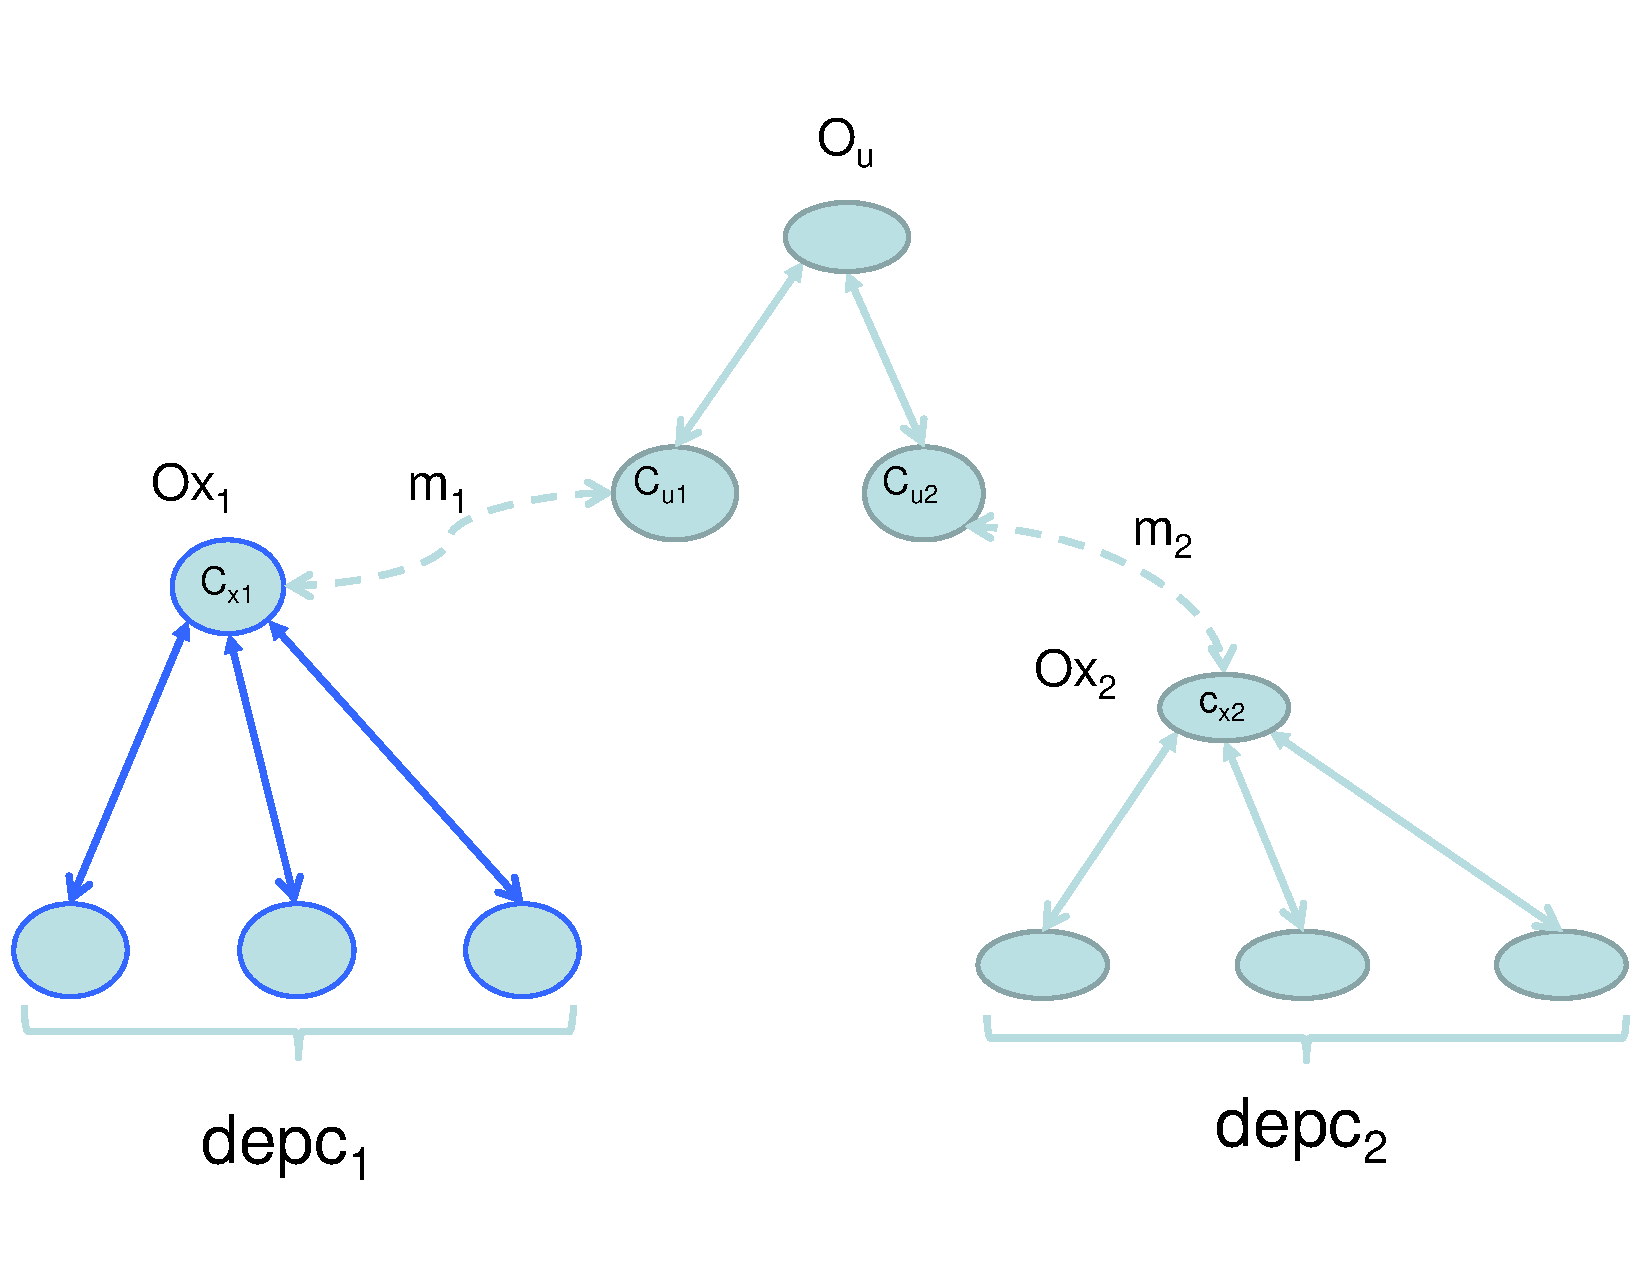
\includegraphics[scale=0.6, angle=90]{figure-chapterIV/fig4-12.pdf}\\
			\caption{Average $C_{x}$ Deployment}
			\label{figure4-12}
		\end{center}
	\end{figure}
	
	
	
	
	Besides obtaining a relation between deployed nodes and mapping, we also considered it necessary to measure the average of deployed nodes starting from the mapped concept $C_{x}$ in source or target ontology. For this we introduce the following metric:
	
	
	\item Average Source, Target:
	
	\begin{equation}\label{eq.4.6}
		AST =  \frac{|MC_1|+|MC_2|}{2} \in O{x}
	\end{equation}
	
	Where AST provides the average of mappings distributed among source and target ontology for a given upper ontology. Moreover, $|MC_1|$ corresponds to the number of mapped concepts in source or target ontology. 
	
	
\end{enumerate}


\noindent With the definition of the previous metrics, we calculated the results for the adopted ontologies, and  display the results in Fig. \ref{figure4-13}. 

\begin{figure}
	\begin{center}
		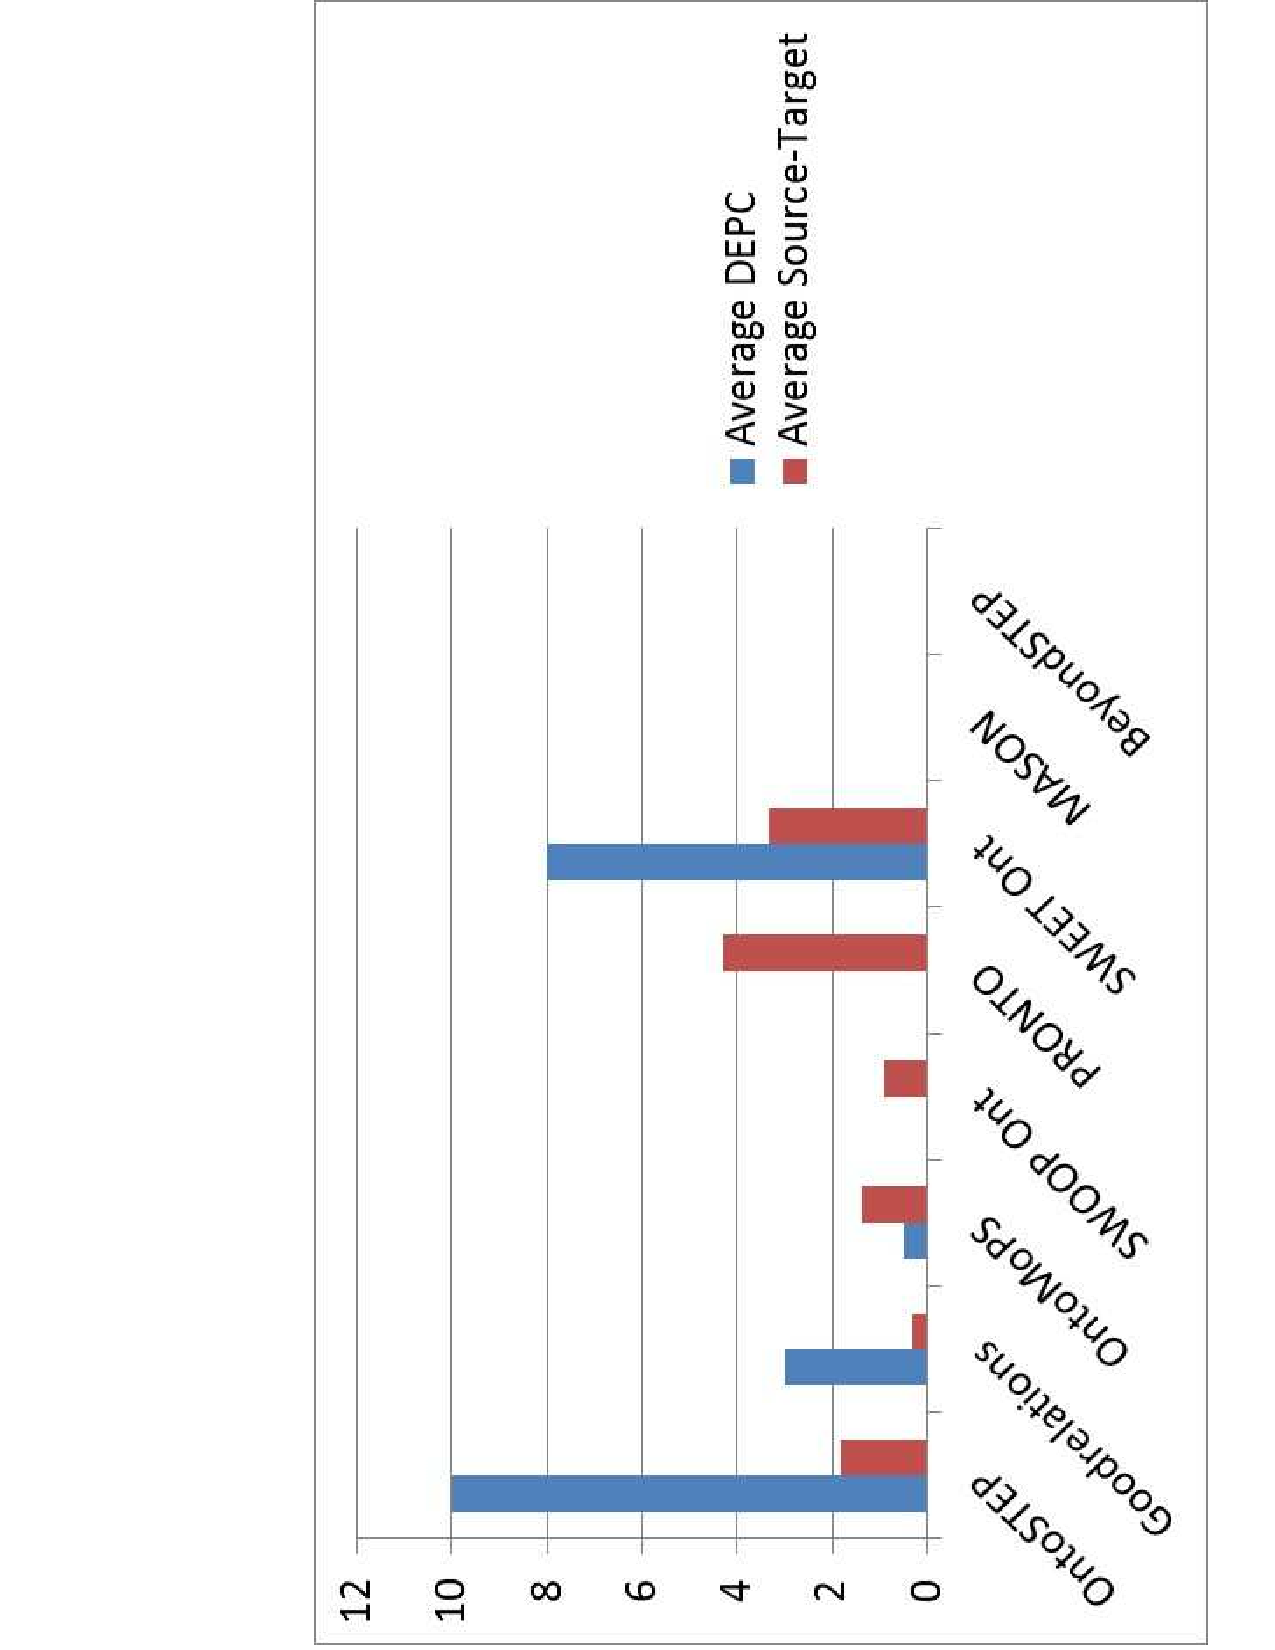
\includegraphics[scale=0.5, angle=-90]{figure-chapterIV/fig4-13.pdf}\\
		\caption{Relative Upper Relationship among Ontologies}
		\label{figure4-13}
	\end{center}
\end{figure}



As we stated in the previous paragraphs, when the concept of deployment measurement  was introduced, this evaluation is intended to determine: first how an upper ontology is compared to other pairs of ontologies that have mappings among them and, second, the interoperability level  that could be provided by this ontology in a hypothetical network of systems where the other ontologies are implemented. For authors like \cite{borgo_role_2004}, this interoperability is granted by means of shared ontologies, but while they provide a subjective method for alignment of ULO´s with manufacturing ontologies, and other authors like \cite{lemaignan_mason:_2006} declare their manufacturing ontologies as ULO´s without providing enough support for such a statement, we consider that more objective metrics are required. In this vein the figure depicted above breaks down how the results were obtained applying the metrics to the network of ontologies shown in Fig. \ref{figure4-10}. That is, the upper relationship between ontology and its respective mapping environment. Unlike the previous  views provided in Fig. \ref{figure4-9} and Fig. \ref{figure4-10}, with the results depicted in Fig. \ref{figure4-13}, we have a criterion to determine how upper an ontology is compared to others in a network. 


Fig. \ref{figure4-10} introduced above is interpreted as follows: Every ontology evaluation yields two columns. The left column corresponds to the average of  deployment of concepts among the ontology evaluated as an upper one, and the right column corresponds to the  average of mapped   concepts in the source and the target ontology. To consider one of the evaluated ontologies as relatively upper in comparison to the others within the network under study, the two following assumptions are made:

\begin{itemize}
	\item [a] The column on the left should be smaller than the column on the right for the ontology under evaluation. When this occurs, it means that the deployment of mapped concepts in source and target ontologies is larger than the deployment in the upper ontology.
	
	\item [b] The column on the left is greater than 2. This value for the source and target indicates that for each mapping concept at least two new concepts are linked to it by arcs. This means that, as in the previous points, the mapped concept has been deployed in the source and target ontologies, and that it is not a mapping with a leaf node.
	
\end{itemize}

According to the criterion indicated above, and considering the results depicted in Fig. \ref{figure4-13}, we can mention that in the manufacturing network of ontologies shown in Fig. \ref{figure4-10} there is a lack of any single ontology that could be considered to occupy a relatively upper level in the network. In other words, according to our metrics, none of the manufacturing ontologies evaluated would serve as an interoperability artifact among other ontologies. 

The relevance of this discussion on the presence of ULO´s in the network of ontologies presented in Fig. \ref{figure4-11} lies on one hand in the fact that some of the ontologies presented used in this evaluation have been declared as ULO´s by their proponents without supporting   their statements in a detailed analysis of previously existing ontologies in the domain. MASON and SWOP are some of these Upper Levels Ontologies. On the other   hand, although the concept of ULO is clearly defined from the philosophical point of view and many ULO´s are clearly identified, the category of ontologies according to the hierarchy indicated in Fig. \ref{figure2-1}  is still subjective. This issue may cause interoperability misinterpretations when using an ontology in a hierarchy higher than where it should be according to its \textit{ontological contribution} to the given target domain, manufacturing in our case. Consequently, with this partial result of our research, in Fig. \ref{figure4-13} we highlight the necessity of evaluation of ontologies in a given network of ontologies  prior to declaring them as Upper Level Ontologies. If we declared ontology to be upper level for a given domain, to our knowledge it means it can be used to enable interoperability between systems that use lower level ontologies. This “level” of the ontology is not related to quality, but with reusability according to Fig. \ref{figure2-1}. This means the more, \textit{upper the ontology} the more reusable it is, because it is more general, however the upper is the ontology the less usable it is, which is a disadvantage. Therefore, Ontological engineers shall be able to manage such a categorization. 

From our point of view, what some authors have tried to express when declaring their ontologies as ULO´s, is that they assume their ontologies have a higher level of reusability than the other ontologies they compared in their studies. Such a feature would make their ontologies more reusable, but according to our evaluation it is not simple to highlight one of the evaluated ontologies for permitting interoperability among the others. 

Because it was not possible to find the ontology category of Upper Level in the evaluated network. In the following subsection, we will proceed to describe the next steps of our methodology    (see Fig. \ref{figure3-1} in Chapter \ref{chapter3}) in order to determine whether or not it is possible to establish other kinds of relations between those manufacturing ontologies. 

\subsection{Hyper Modules Extraction}\label{subsection4.2.5}

As discussed in Subsection \ref{subsection2.2.6} (Chapter \ref{chapter2}) and Subsection \ref{section3.1} (Chapter \ref{chapter3}), modularity can be pursued as an alternative to the ULO approach, intended to enable maintenance, publication, validation and processing of ontologies \citep{daquin_modular_2009}. Two main modularity approaches have been distinguished from each other in the literature, the former corresponds to the division of a large ontology into modules, thus rendering such an ontology to be more manageable, and the latter corresponds to the generation of small modules from links between some collections of ontologies in an storage.  Defining so-called ‘hyperlinks’ between ontologies is intended to enable the interconnection of    related ontologies, but without merging the logical content of those ontologies. This last approach was introduced above  as \textit{Hyperontology} in Subsection \ref{subsection2.2.1} (Chapter \ref{chapter2}). 

In addition to mappings between concepts that are considered equivalent, which is the foundation of hyperontological networks, we argue that the identification and consideration of subsumption relations   between equivalent concepts in this hyperontology will allow us to identify \textit{hypermodules}. 

We define Hyper modules as identified sets of concepts that constitute commonalities in a network of ontologies. Acording to Fig. \ref{figure4-14}, given a network of ontologies $O_{1}$, $O_{2}}$, $O_{n}$, a hypermodule is bounded by mapped  root concepts ($C_{r}$) and a set of mapped leaf concepts ($C_{1}$), which are connected by subsumption arcs, providing a path from root to leaf concepts. Then the  concepts involved in such hypermodules are those with  mappings  ($m_{1}$, $m_{2}$, $m_{3}$, $m_{n}$) and the quality of such modules is given by the number of mapped concepts and the distance ($d_{i,j}$) that separates root and leaf concepts. \textbf{why?}



\begin{figure}
\begin{center}
	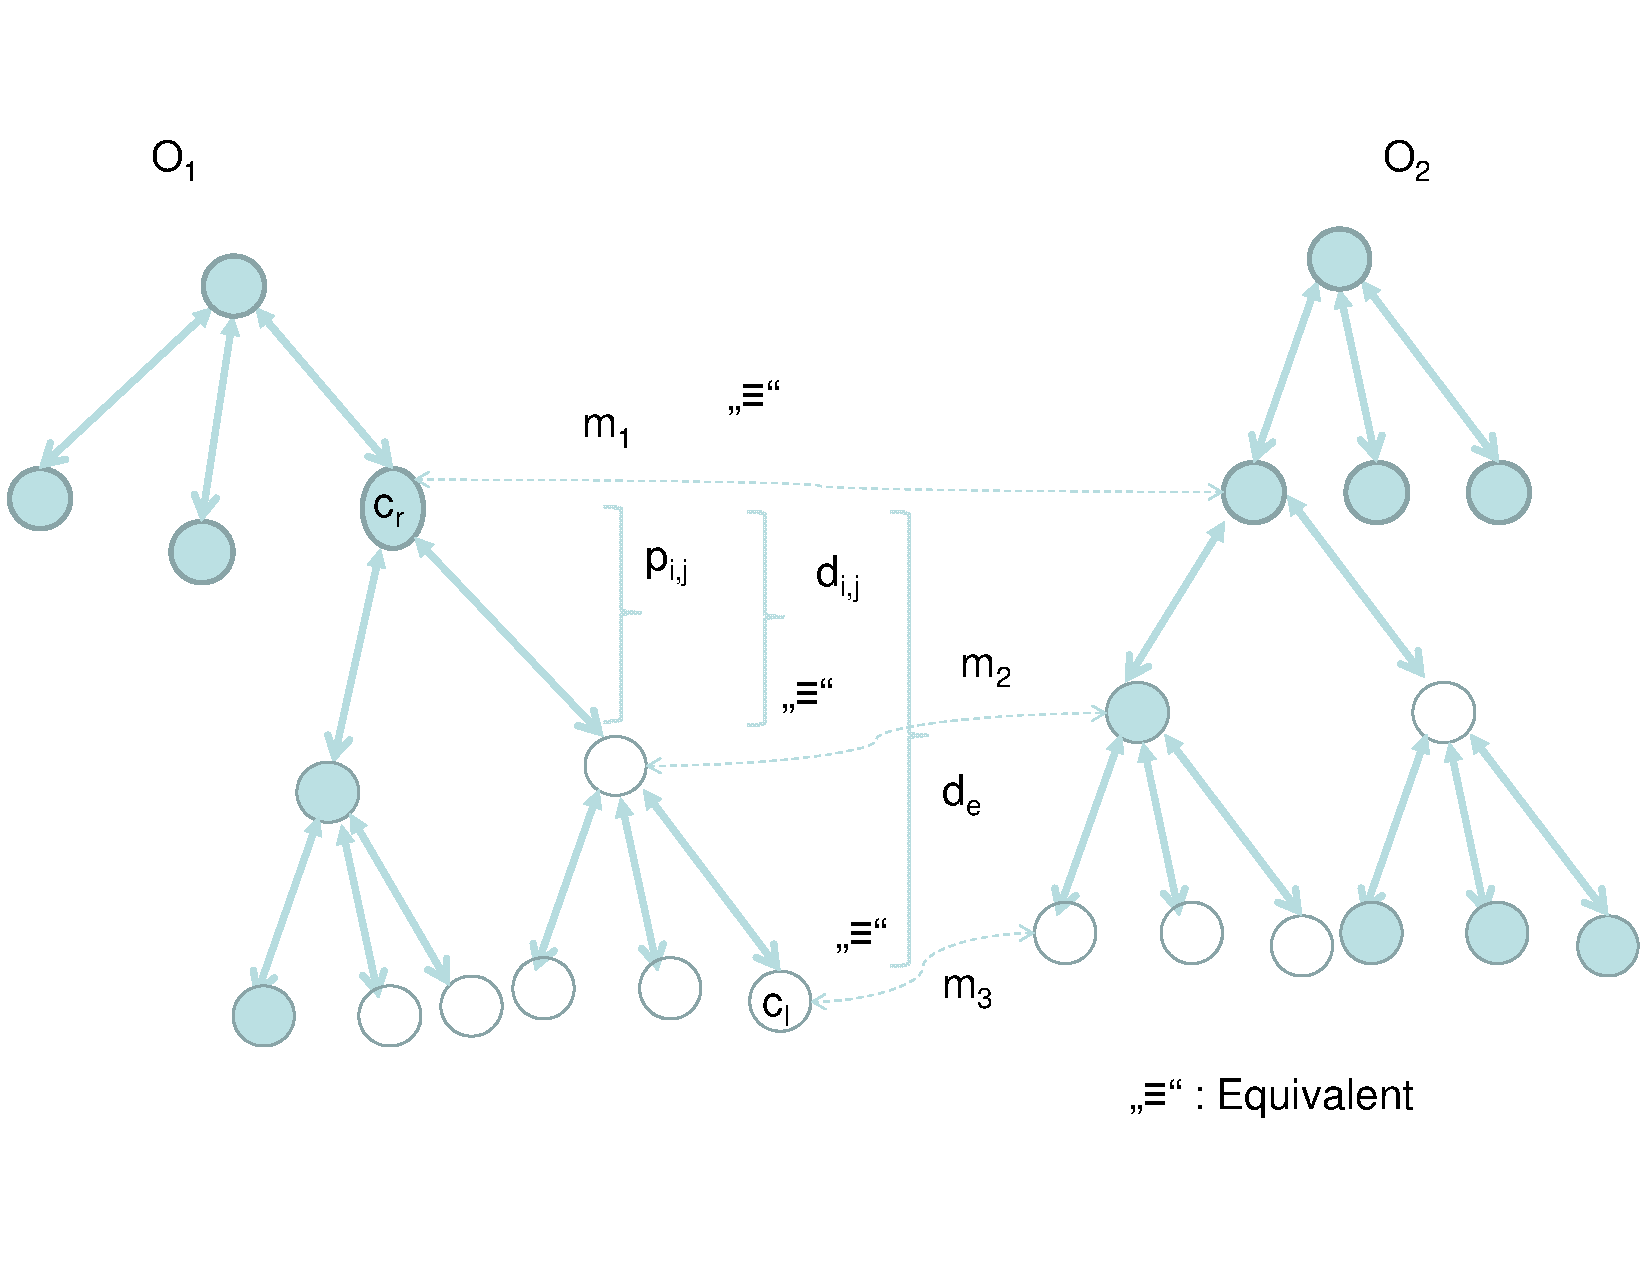
\includegraphics[scale=0.7, angle = 90]{figure-chapterIV/fig4-14.pdf}\\
	\caption{Hypermodule Structure}
	\label{figure4-14}
\end{center}
\end{figure}

Given that in the previous paragraphs we defined the required terminology, now it is possible to explain the procedure we intend to apply as follows. A first procedure, \texttt{preprocess\_repository}, is carried out on pairs of ontologies. This consists in  mapping both ontologies in order to find out similarity of concepts. Mappings that fill this requirement are stored in a \texttt{hypermatching\_record}. These mappings are not definitive and require a user check; this is done in \texttt{clean\_hypermatching\_record} procedure. This procedure consists in presenting the set of mappings obtained by the automatic procedure to an expert for validating them. Mappings considered as valid by experts are held in the data set, the others are deleted. \texttt{Hypermatching\_record} is then processed to generate hypermodules, first detecting modules. These are individual concepts that are hyper mapped, but they are not connected to any leaf concepts by means of subsumption arcs. If we find some of these, we store them in a \texttt{mono\_module\_record}, which maintains concepts and a reference to their mappings. 

If the hyper mapped evaluated concept is connected to leaf concepts, then the reference is instead stored in the \texttt{multi\_module\_record}. Afterwards, bounds are set for these modules, by identifying \texttt{hyper\_root} and {hyper\_leaf} concepts. With this information it is possible to group sets of concepts which are bounded by upper bounds and lower bounds. This is executed by the \texttt{set\_hypermodule} procedure, which consequently generates hypermodules as required. Fig.\ref{figure4-15} shows the pseudo code corresponding to hypermodule generation, starting with the consideration of a set of ontologies:

\begin{figure}
\vspace{-40}
\begin{center}
	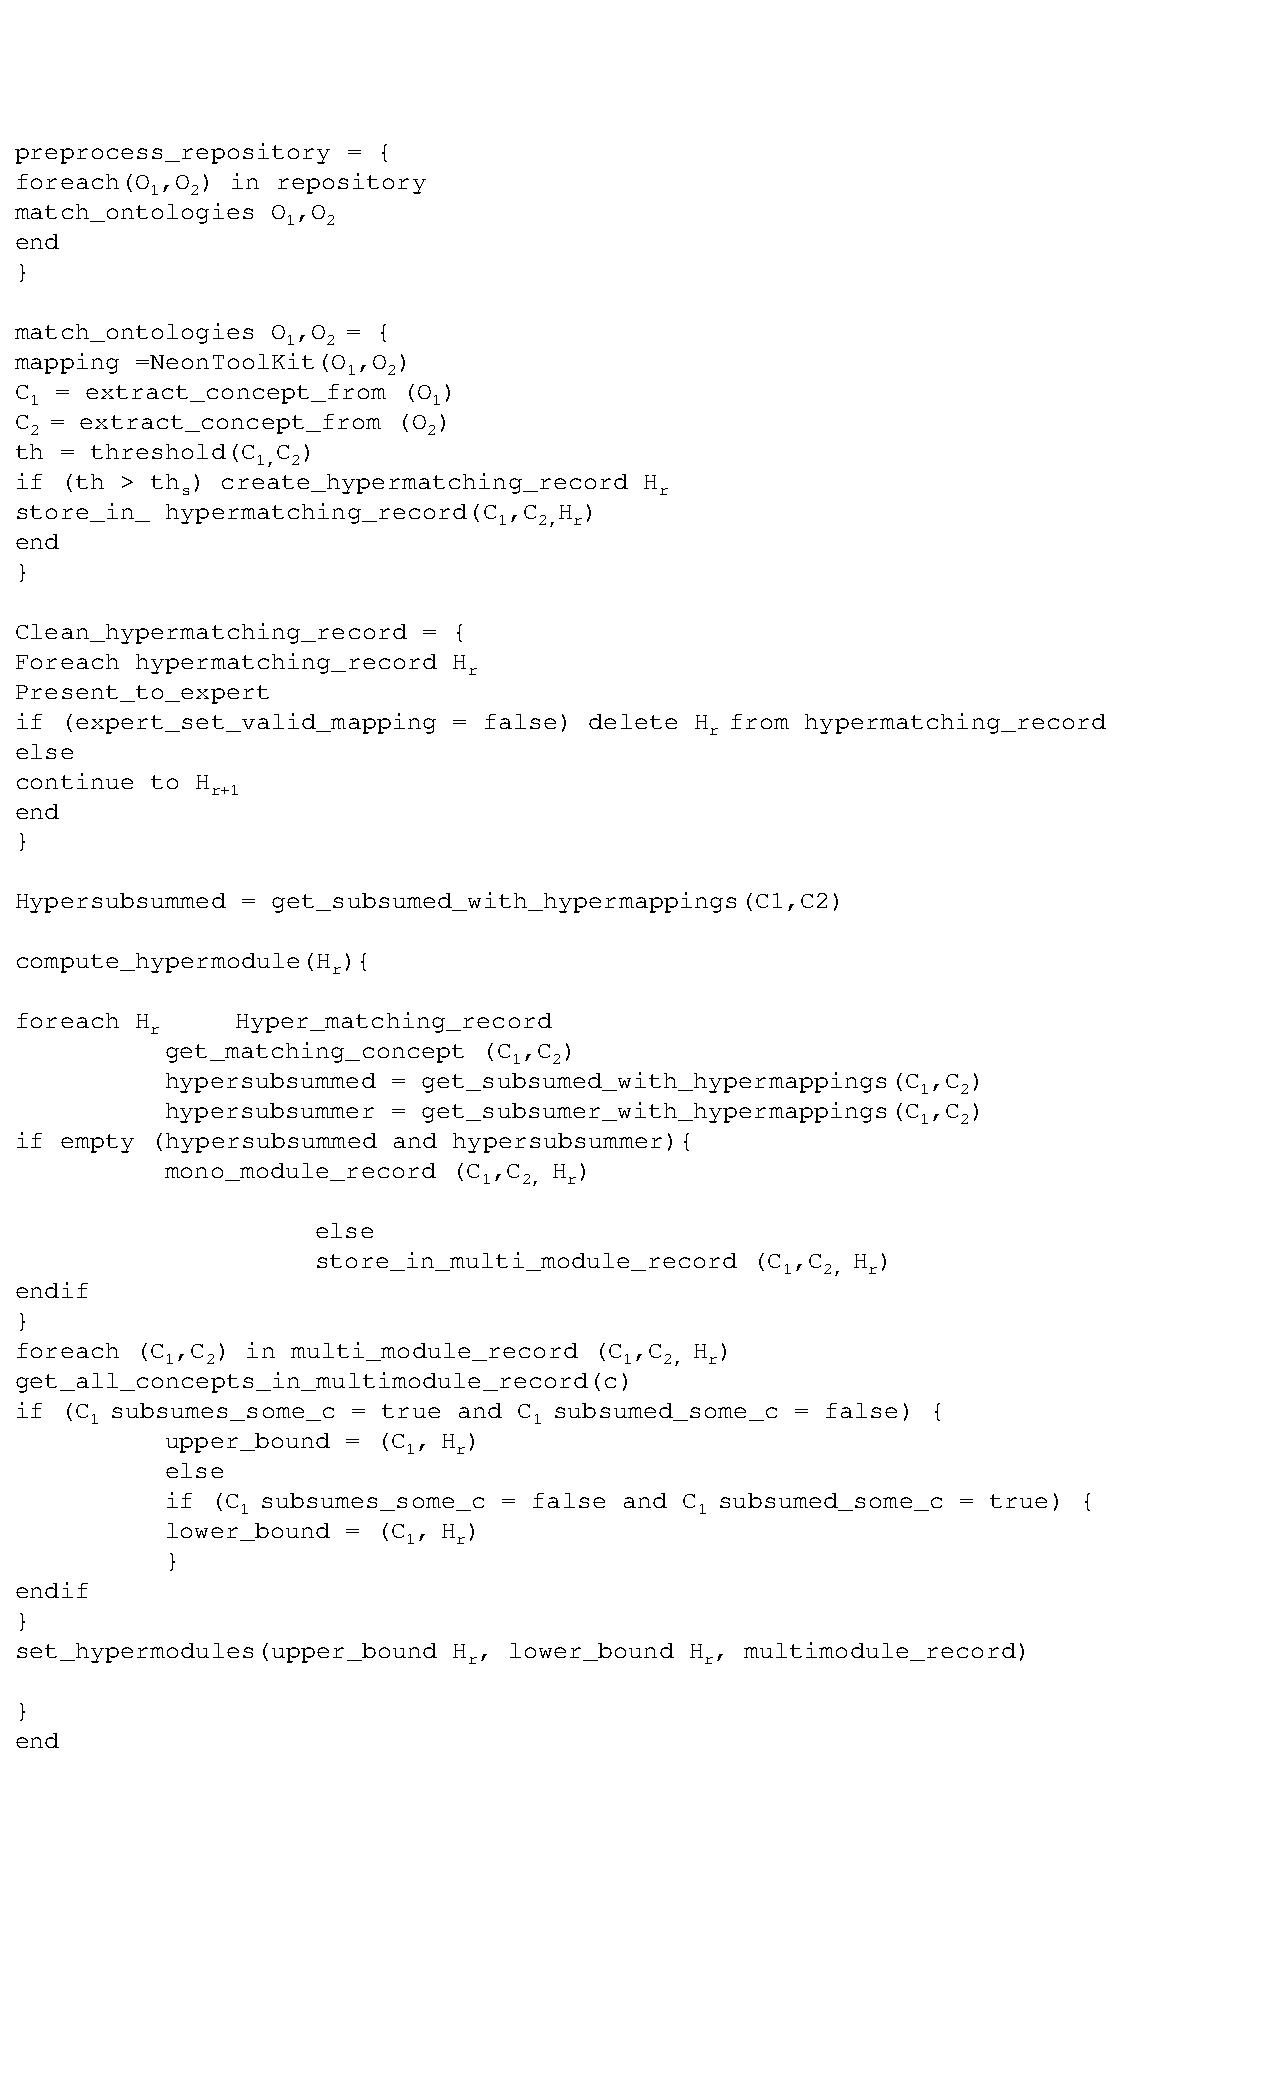
\includegraphics[scale=0.7]{figure-chapterIV/fig4-15.pdf}\\
	\vspace{-80}
	\caption{Pseudo Code for Hyper-modularization}
	
	\label{figure4-15}
\end{center}
\end{figure}




In the related literature we found a similar algorithm proposed by \cite{oliver_kutz_chinese_2010} to generate hyper modules from a multi-ontology environment. Our proposed algorithm presented in Fig.\ref{figure4-15} differs from this in that we include a validation procedure by an expert, the generation of two types of hyper modules, and that the creation of such modules is based in a closure procedure that includes the identification of root and leaf nodes or concepts. 

To complement the algorithm    introduced in Fig.\ref{figure4-15}, some metrics of hypermodule quality are included to provide the Ontological Engineer with tools to evaluate the resulting modules. 


\begin{itemize}
\item First, we present a metric based on a density criterion: in other words, the greater the number of concepts of the hyper module mapped to some concept in a target ontology, the better it is. The corresponding formula for calculating this is:
\end{itemize}	

\begin{equation}\label{eq.4.7}
$$	
MQ = \dfrac{\sum_{j=1}^{P_{i,j} }N_{C_{h} \in C_{u}}}{\sum_{k=1}^{P_{i,j}}N_{C_{ \in C_{u}}}}$
$$
\end{equation}


Where MQ corresponds to the quality of the module under evaluation, $P_{i,j}$  corresponds to a given subsumption arc where a hyper mapped   concept of a hyper module is present; furthermore    $N_{C\in C_{u}}$corresponds to the number of all concepts that are subsumed by $C_{u}$, and $N_{Ch \in Cu}$ corresponds to the number of those concepts that are equally subsumed by $C_{u}$, but have hypermappings to some other ontology. The formula returns a value between 0 and 1. The higher the value, the better the quality \textbf{why}. 

\begin{itemize}

\item	Secondly, we also want to know the numerical relation between a concept in a section of the hyper mapped network and the same concept in the total network. The greater presence of the given concept in both cases, the better it is. For this metric we define the following sets:

\begin{itemize}
	\item 	For each ontology $O_{h}$, the set of nodes $C_{hs}$ \in $O_{h}$ which are subsumed by a mapped concept.
	
	\item 	$N_{O_{d}}$  corresponds to the number of all  ontologies $O_{d}$ of the domain under study.
	
	\item 	$N_{O_{b}}$  corresponds to the number of   ontologies of the domain under study which have a mapped concept. $N_{O_{b}} \leq N_{O_{d}} $.
	
\end{itemize}



\end{itemize}


After defining the sets, we can then define the following metrics:

\begin{itemize}
\item Bounded Strength:
\begin{equation}\label{eq.4.8}
	BS = \dfrac{N_{C_{hs}\in O_{h}}}{N_{O_{d}}}
\end{equation}

Where $N_{C_{hs}\in O_{h}}$  corresponds to the number of times that a concept of a hyper module appears in the network of ontologies and  ${N_{O_{d}}}$ was defined above.  


\item Domain Strength

\begin{equation}\label{eq.4.9}
	DS = \dfrac{N_{C_{hs}\in O_{h}}}{N_{O_{b}}}
\end{equation}


Where $N_{C_{hs}\in O_{h}}$ and ${N_{O_{b}}}$ were explained for the previous metric. 

\end{itemize}



After defining the corresponding metrics for quantifying the quality of the hyper modules to be extracted from the network of ontologies shown in Fig. \ref{figure4-11}, we proceeded to execute the pseudo-code introduced in Fig. \ref{figure4-15} in order to obtain hyper modules, if any. Within this specific procedure we continue with our proposed methodology, specifically in the \texttt{Hyper-Rel} and \texttt{Modularity} activities.  \textbf{where?}

By the subroutine \texttt{compute-hyper module} it is possible to obtain two groups of hyper modules (\texttt{mono-modules} and \texttt{multi-modules}) from the network of ontologies shown in Fig. \ref{figure4-11} above.  Table \ref{table4.6} lists a first set of mono-modules, concepts which are mapped according to the proposed algorithm with the particularity that they do not have leaf concepts, so we call them   mono-modules or individual mappings. Nevertheless, mono-modules should not be discarded, because the presence of these concepts in a network of ontologies can contribute to interoperability. 

\begin{table}[tp]%

\caption{List of Monomodules}
\label{table4.6}\centering
\begin{tabular}{ p{4cm}}\toprule
	
	\textbf{Monomodules} \\\toprule
	Event\\\toprule
	Material\\\toprule
	Set\\\toprule
	Organization\\\toprule
	Person\\\toprule
	
\end{tabular}

\end{table}


As we indicated above, with the implementation of our algorithm in the network of ontologies presented in Fig. \ref{figure4-11} it was also possible to find a group of six hyper-modules of multi-module type. Every multi-module, as we defined them within the subroutine \texttt{compute-hypermodules}, contains several concepts subsumed by a root concept which in turn is connected to another concept in another ontology through mapping. These modules were named \texttt{Unit, Product, Process, Features, Resources} and \texttt{Geometry}. Regarding the specific concepts, it is necessary to remember the list of concepts mentioned in Subsection \ref{subsection2.2.1} proposed by \cite{martin_design_2003} and \cite{lastra_ontologies_2009} as significant for the manufacturing domain. Those terms are \texttt{Product, Process, Resource} and \texttt{Equipment}. Moreover, we are including the root concepts \texttt{Unit, Features, Geometry} and the concepts \texttt{event, material, set, organization} and \texttt{person} (\texttt{mono-modules}). With this information we proceeded to present every resulting hyper module of multi-module type, at first for every-module evaluating graphics is presented, and then an ontological view of the module is shown, this view was obtain after editing the hierarchical view of the hyper module in an ontology editor, Protégé for this case. After describing every hyper module, they will be included in a single view that integrates the hyper modules of the hyper ontology with the network of ontologies.

\subsubsection{Hyper module of Unit}\label{subsubsection4.2.5.1}

In Subsection \ref{subsection4.2.4} we introduced Table \ref{table4.5} to present the most frequent terms found in the network of ontologies shown in Fig. \ref{figure4-10}. With the application of our proposed algorithm, the concept \texttt{Unit} appears again as a part of a hyper module of multi module type. This concept is integrated with the concepts \texttt{BaseUnit}, \texttt{Mega}, \texttt{micro}, \texttt{meter} and \texttt{degree Celsius}. It is necessary to mention the relevance of these terms for Science and Engineering,   given that metrology, as the science of measurement, takes part in those fields. Nevertheless, besides the importance of the term   \texttt{Unit} for manufacturing, it  does not appear in every ontology of the network; moreover the other terms that form part of this hyper module appears in only 2 of those ontologies.   

In Fig. \ref{figure4-16} we show the results obtained calculating the values of BS and DS  of the concept \texttt{Unit}   and some of its subsumed terms among ontologies included in network  shown in Fig. \ref{figure4-11}. There, the concepts present in this multi-module are evaluated in two steps: first an evaluation of the ontologies that contain the concept \texttt{Unit} and, second, around every term subsumed by \texttt{Unit}. Most of the terms presented there have a bounded strength (BS) of 0.4 and a domain strength (DS) of 0.26. This result means that, although the BS is closer to 50\%, when measuring the domain under study, the average DS indicates a weakness more than a strength on the terms related to \texttt{Unit}. Going into details, the term \texttt{Unit} is presented in 5 of 8 ontologies of the network, while the other terms are present only in 2 of 8. 






\begin{figure}
\begin{center}
	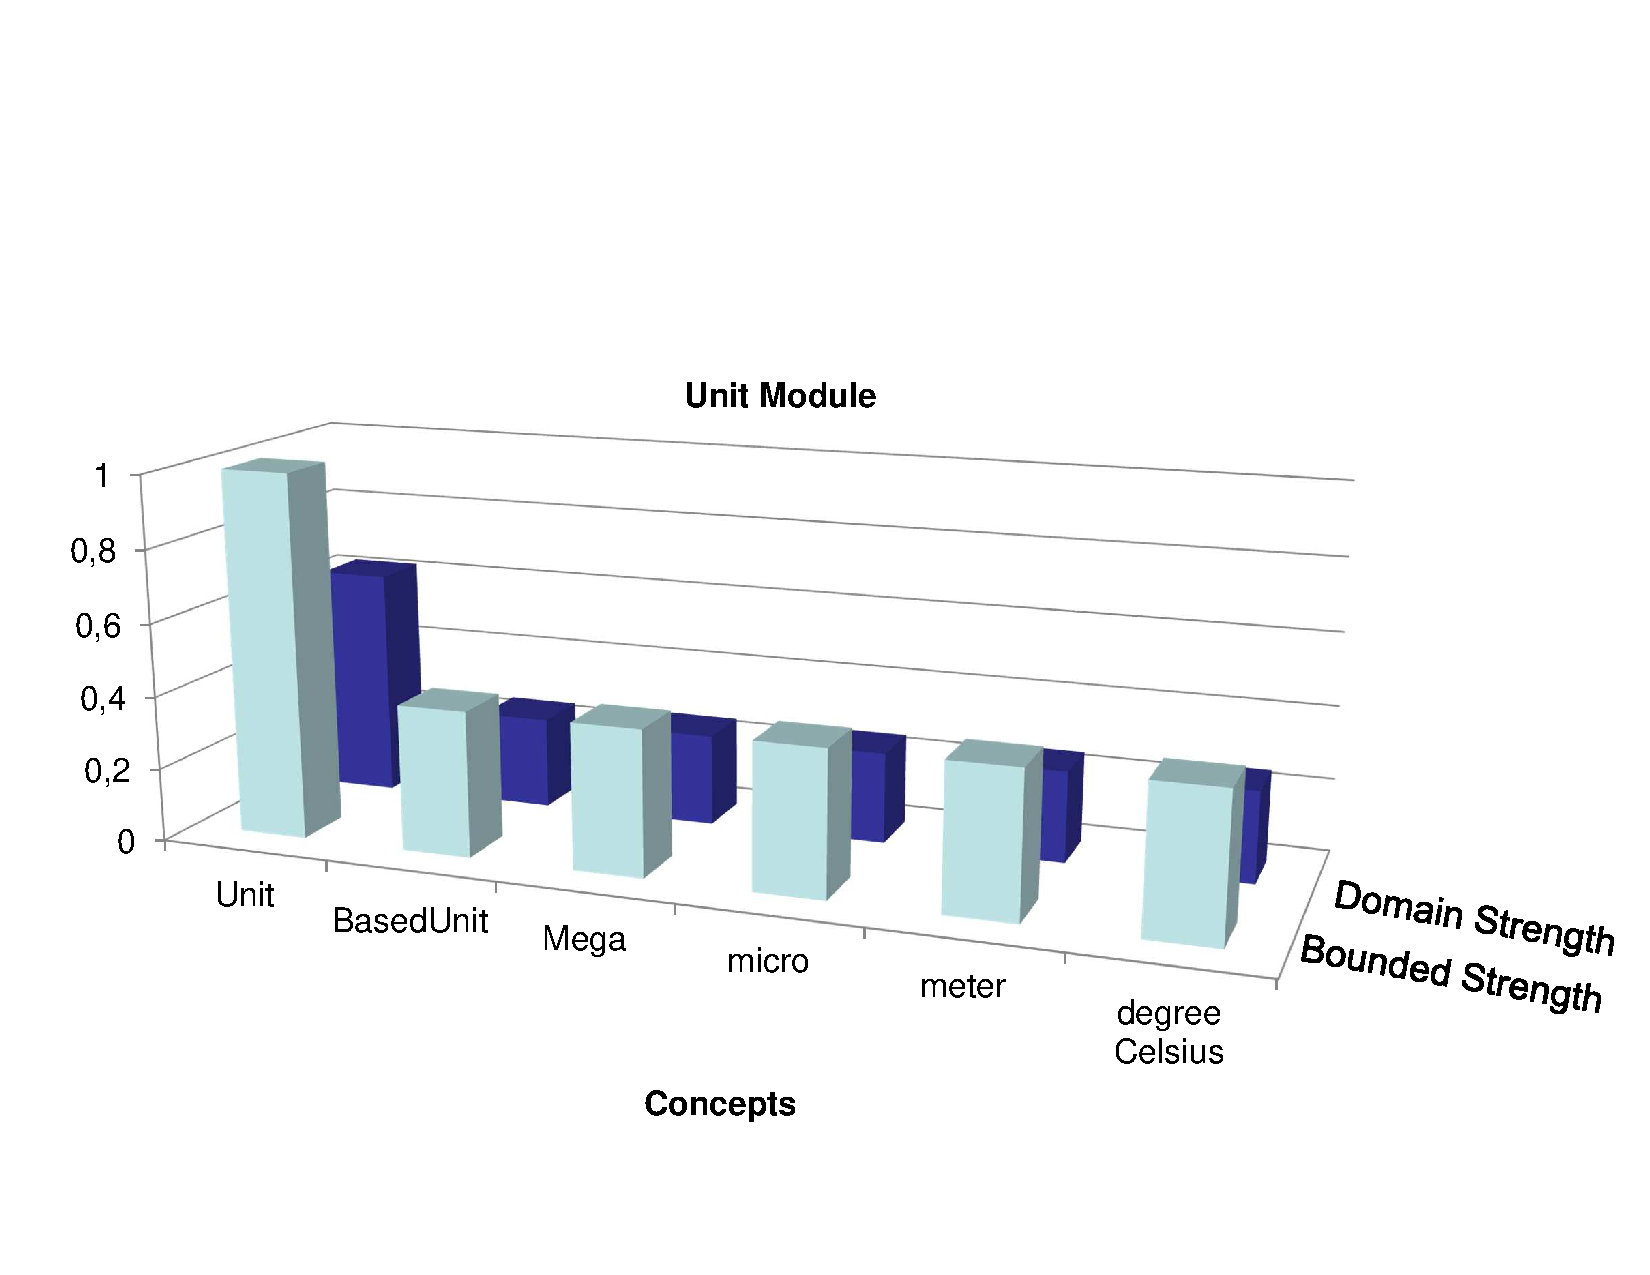
\includegraphics[scale=0.5]{figure-chapterIV/fig4-16.pdf}\\
	\caption{Strength of Concepts Bounded by Unit}
	\label{figure4-16}
\end{center}
\end{figure}

\begin{figure}
\begin{center}
	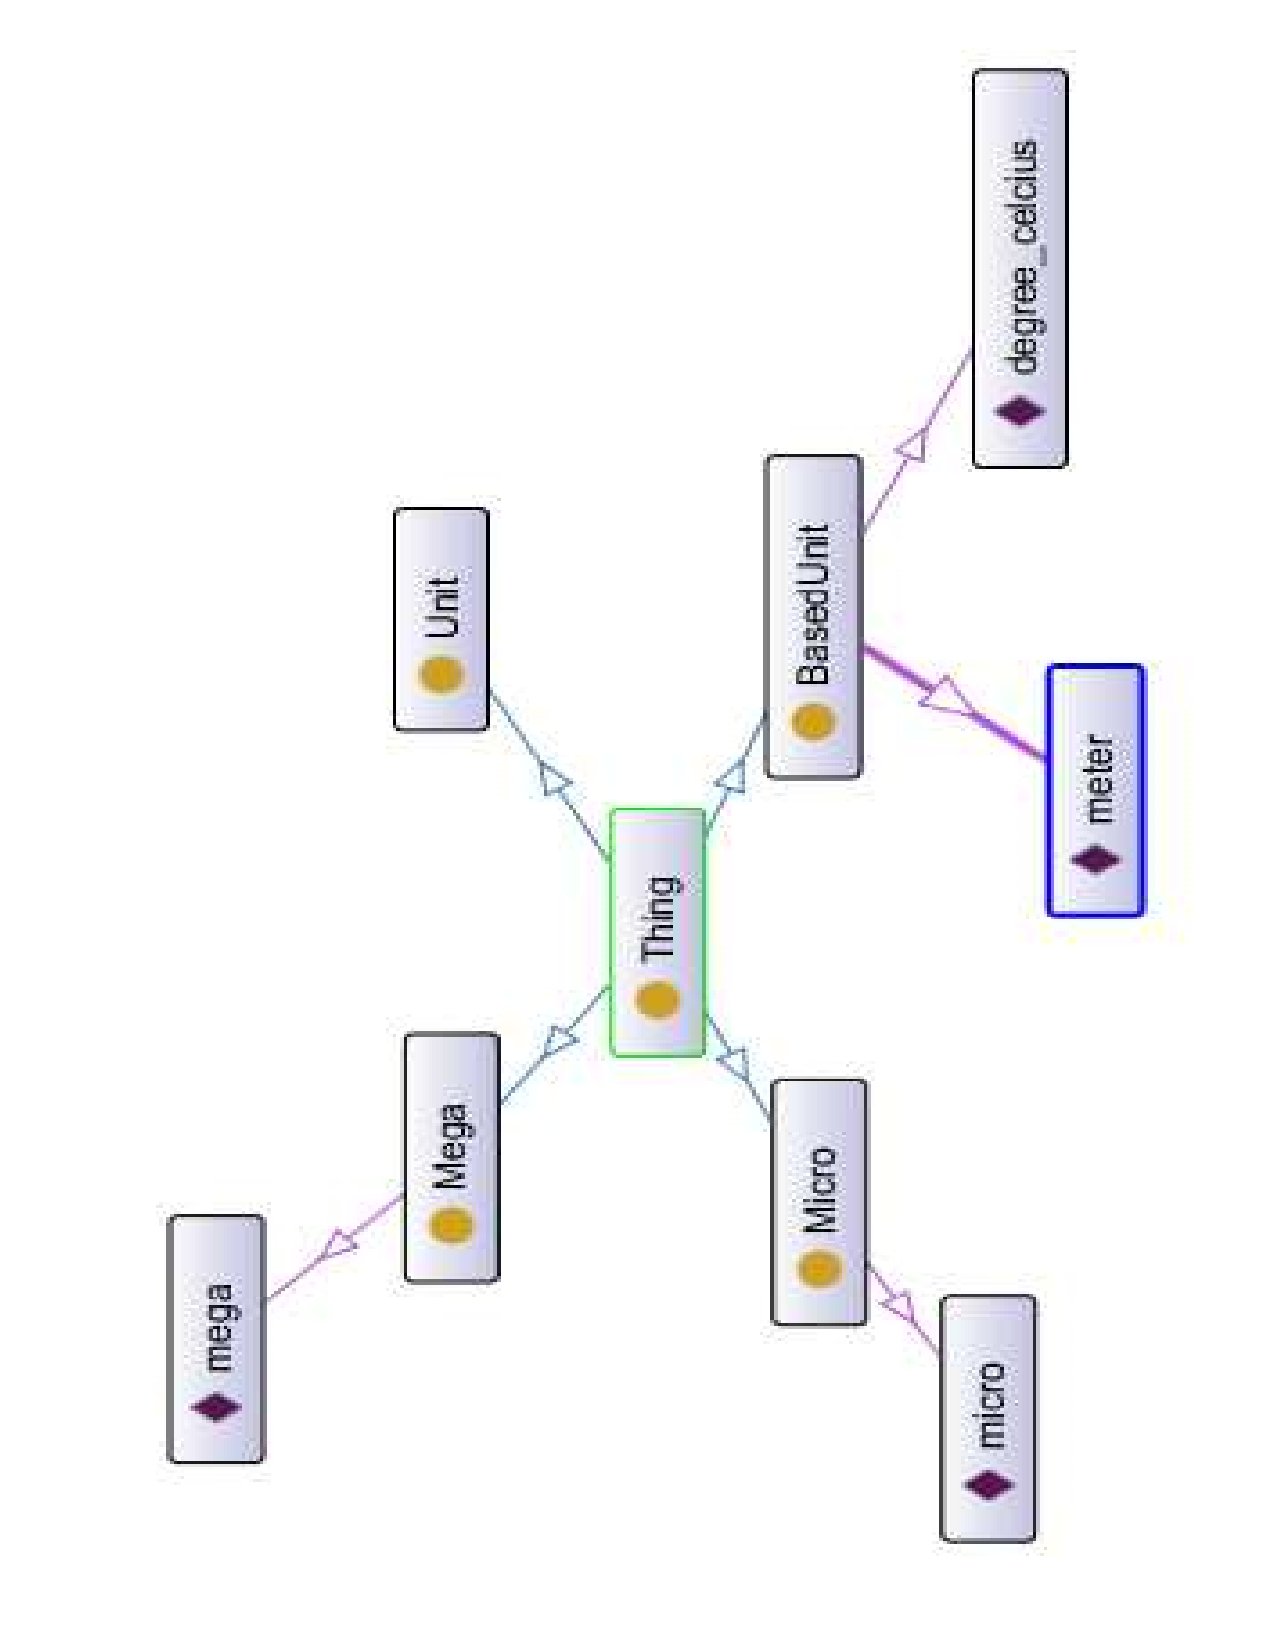
\includegraphics[scale=0.5, angle =270]{figure-chapterIV/fig4-17.pdf}\\
	\caption{Partial Hyperontology for the term \texttt{Unit} graphed with Protégé}
	\label{figure4-17}
\end{center}
\end{figure}


Fig. \ref{figure4-17} shows the concepts and instances that appear mentioned in Fig. \ref{figure4-16}. This set of concepts was obtained as a partial result of executing the \texttt{compute\_hypermodule} routine which is part of our algorithm. This figure shows the result as an ontology. 

\subsubsection{Hyper module of Product}\label{subsubsection4.2.5.2}

Similarly, and following the procedure described above, the Hyper module \texttt{Product} was obtained. This hyper module is integrated   by the terms \texttt{Product, Part} and \texttt{Assembly}. It is worth noting the relevance of these terms in Semantic Manufacturing because,   on the one hand the Product can be considered the center of this conceptualization, and products many times are integrated by some type of parts, generating an assembly. On the other hand the presence of the concepts \texttt{Part} and \texttt{Assembly} in this hyper module indicates the existence of a relation that comprises the product, and this type of relation is known as parthood relations. In Section \ref{subsection2.2.3}, parthood relations were introduced as a shortcoming of   OWL, in cases where such an ontology language is used. Later, as part of our methodology, when Axiomatiozation and Hetereogeneity activities take place, the parthood relations issued by OWL, will be taken up and discussed. Below we present the analysis related to this hyper module. 


\begin{figure}
\begin{center}
	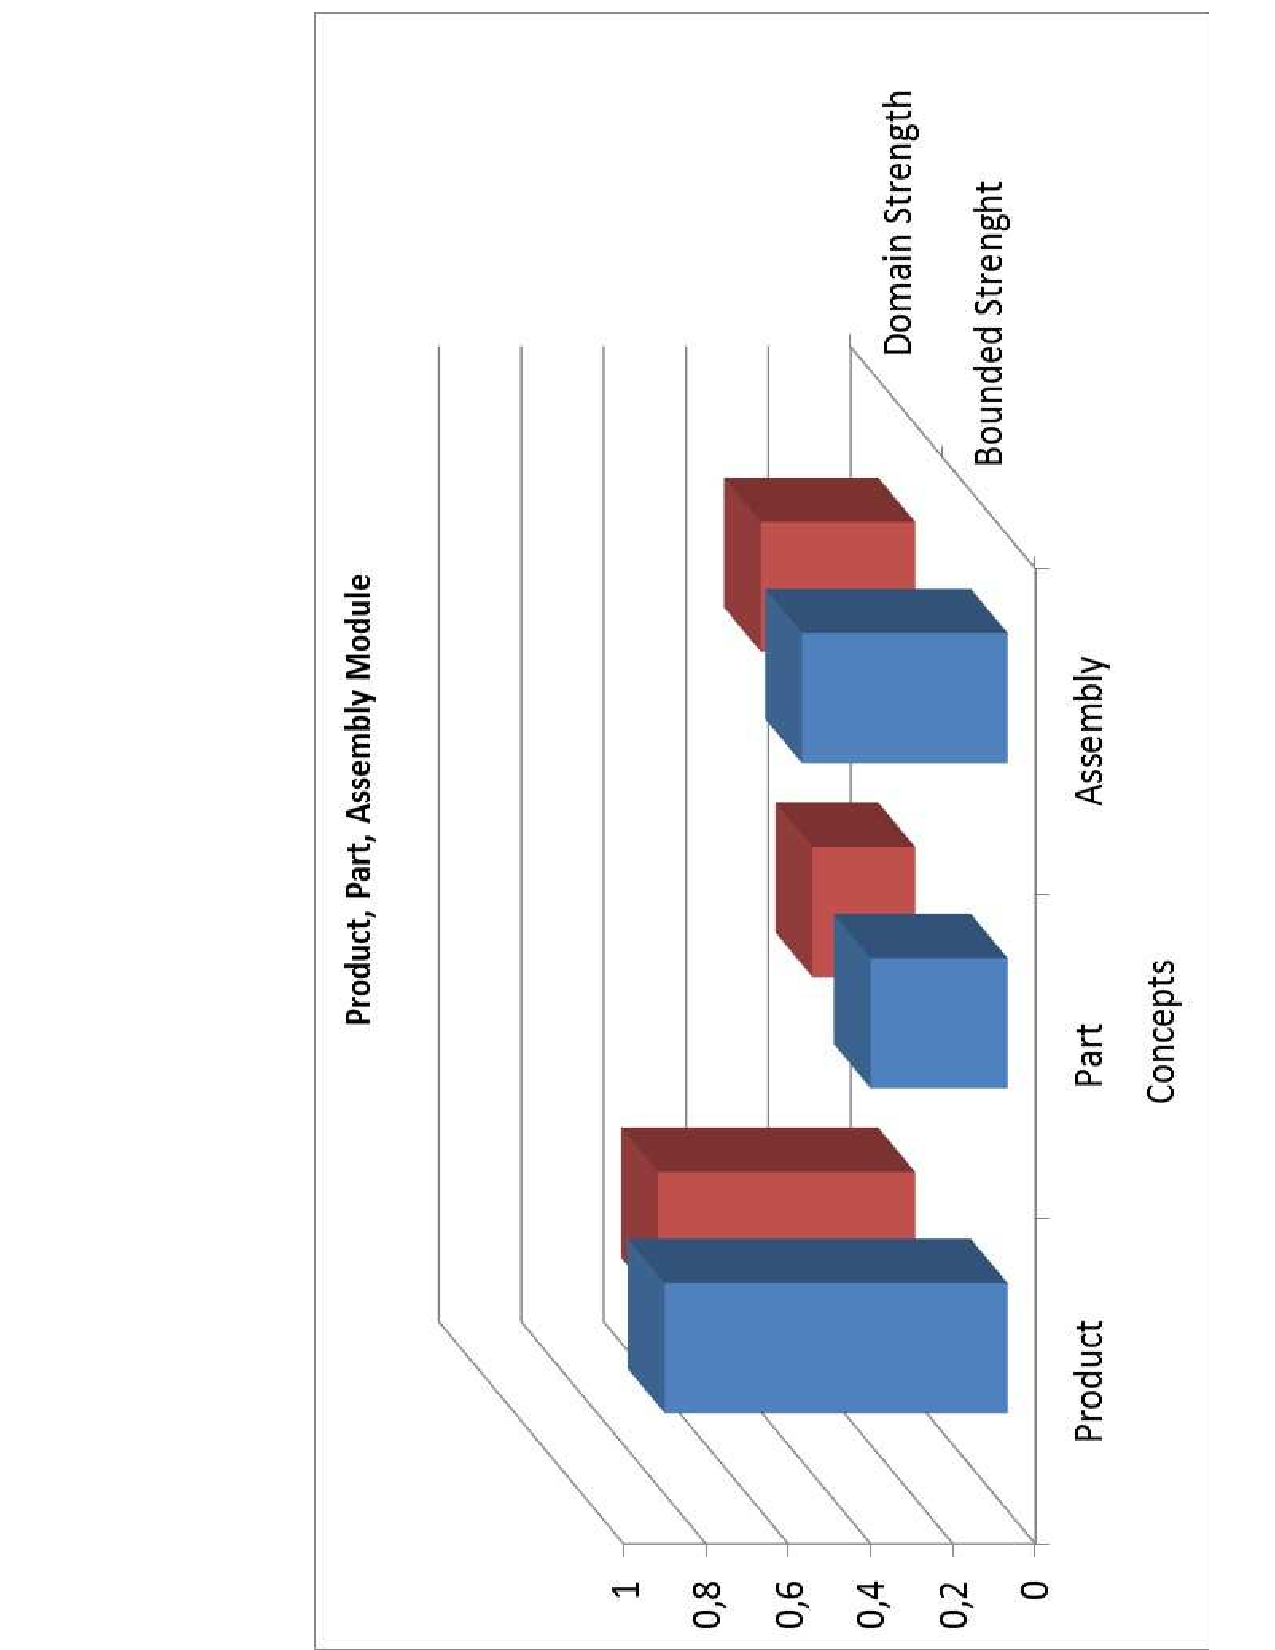
\includegraphics[scale=0.5, angle=-90]{figure-chapterIV/fig4-18.pdf}\\
	\caption{Product Hyper Module}
	\label{figure4-18}
\end{center}
\end{figure}

\begin{figure}
\begin{center}
	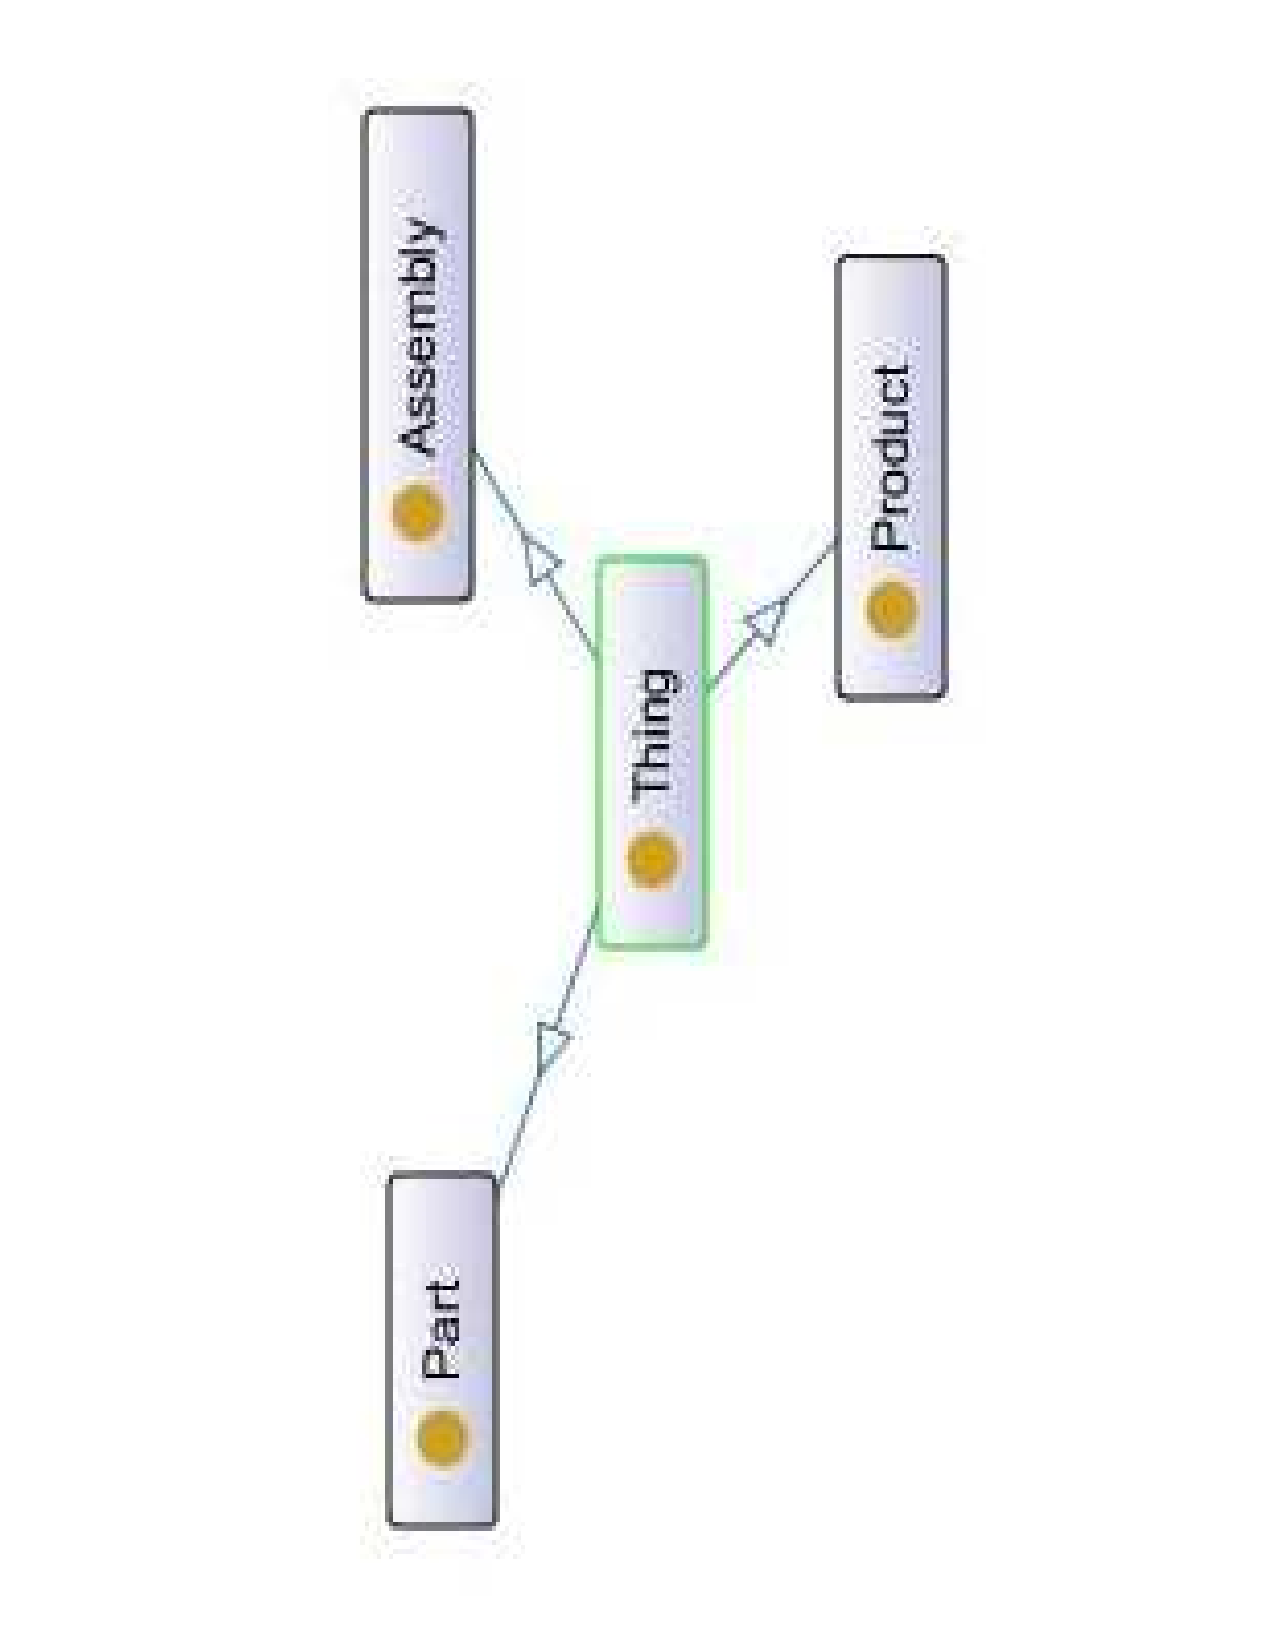
\includegraphics[scale=0.5, angle=270]{figure-chapterIV/fig4-19}\\
	\vspace{-20}
	\caption{Members of the Hypermodule Product}
	\label{figure4-19}
\end{center}
\end{figure}


Fig. \ref{figure4-18} shows the results of the statistical analysis we performed, which is the term \texttt{Product} has a BS of 0.83, followed by \texttt{Assembly} with a BS of 0.5; and the term \texttt{Part} with a BS of 0.33 Moreover \texttt{Product} has a DS of 0.625 followed by \texttt{Assembly} and \texttt{Part} with a DS of 0.375 and 0.25 respectively. In the case of the term \texttt{Part}, and following a criterion similar to the one used for the hyper module \texttt{Unit}, we can state that there is a weakness in it, which means there is a low likelihood of achieving interoperability through it.  After analyzing  this hyper module according to the proposed BS and DS metrics, we proceed to represent it as an ontology in Fig. \ref{figure4-19}. This figure corresponds to a simplified view given that the corresponding ontologies, and other hyper-modules have to be integrated in a complete view, present in the hyper ontology as integrated by hyper modules in an ontologies network. 


\subsubsection{Hyper-module of the Process}\label{subsubsection4.2.5.3}

Following the statistical   analysis of results, Fig. \ref{figure4-20} introduced the hyper module of \texttt{Process}. \texttt{Process} and \texttt{Operation} are meaningful concepts for the manufacturing domain. In this vein, the concept \texttt{Process} has been mostly adopted to define ontologies related to this terminology. Nevertheless, from the graphic it can be concluded that in this network the concept \texttt{Operation} is found with more strength   (BS: 0.6) than the concept \texttt{Process} (BS: 0.4). Other terms found in this hypermodule were \texttt{Change}, related to \texttt{Process} and \texttt{Operation}, and the terms \texttt{Cutting, Drilling, Milling} and \texttt{Addition}. 

The last four terms mentioned above are closely related (\texttt{Cutting}, \texttt{Drilling}, \texttt{Milling} and \texttt{Addition}), given that   the three terms correspond to a manufacturing application domain named machining, and all of them belong to MASON. We go into details of these results because the authors of MASON declared it is an Upper Level Ontology. These concepts have a low BS and DS (0.2 and 0.125 for each respectively) which makes them highly usable, but less reusable because of their specificity. This result is not necessarily related to quality, because the effectivity of this ontology will depend more on the skills of the ontologist than the ontology itself. But, the resulting values of BS and DS of those MASON concepts serves  to categorize MASON as an Application Domain Ontology according to the categorization  shown in Fig. \ref{figure2-1} (Chapter \ref{chapter2}). This is not an isolated result. In Section \ref{subsection2.4.1} we  mentioned the research of other authors who have made similar remarks about their work, but with the implemented metrics,  procedures followed, and results obtained, the classification made by these authors  on  ontologies as ULO´s can be questioned. 


\begin{figure}
\begin{center}
	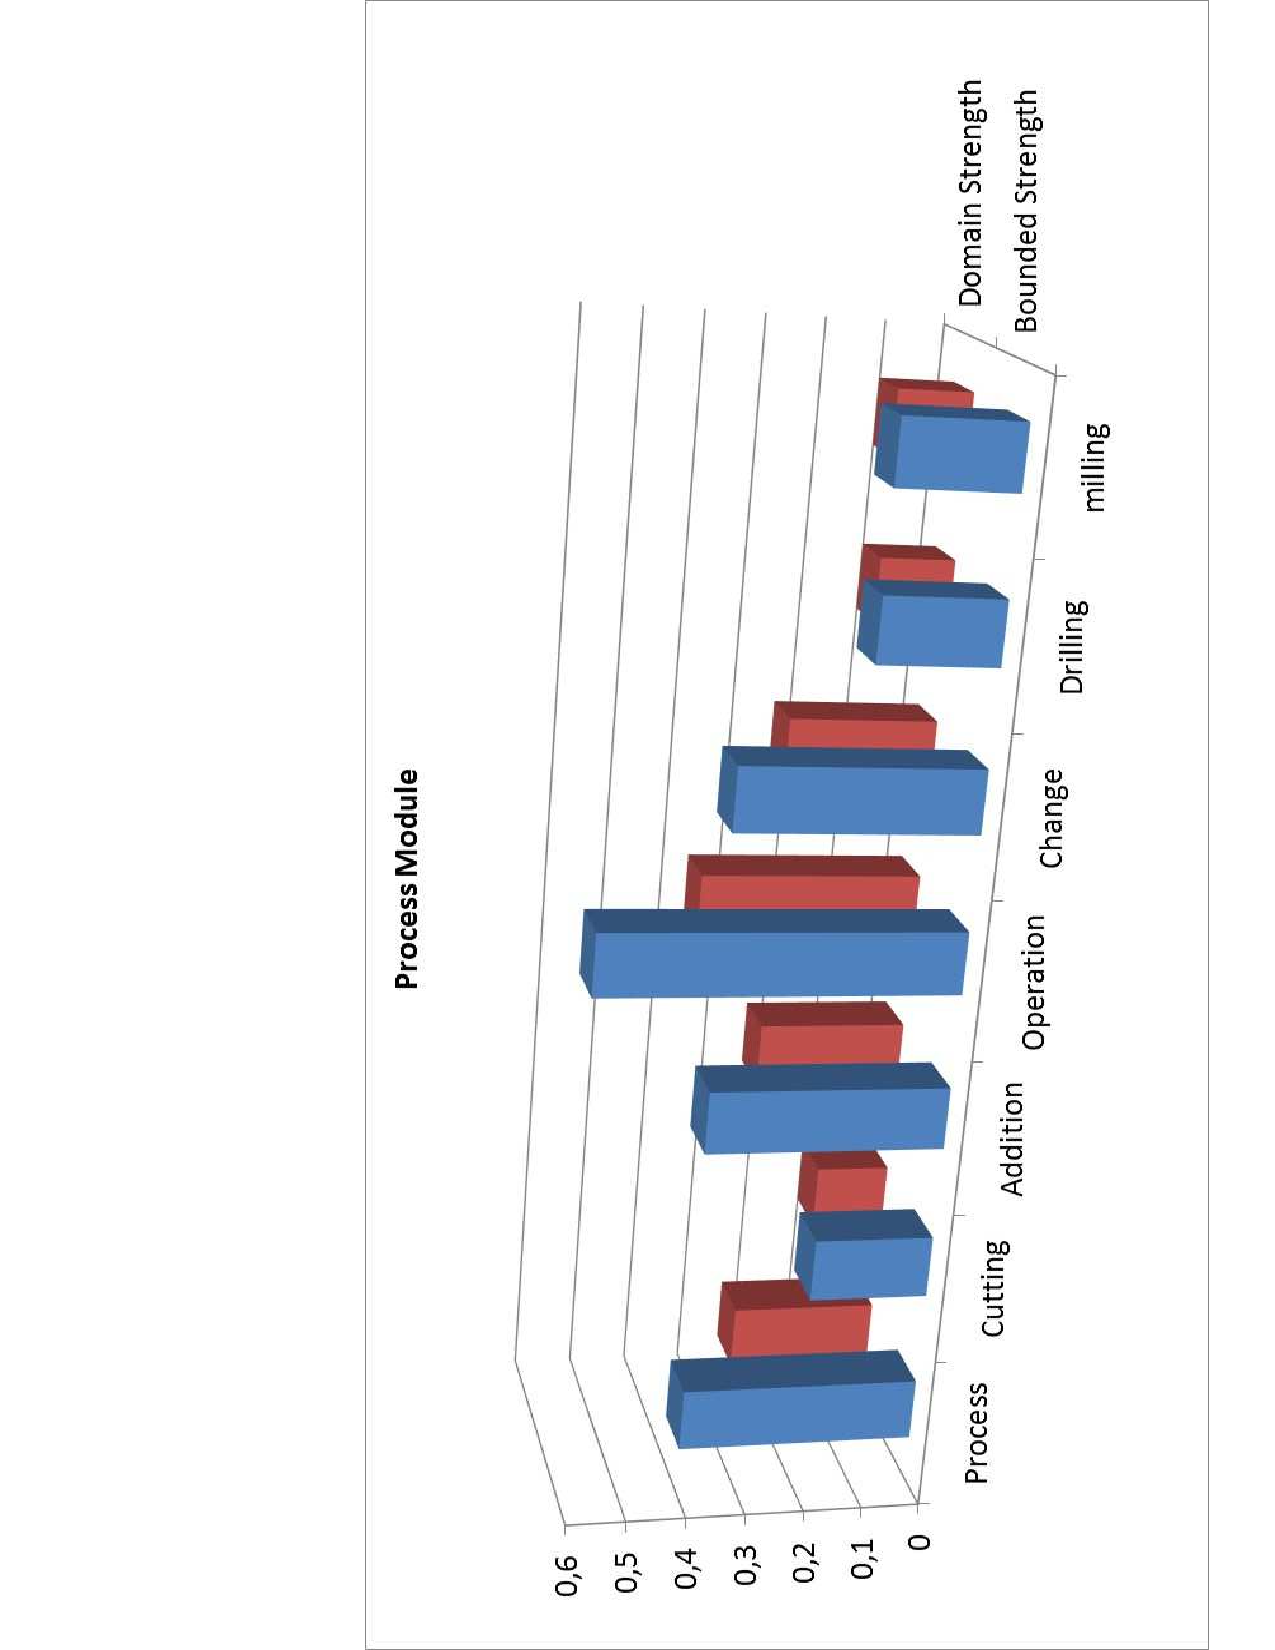
\includegraphics[scale=0.5, angle=-90]{figure-chapterIV/fig4-20}\\
	\caption{Hyper Module Process}
	\label{figure4-20}
\end{center}
\end{figure}

\begin{figure}
\begin{center}
	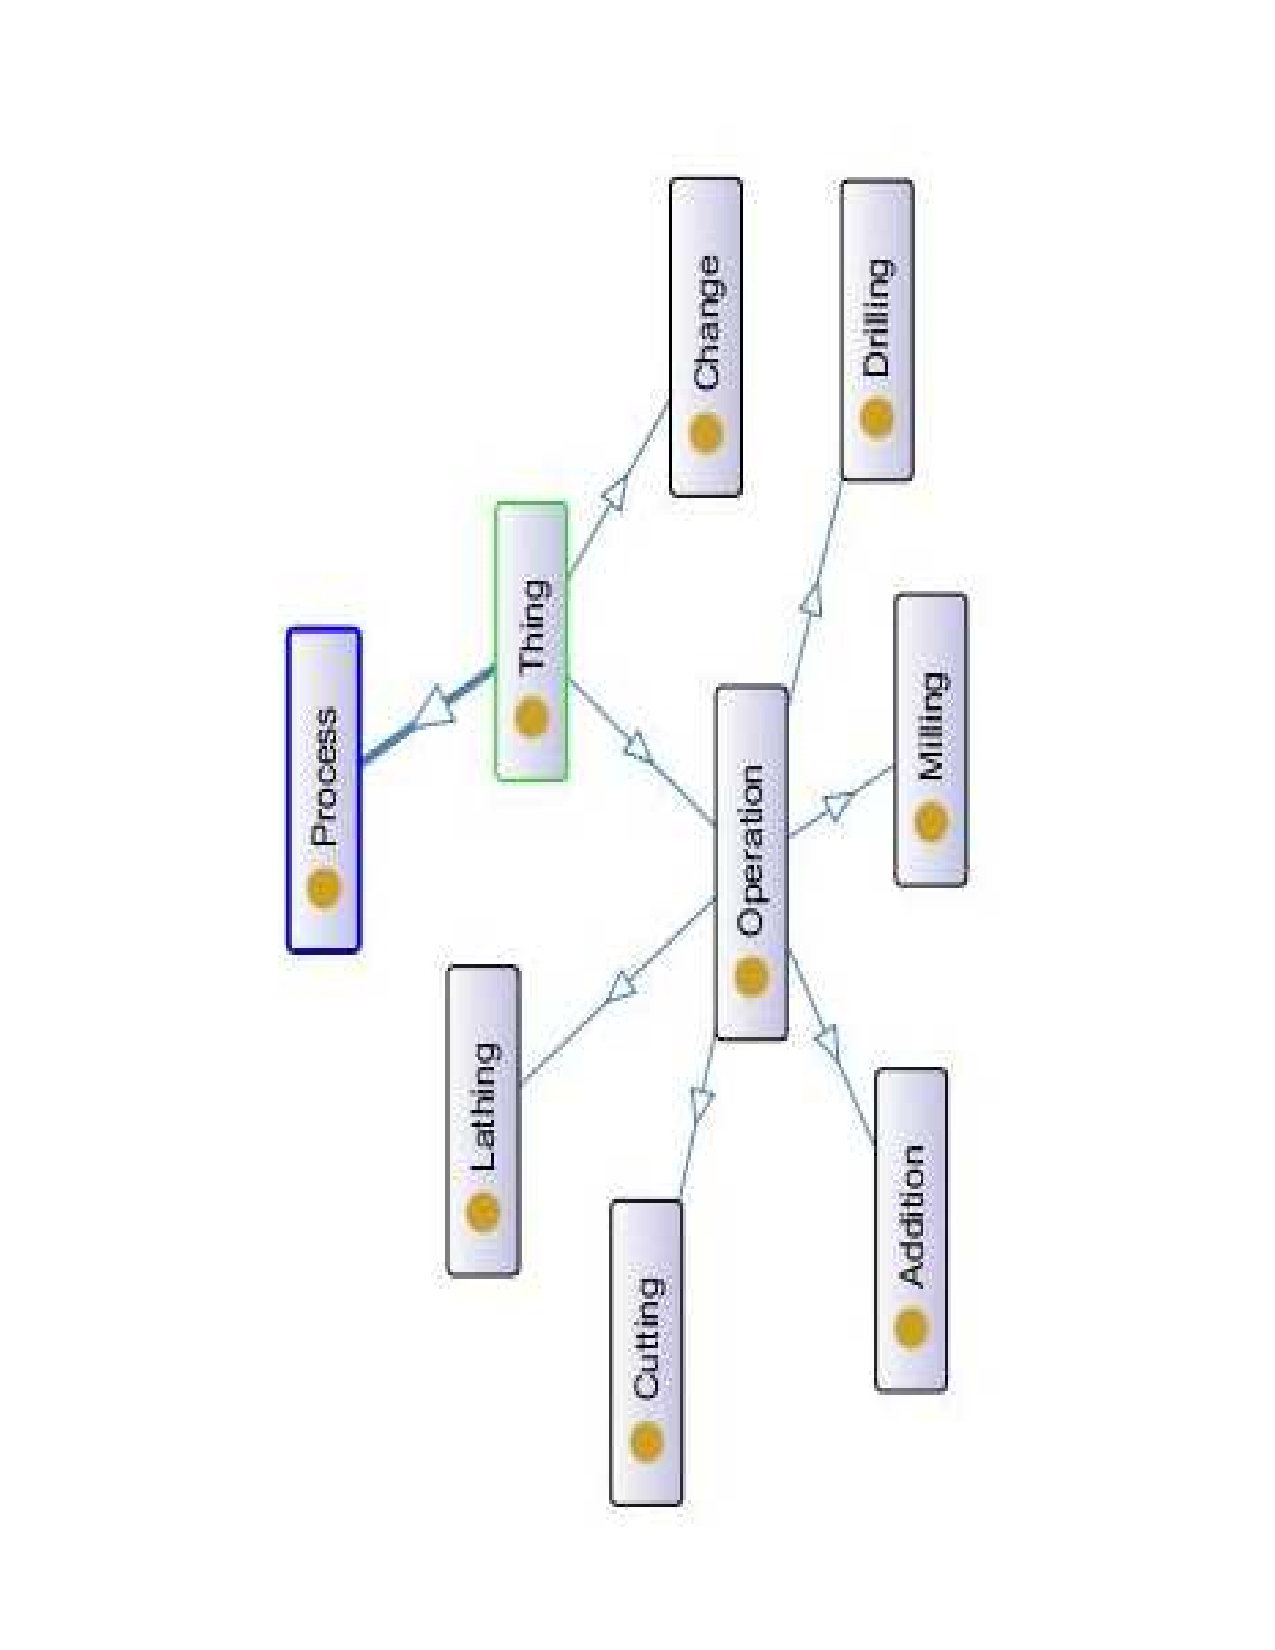
\includegraphics[scale=0.5, angle=270]{figure-chapterIV/fig4-21}\\
	\vspace{-40}
	\caption{Hyperontology of Process}
	
	\label{figure4-21}
\end{center}
\end{figure}

In Fig. \ref{figure4-21} we introduce an ontological view of the Hyperontology of the \texttt{Process} as resulting from Fig. \ref{figure4-21}. The concept \texttt{Operation} was used as root concept for specific operations due to its higher DS (0.375), while \texttt{Process} and \texttt{Change} remained  at the same \texttt{Operation} level. \textbf{meaning}

\subsubsection{Hyper module of Features}\label{subsubsection4.2.5.4}


Continuing with our hypermodule extraction, we processed a hyper module containing some features commonly found in mechanization processes. We named this the hyper module of features. Some of the concepts contained by this module are \texttt{Circular\_Pattern}, \texttt{Threat}, \texttt{Slot}, \texttt{Pocket}, and \texttt{Chamfer}. Most of the terms were found in MASON and Onto STEP, which will allow information exchange among both ontologies. It is necessary to highlight that the features mentioned below are common in mechanization processes, but they are not the only ones and they were also not found in the other 6 ontologies \textbf{... here}. For instance, PRONTO was proposed to represent products and their features, however no hyper-mapping was found in the network, because   they referred to different Application Domains: MASON corresponds to machining processes, and PRONTO to breaking up or separating processes.


\begin{figure}
\begin{center}
	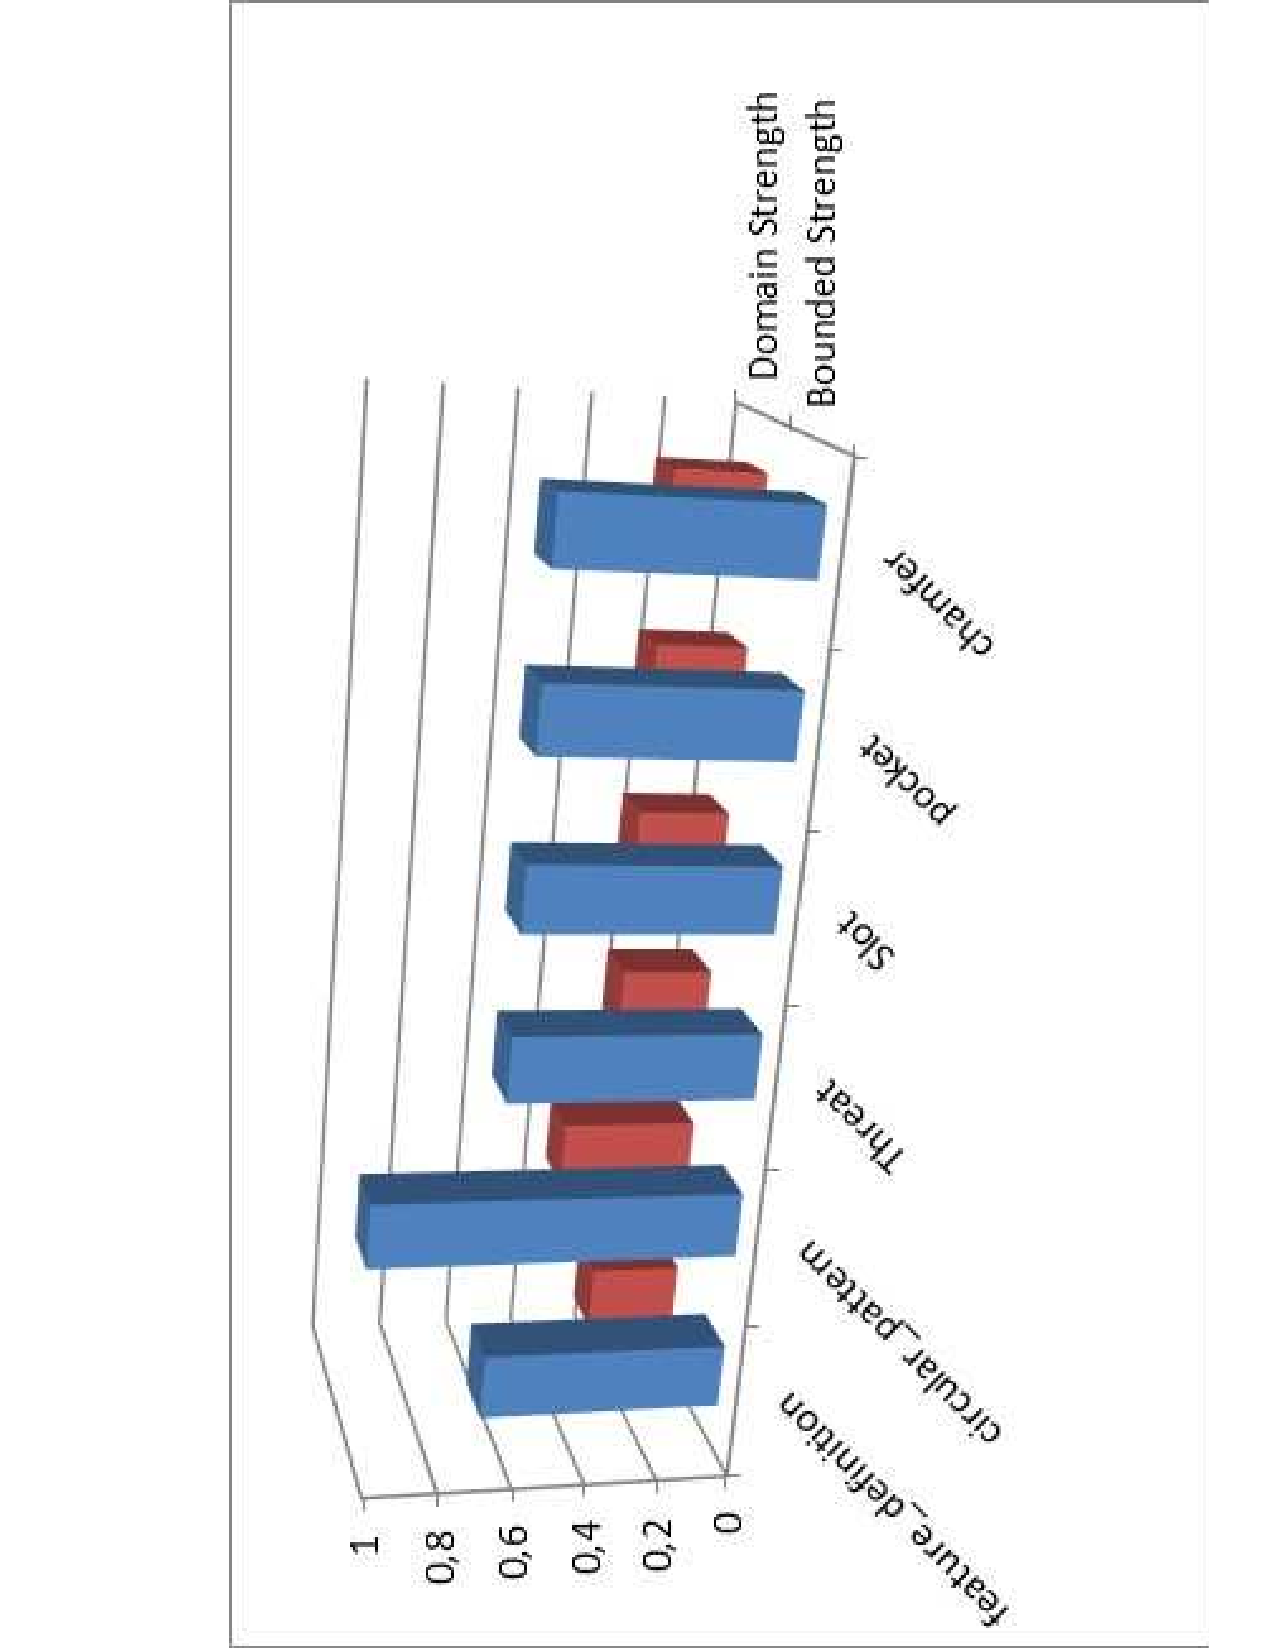
\includegraphics[scale=0.5, angle=-90]{figure-chapterIV/fig4-22.pdf}\\
	\caption{Hypermodule of Features}
	\label{figure4-22}
\end{center}
\end{figure}

Fig. \ref{figure4-23} shows the hyperontology of Features, where concept \texttt{Features} is the  root concept in this ontology. These Features mostly apply to mechanization procedures. 


\begin{figure}
\begin{center}
	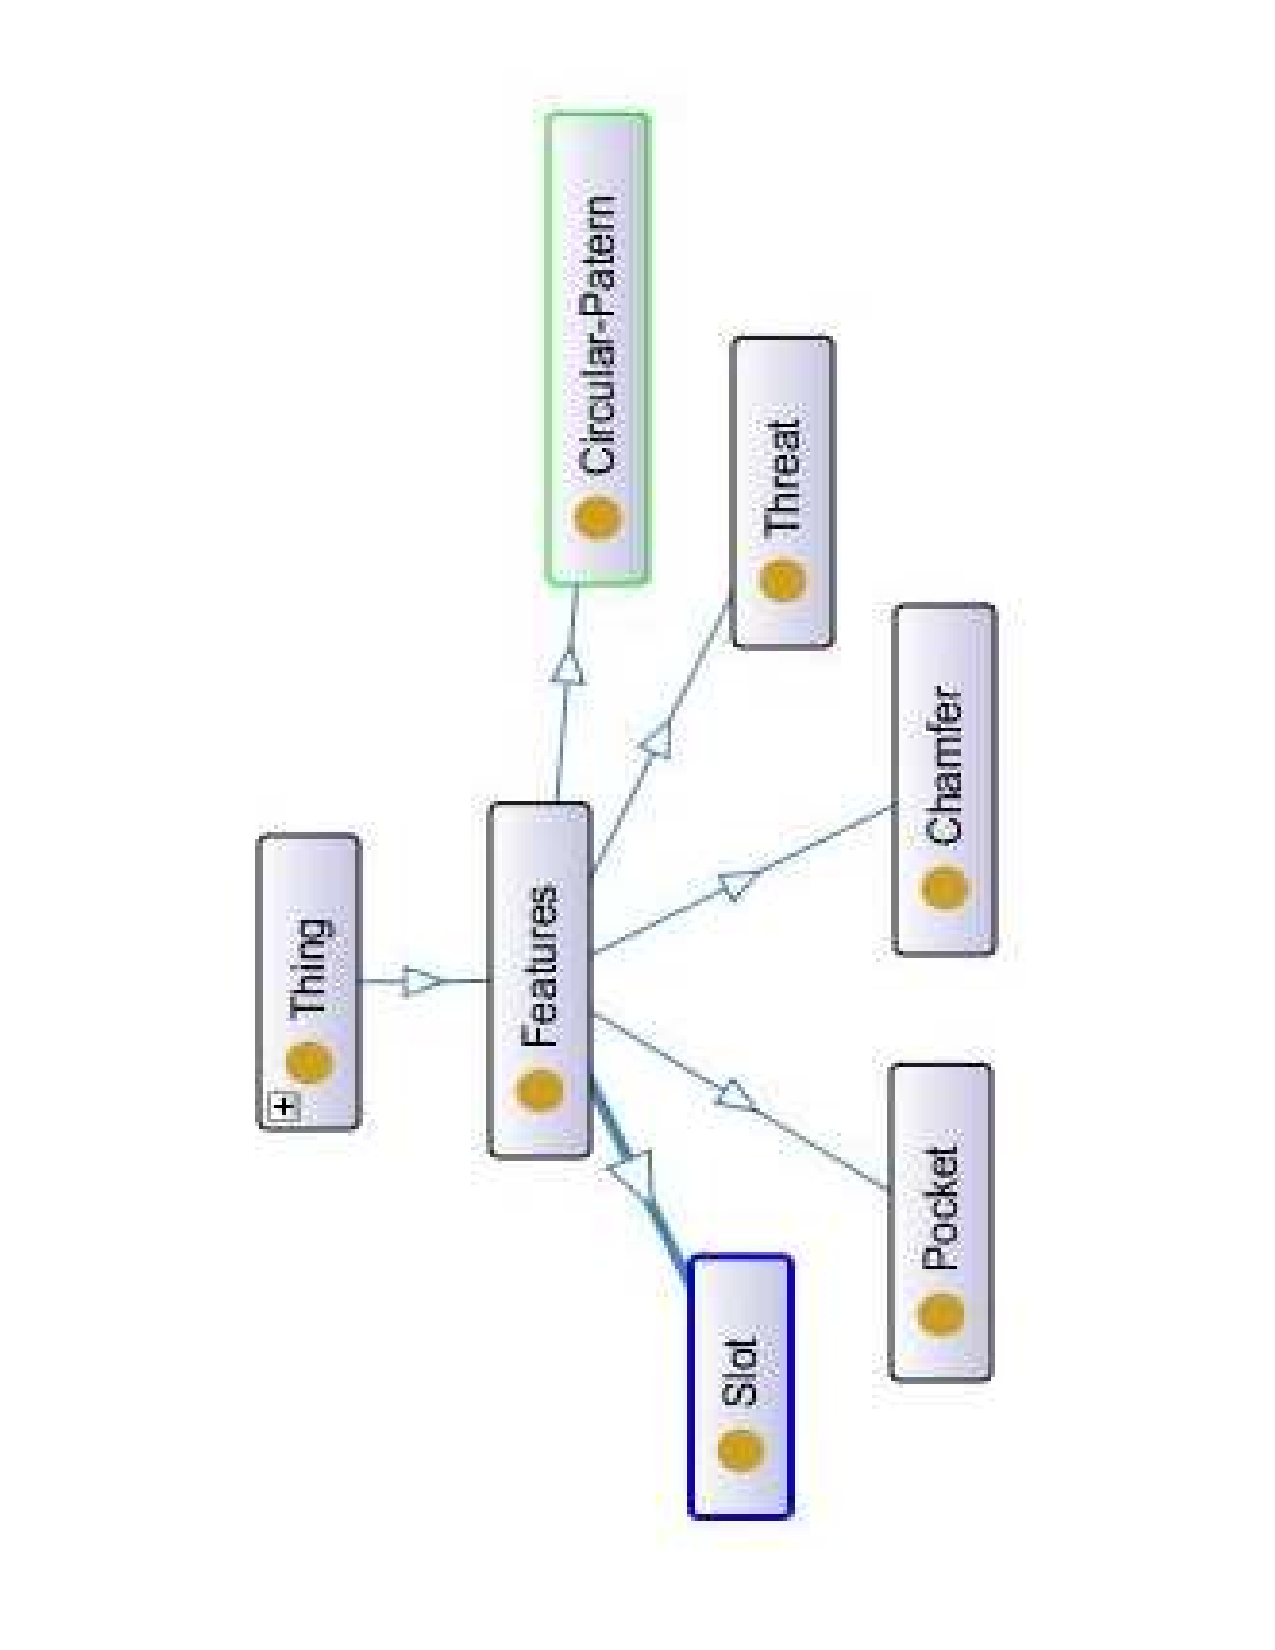
\includegraphics[scale=0.5, angle=270]{figure-chapterIV/fig4-23}\\
	\vspace{-40}
	\caption{Hyperontology Features}
	\label{figure4-23}
\end{center}
\end{figure}

Continuing with the description of the hyper modules obtained by the execution of the proposed algorithm, we obtained \texttt{Resource, Machine, Tool, Lathe} and \texttt{Drill} concepts. All these concepts were  found in the MASON and OntoMoPS ontologies, while in OntoSTEP only 2 of them were found. 

If we return to the results previously obtained during the evaluation of the Hyper module of Features, we found that the features and the resources to \cbstart get the features manufactured on the raw material \cbend are present in the MASON ontology as well. For instance, with a Lathe we can make circular patterns. This is a commonality that until now has only appeared in this case. Where MASON appears with common concepts that relates two pairs of ontologies: a first pair OntoStep-MASON where the concept \texttt{Feature} is developed, and a second pair MASON-OntoMoPS where the concept \texttt{Resource} is developed. Some of the resources mentioned in the latter pair are required as machinery for manufacturing the Feature mentioned in the former pair. 

In this vein, Fig. \ref{figure4-24} contains the result of applying the BS and DS parameters to the network where these \texttt{Resource} and \texttt{Drill} concepts have a BS of 1, while the others have a BS of 0.66. Besides having the same BS value, \texttt{Resource} is more general than \texttt{Drill}, where \texttt{Drill} is a type of machining. The resulting ontology is shown in Fig. \ref{figure4-25}.


\begin{figure}
\begin{center}
	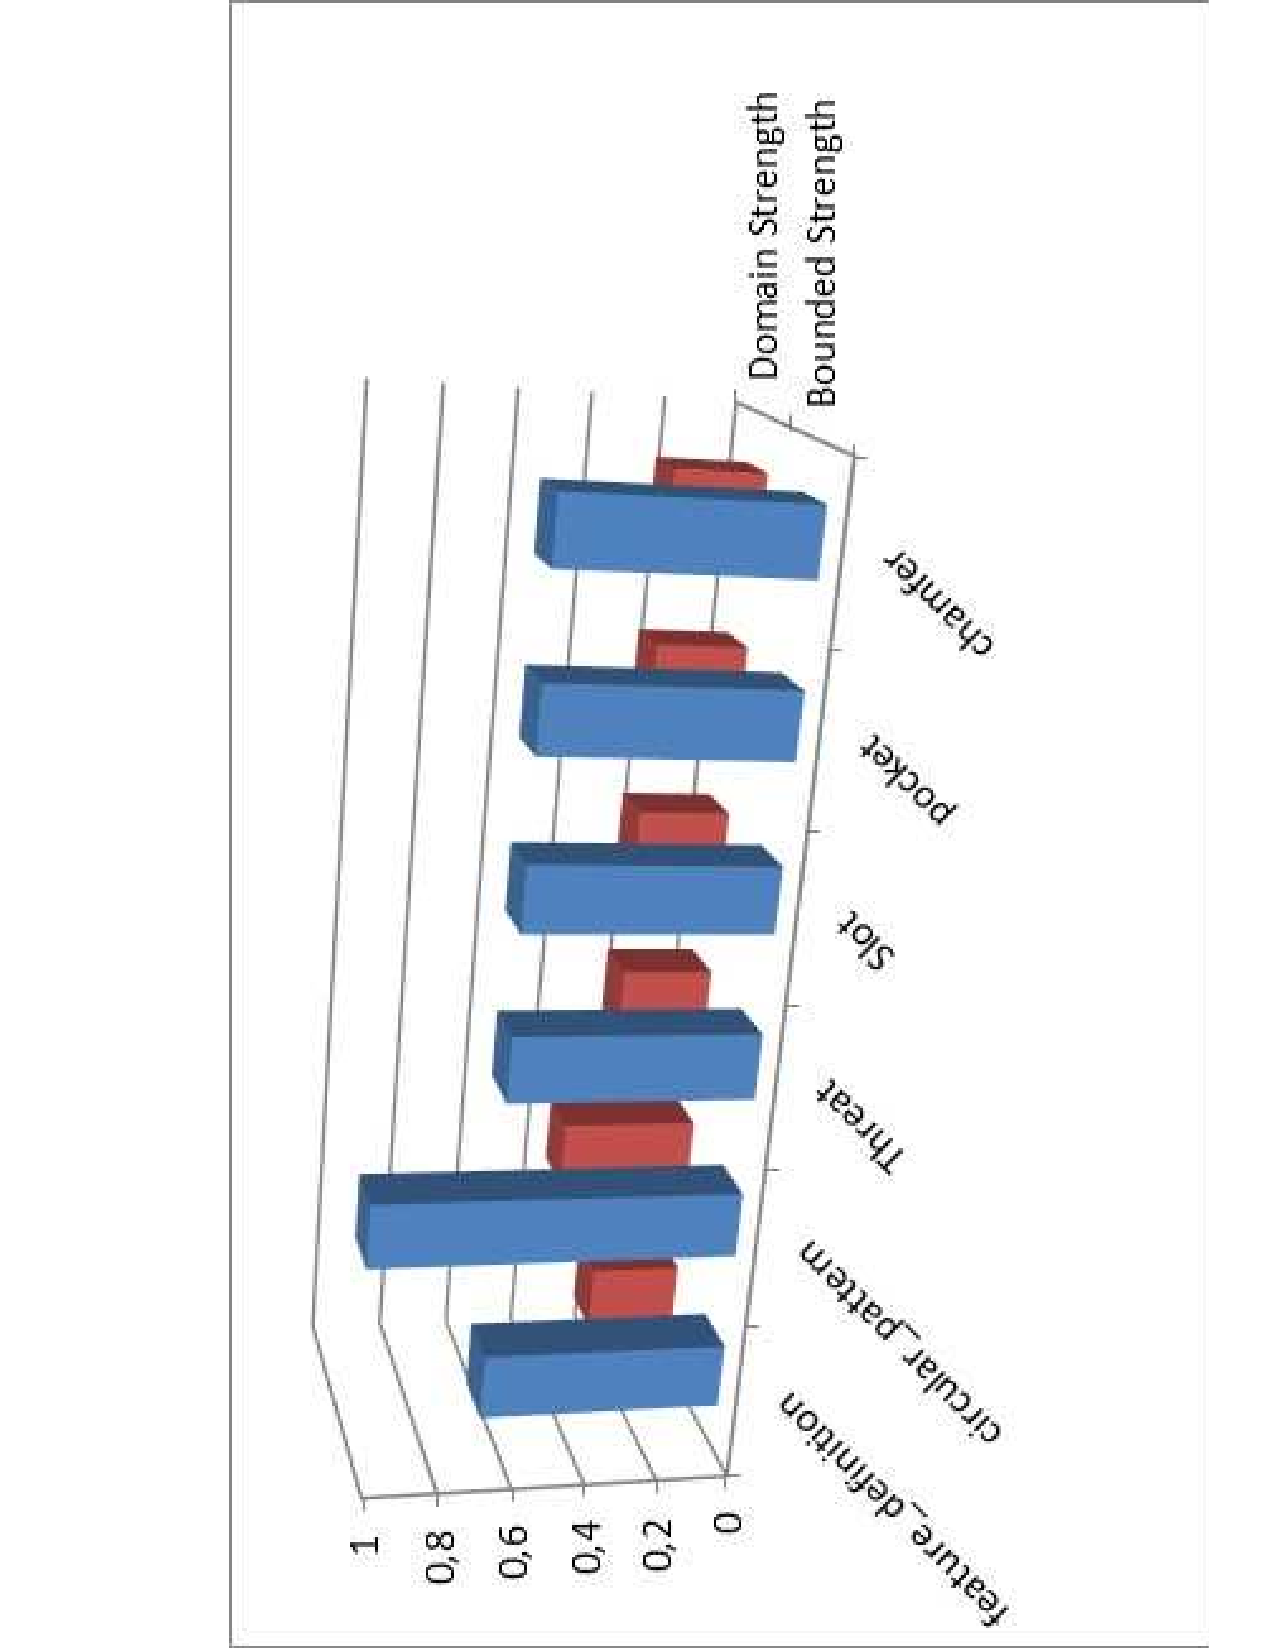
\includegraphics[scale=0.5, angle=-90]{figure-chapterIV/fig4-24.pdf}\\
	\caption{Hypermodule Resources}
	\label{figure4-24}
\end{center}
\end{figure}

\begin{figure}
\begin{center}
	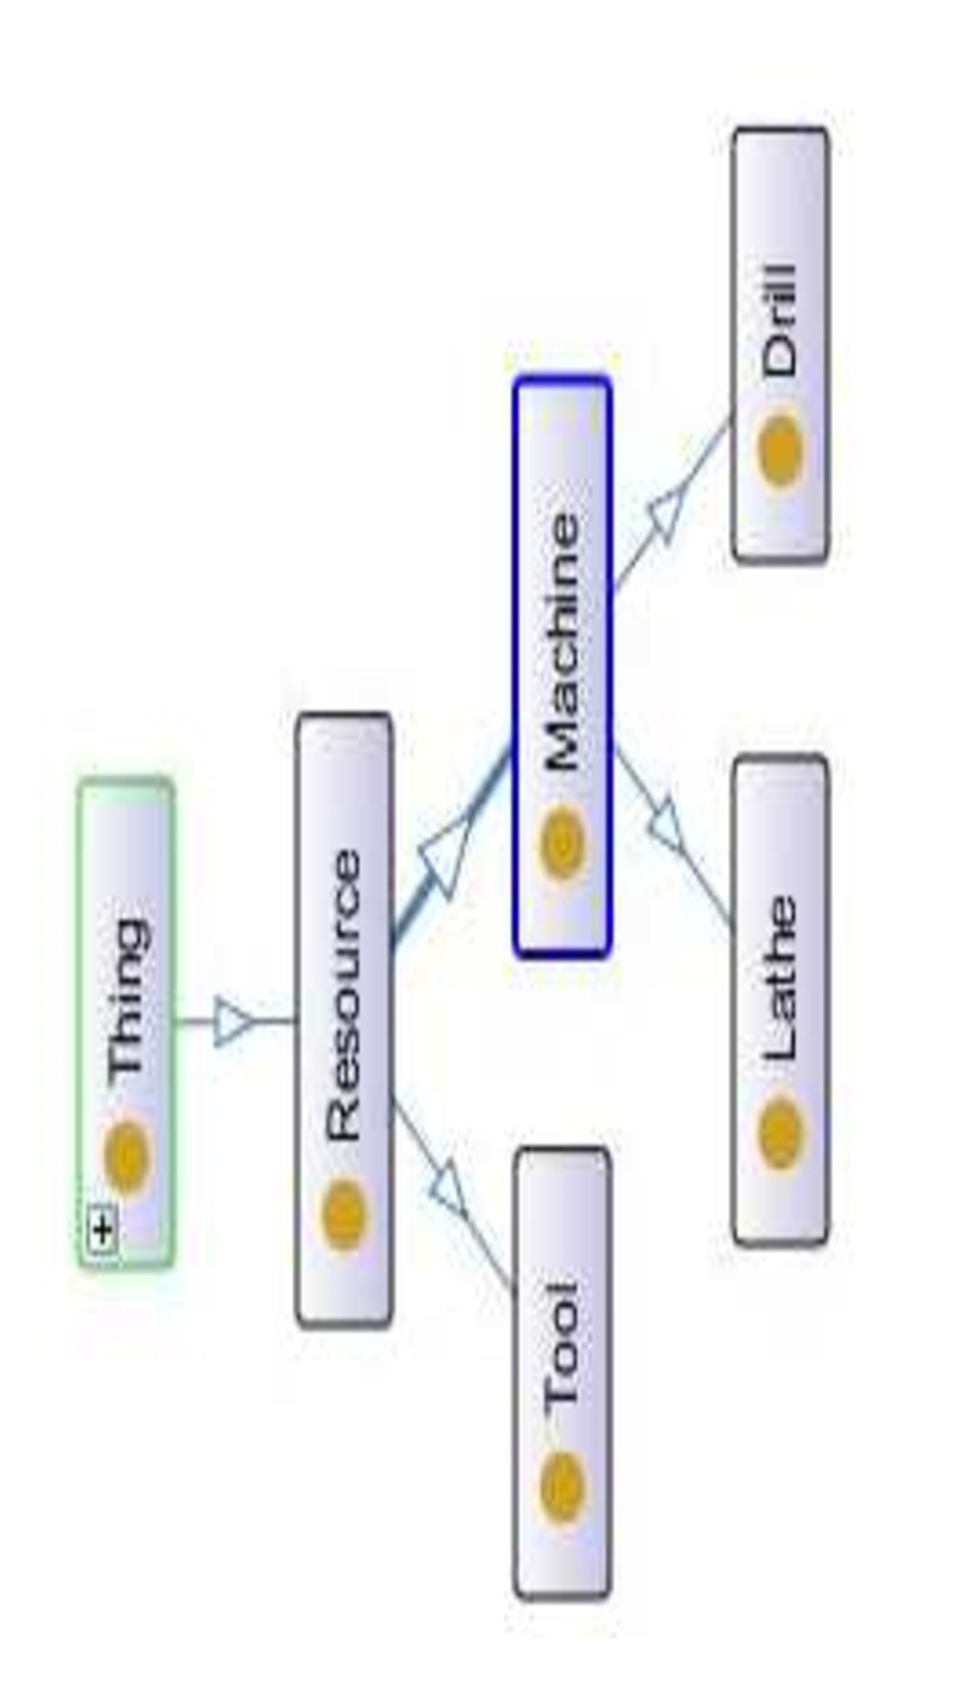
\includegraphics[scale=0.5, angle=270]{figure-chapterIV/fig4-25}\\
	\vspace{-40}
	\caption{Hyperontology of Resource}
	\label{figure4-25}
\end{center}
\end{figure}

\subsubsection{Hyper module of Curve}\label{subsubsection4.2.5.5}


The last hyper module we found following the proposed algorithm shown in Fig.\ref{figure4-15}, corresponds to the  \texttt{Line, Conic, Curves, Circle, Hyperbola, Ellipse} and \texttt{Parabola} concepts. The mappings found correspond to 2 ontologies only, those are OntoStep and BeyondSTEP, while the other ontologies of the network remain isolated. 

In this case, the BS of every concept is equal to 1, meaning that every concept is in all ontologies of the boundary, and  DS is equal to 0.25 which means that these concepts make up less than 25\% of the ontologies. Fig. \ref{figure4-27} introduces the categorization of these concepts. Considering \texttt{Line} and \texttt{Conic} as \texttt{Curves}, and \texttt{Circle}, \texttt{Hyperbola}, \texttt{Ellipse} and \texttt{Parabola} as \texttt{Conics}. 



\begin{figure}
\begin{center}
	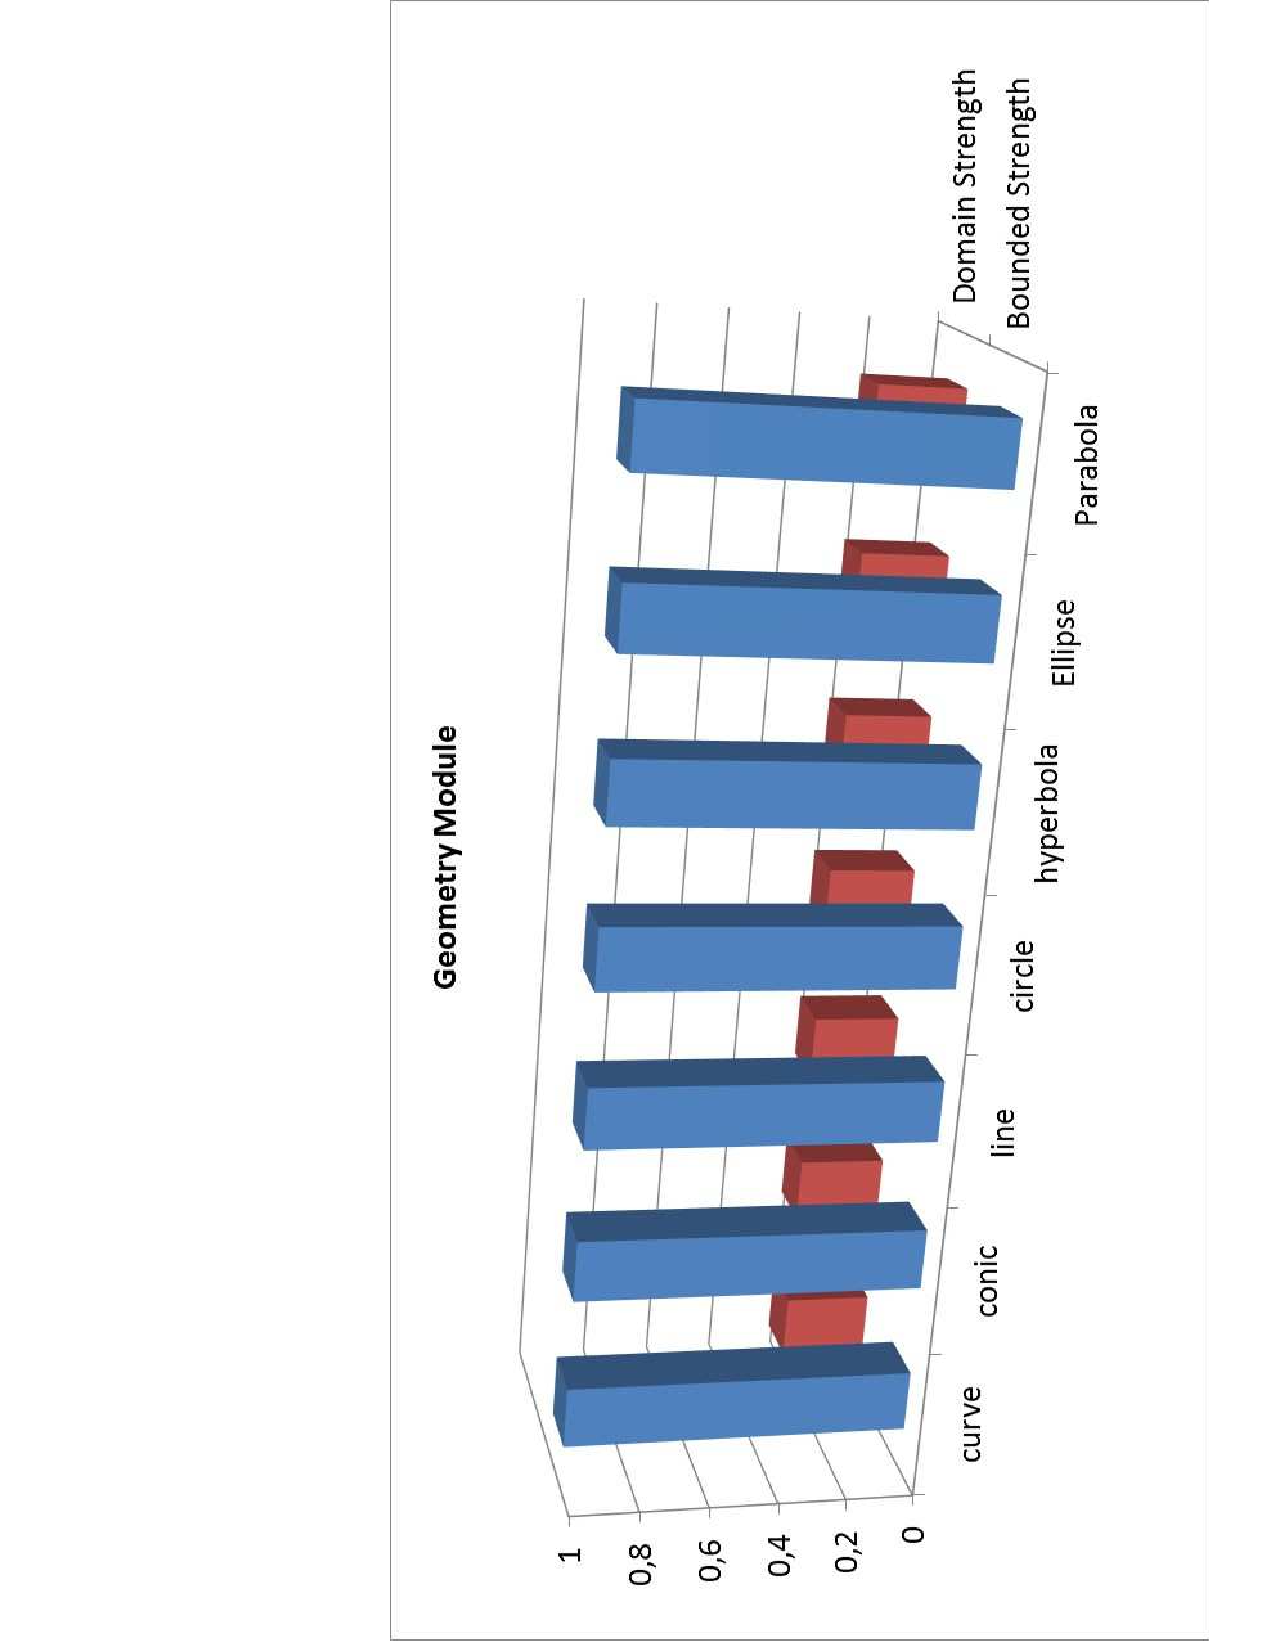
\includegraphics[scale=0.5, angle=-90]{figure-chapterIV/fig4-26}\\
	\caption{Geometry Hypermodule}
	\label{figure4-26}
\end{center}
\end{figure}





\begin{figure}
\begin{center}
	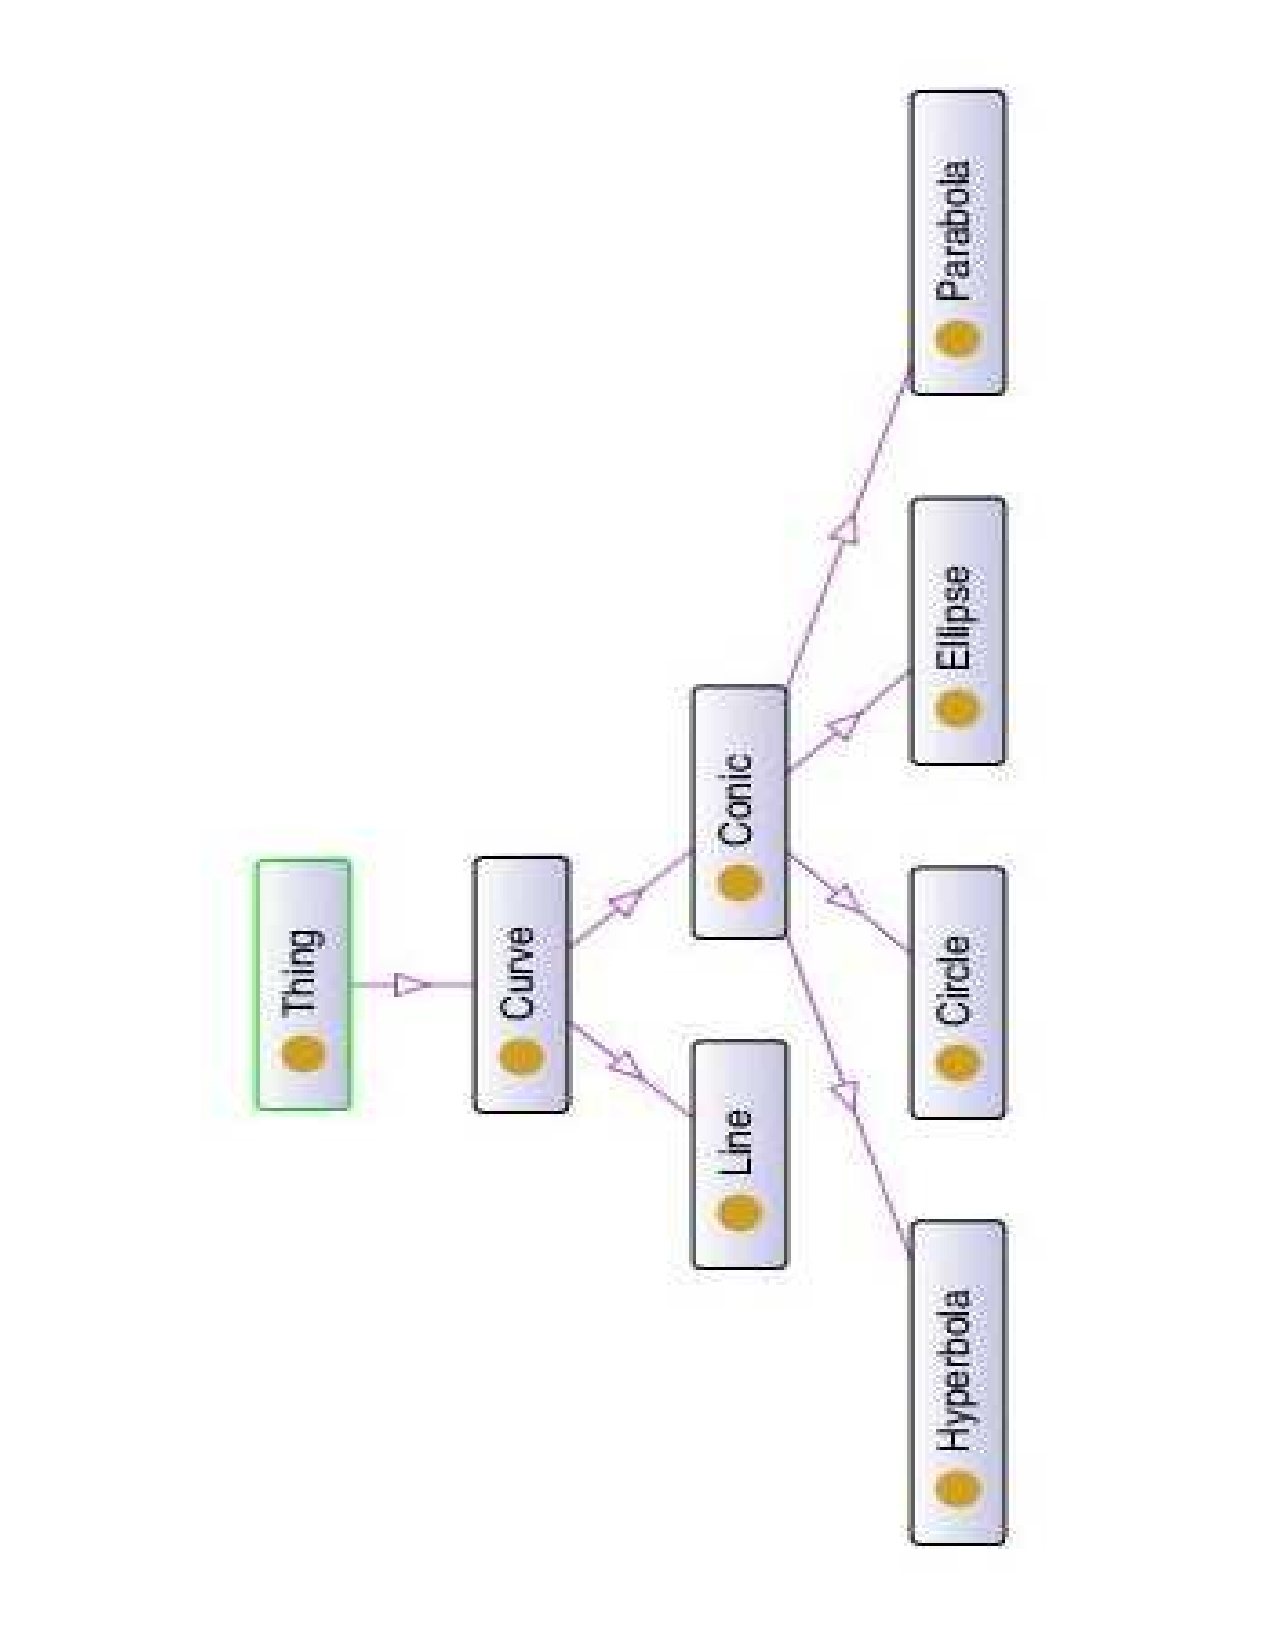
\includegraphics[scale=0.5, angle=270]{figure-chapterIV/fig4-27}\\
	\vspace{-20}
	\caption{Geometry Ontology}
	\label{figure4-27}
\end{center}
\end{figure}




With the hyper module of curves we complete the application of the algorithm presented in Fig.\ref{figure4-15}. The obtained hyper modules now have to be integrated with the network of ontologies shown in Fig.\ref{figure4-10}. At this point it is worth remarking that our hyper ontology will be formed by some hyper modules, and in the case of our algorithm we have proposed two types, mono-modules and multi-modules. This hyperontology is an interoperability artifact that is located on top of the network of ontologies, and the mappings obtained from the algorithm serve as hyperlinks. With these notions we proceed to summarize our findings in Fig. \ref{figure4-28}, which at the same time serves as the representation of our complete hyperontology. At the bottom of the figure, we show the network of ontologies from Fig. \ref{figure4-10}. At the top, every hypermodule is drawn; the mono-modules containing only one concept in yellow, and the multi-modules containing several concepts in black. 


This figure illustrates the complexity of representing a domain of discourse, concretely considered in this case for manufacturing. For instance, a product can be goods or  service. If we choose to represent goods, some products could be represented as a CAD drawing, while others, like liquids, cannot be represented in this way. In the case of the resulting hyper ontology, it will only serve for representing solids according to the Features terminology it contains. \textbf{why?}

Furthermore, it is likely to find at least two   ontologies with restricted scope. Those include, for example, the Sweet Ontology, which only has a mapping through the hyper module of \texttt{Unit} toward 4 more ontologies, and BeyondStep which has two mappings through the concepts \texttt{Features} and \texttt{Geometry} toward 3 more ontologies. Such mappings allow us to extend those apparently restricted scope  ontologies through these mappings toward more complex ontologies.

Moreover, if we consider ontologies with an apparently  different scope in a manufacturing domain, like MASON (manufacturing) and GoodRelations (ecommerce), their commonalities allow certain information exchange through this network, in this specific case information about the product. In contrast, information of the manufacturing process is not exchangeable because these concepts are not part of GoodRelations terminology. 

Here we complete the activities of modularization planned in our methodology, before proceeding onto the steps of Axiomatization and Heterogeneity. Moreover in Section \ref{section4.4} an application example with the obtained hyper ontology in Fig. \ref{figure4-28} will be introduced. 



\begin{figure}
\vspace{-10}
\begin{center}
	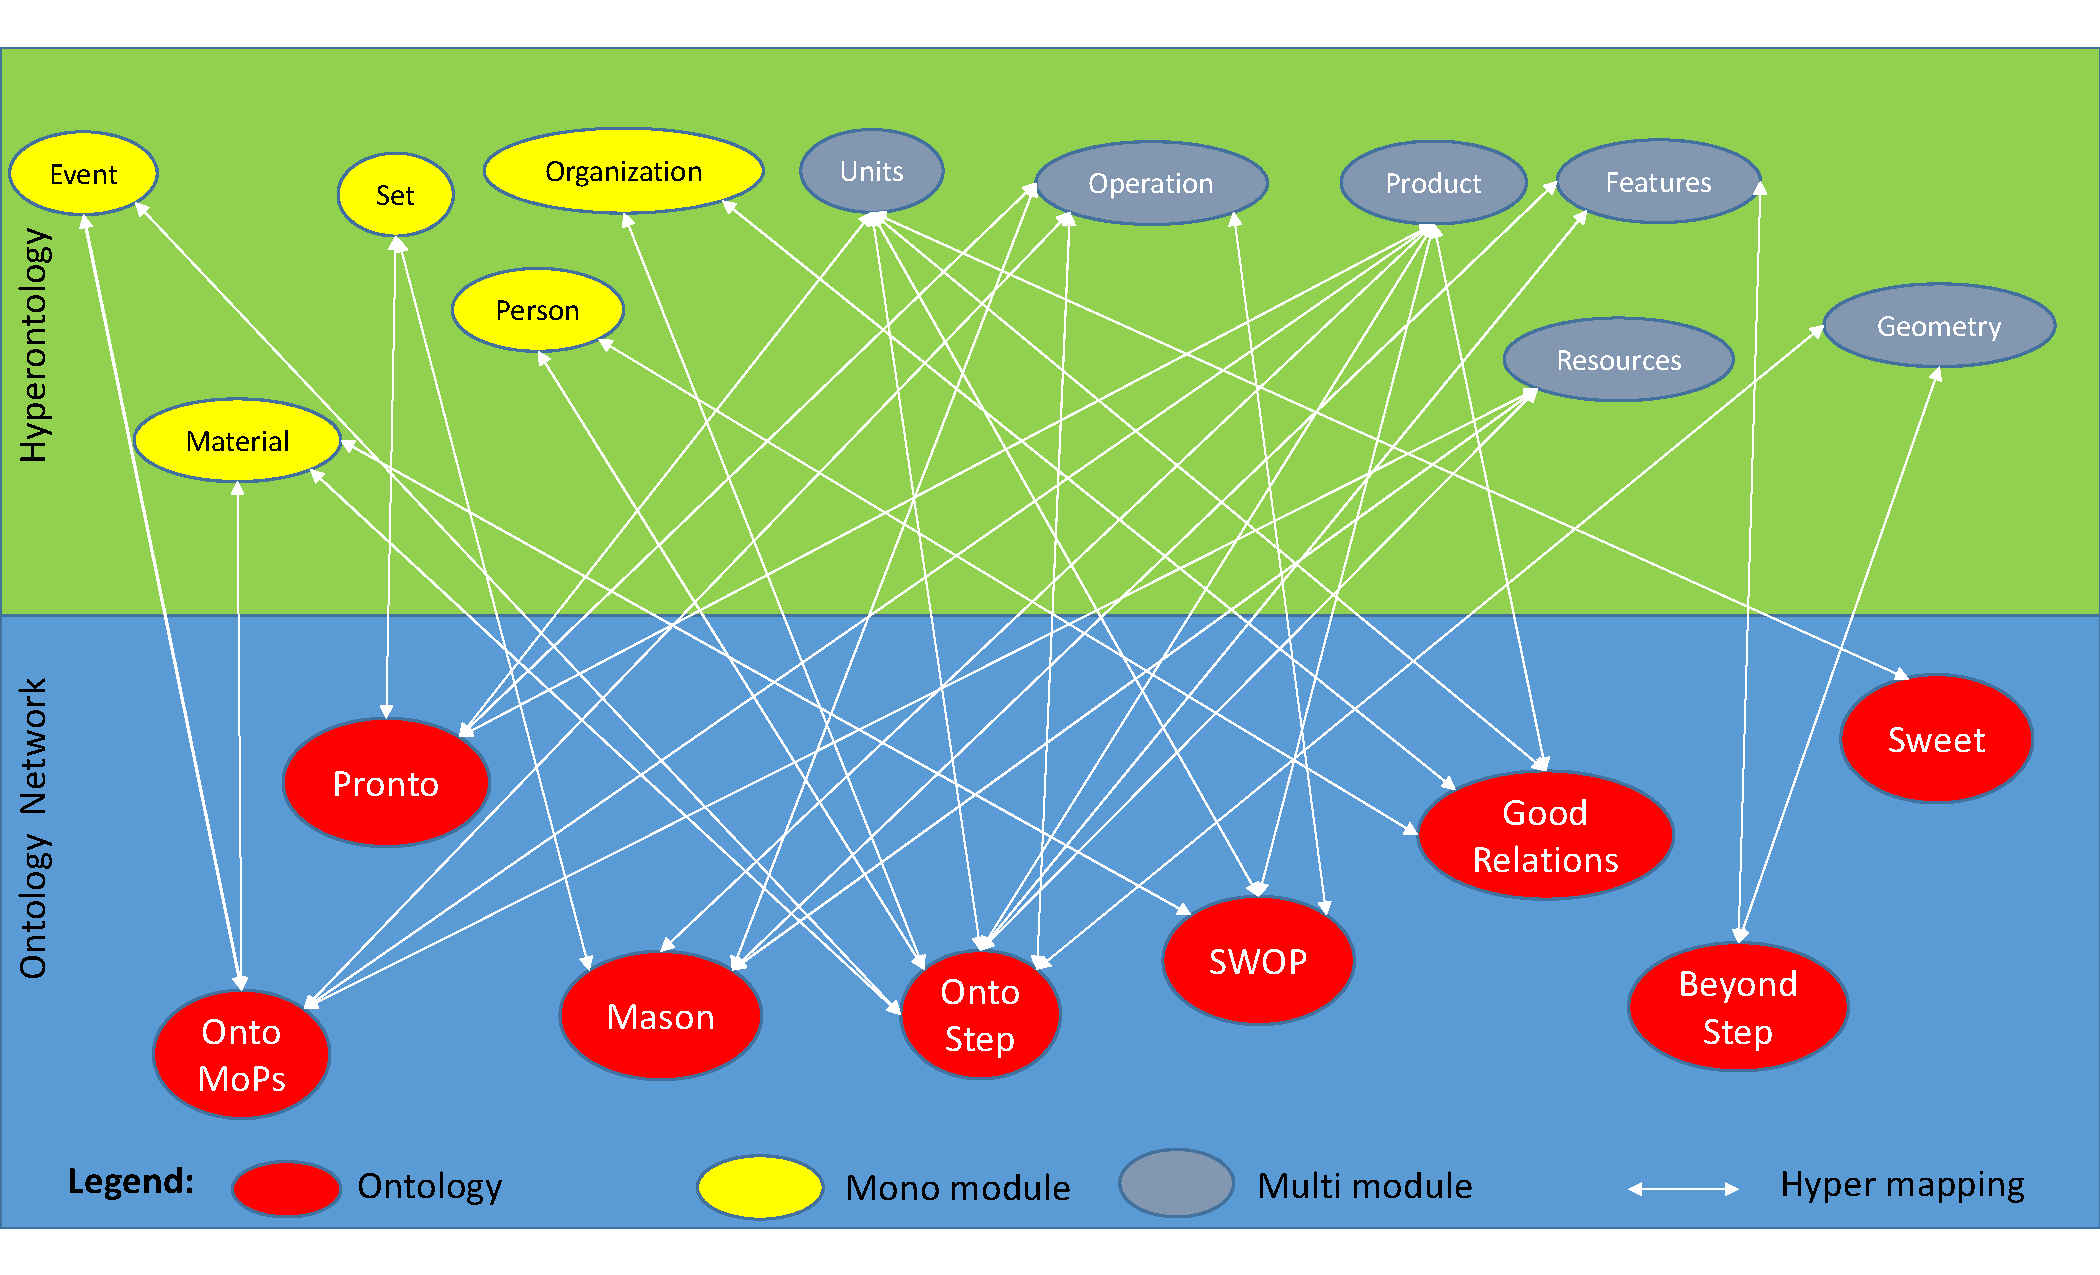
\includegraphics[scale=0.6, angle=90]{figure-chapterIV/fig4-28.pdf}\\
	\caption{Resulting Hyper ontology}
	\label{figure4-28}
\end{center}
\end{figure}



\section{Between Light Weight and Heavy Weight Ontologies}\label{section4.3}


Continuing with the development of our methodological approach as depicted in Fig. \ref{figure3-1} of our Proposed Methodology, we have to proceed to determine whether or not heavyweight ontologies are required, following the procedure indicated in Subsection \ref{subsection3.2.2}. There we defined the metric $al$ which lets us know the average of defined concepts in an ontology; moreover we proposed a criterion to determine whether or not a heavyweight ontology is required in our application. 

Therefore, first it is necessary to determine whether heavyweight ontologies are needed. As shown in Section \ref{subsection3.2.2} this depends of the application requirements. Thus we have to consider the following aspects: All ontologies considered in Fig. \ref{figure4-28} were written in  OWL and OWL is based in Open World Assumption   (See Subsection \ref{subsection2.2.3} in Chapter \ref{chapter2}), where an individual is considered as a member of a concept, and it is necessary to provide a specific definition of the concept or restrictions through  closure axioms. These closure axioms allow the classification of individuals as members of a class.     This classification feasibility is a fundamental characteristic in Ontological Engineering.  

To illustrate this classification need in engineering, we can   consider the AFR approach described in Subsection \ref{subsection2.1.1}, which consists in recognizing certain features from CAD files. In the hyper module of Features, some of the most common mechanical features mentioned in the literature are included. When AFR is executed on a digital design, the following classification takes place: a group of geometrical elements receive mechanical and manufacturing semantics when they are classified according to some specific features, defined by a set of axioms. 

There is also the FMS approach, which, according to the description we provided in Subsection \ref{subsection2.1.3} (Chapter \ref{chapter2}), assumes that with an intensive utilization of Numeric Control (NC) techniques, automatic materials handling and computer hardware and software, the manufacturing time for customizing goods should be considerably reduced. Here a classification is also involved whenever from a group of resources (machinery) we have to decide which can fulfill our manufacturing requirements   and how they should be organized in the factory. 

Another example can be provided considering market segmentation principles. In this case customers are divided into groups or segments, based on their preferences, and products can be assigned to certain segments of customers according to the satisfaction levels they are able to provide for each group or segment. 

Through the description of the three common scenarios mentioned above, we can consider that heavyweight ontologies are required in such scenarios in order to enable classification. 

After defining the requirement of heavyweight ontologies for manufacturing, equation \ref{eq4.2} proposed in Subsection \ref{subsection3.2.2} is applied. This formula allows us to obtain the relation between defined and primitive concepts in an ontology, with the intention of defining the purpose of the evaluated ontology, controlling vocabulary or classification.  Thus, we can confirm our position that manufacturing ontologies should have mostly defined concepts with the intention of making such ontologies usable.   



\begin{figure}
\begin{center}
	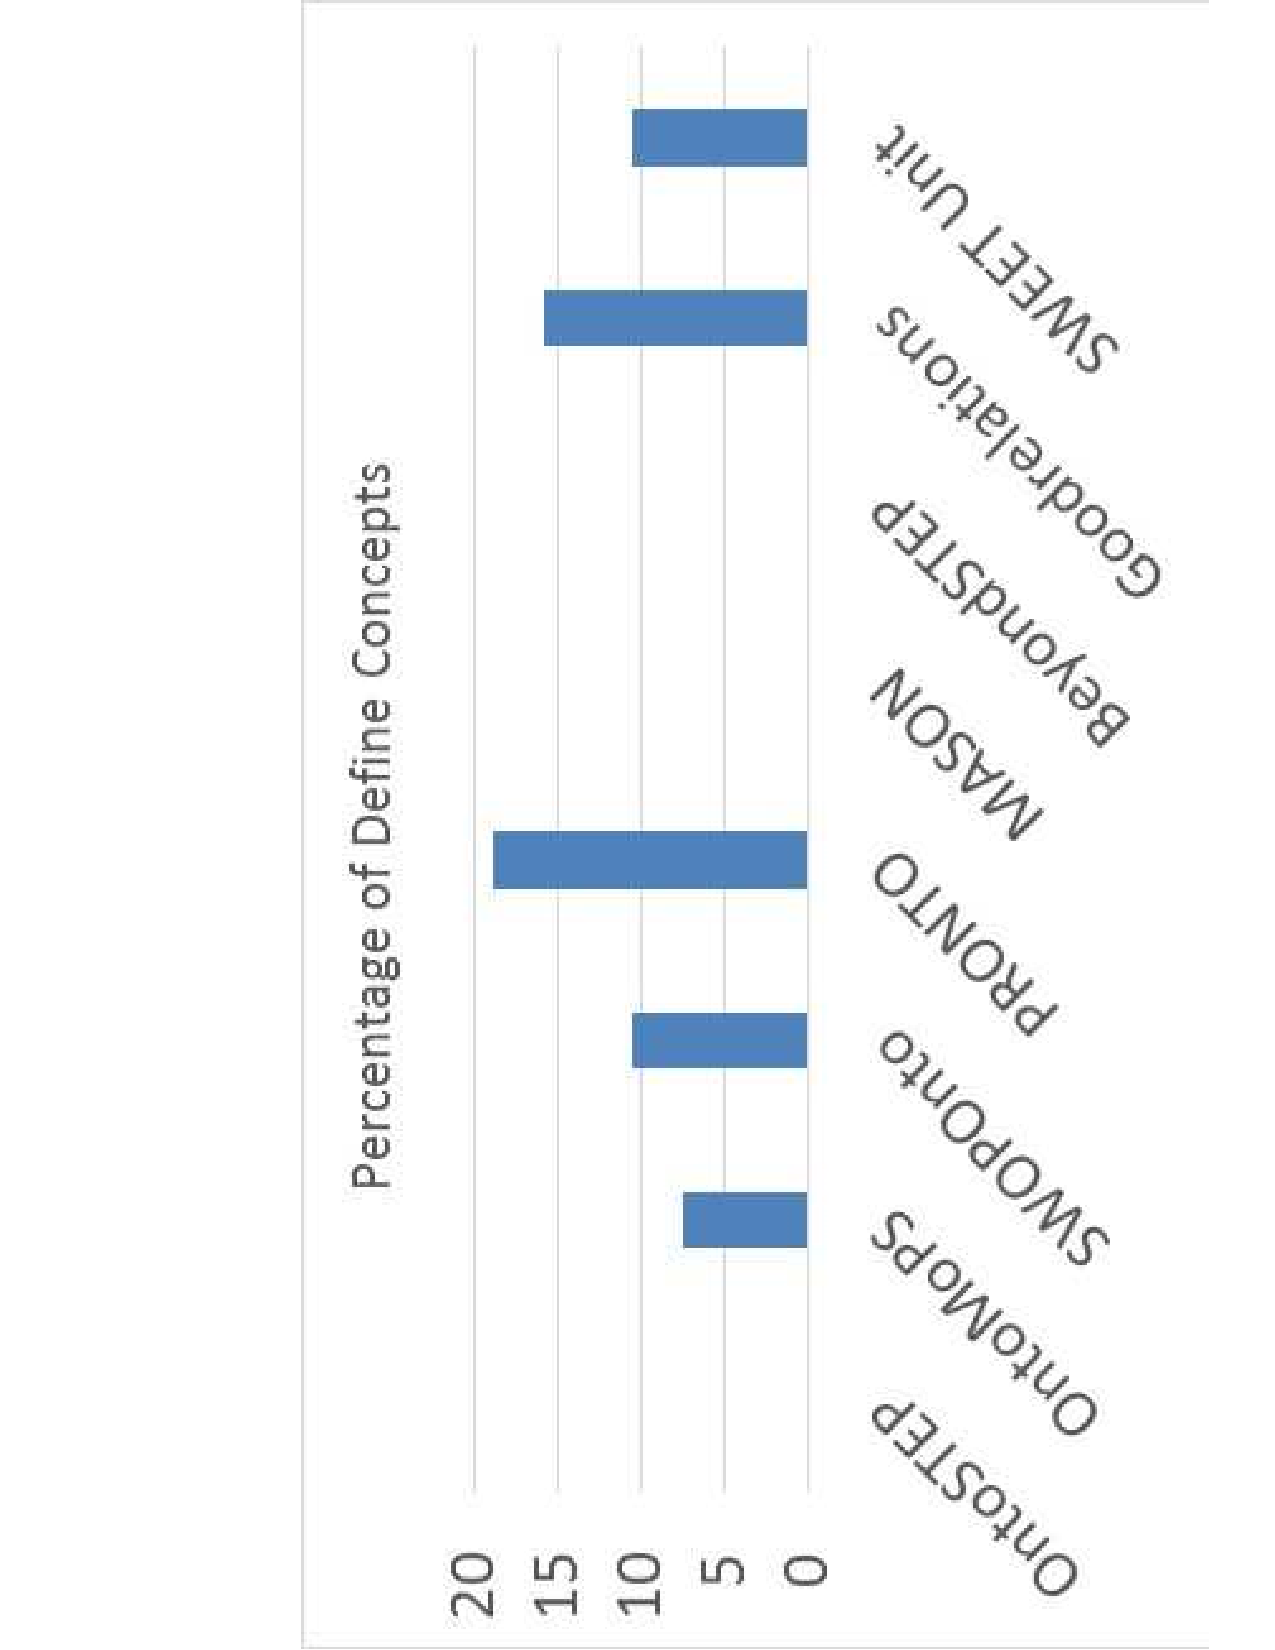
\includegraphics[scale=0.5, angle=-90]{figure-chapterIV/fig4-29.pdf}\\
	\caption{Defined    Concepts in Network}
	\label{figure4-29}
\end{center}
\end{figure}



Fig. \ref{figure4-29} presents a view of the presence of defined concepts in the network of ontologies under evaluation. From the 8 ontologies considered, 5 have some defined concepts in different proportions, varying from 7 to 19\% of the total. Here, an apparent contradiction appears: that is while in the previous paragraph we stated that heavyweight ontologies are needed for applications like AFM and FMS, Fig. \ref{figure4-29} shows that in many ontologies like OntoSTEP, MASON and BeyondStep, there are no defined concepts. However, in other ontologies like PRONTO and GoodRelations there are defined concepts present,  ranking from 15\% to 19\%.

To relate usability with heavyweight ontologies, we consider the result obtained in the case of the GoodRelations ontology, because from ontologies mentioned in Fig. \ref{figure4-29} only this has shown use outside of academia. This ontology is used in some of the most important   search engines and it is well accepted in the ecommerce community \citep{hepp_references_2013}. Moreover it has an appropriate platform for making it available to a community of users. Approximately 16\% of this ontology is made up of defined terms, and its basic use consists in allowing goods selection according to user criterion. 

Another necessary consequence of this result can be concerning OntoStep and BeyondStep. These ontologies were considered as CAD ontologies   in Subsection \ref{subsection2.2.1}. From the percentage of defined concepts in OntoStep and BeyondStep shown in Fig. \ref{figure4-29},  we can assure they are lightweight ontologies because they contain no defined concepts. Thus, if we wish to perform AFR, many terms in these ontologies shall be defined, in other words OntoStep and BeyondStep, are incomplete for AFR and FMS, and the ontological engineer will need to perform additional work defining concepts to make these ontologies usable with this type of tasks. 

In this subsection we discussed axiomatization requirements, and showed that from the list of ontologies we have evaluated, many were lightweight. This result does not make these ontologies useless, but it does make necessary additional work to define appropriate concepts in order to make them usable in tasks like FMS and AFR. For these tasks, in our opinion, heavyweight ontologies are required. 

Following with our methodology shown in Fig. \ref{figure3-1}, we proceed to the heterogeneity activities. However as we will later demonstrate, this decision is based on application requirements, so in the next section we present an application example where domain requirements will take us back to heavyweight ontologies in order to fulfill the application goals.  



\section{Implementing Heavyweight Ontologies}\label{section4.4}


At the beginning of Chapter \ref{chapter2}, CAx systems were introduced as an attempt to improve manufacturing automatization, optimization and acceleration levels. For example, during this research we observed how AutoDesk developed its Drawing Exchange Format (DXF), a \textit{de facto} standard for the exchange of CAD data facilitating reading a CAD design previously deployed using other software tools such as AutoCAD® of AutoDesk. A detailed explanation of this standard can be found in the DXF Reference Manual \citep{autodesk_dxf_2009}.  This standard defines geometric primitives such as LINE, CIRCLE, ARC and ELLIPSE entities. A group of codes is specified for each one, indicating what type of data value or feature they follow. It is also possible to extract from a DXF file descriptions of text, surfaces, color and texture, but the information on solids is encrypted \citep{choi_exchange_2003} and limits data information exchange among CAD design. In the same way, the work flow starting from the manufacturing design is restricted to the AutoDesk family of products. Therefore, besides the important advantage of CAx systems, these technologies have shown patent shortcomings, one of these is the lack of interoperability.  This interoperability issue occurs because most vendors allow interoperability along the workflow of the tools they offer, but interoperability between tools of different vendors tends to be limited in some way.


In Subsection \ref{subsection2.4.1} we stated that in recent years there has been a movement toward the utilization of the ontological approach in engineering applications for the representation of  CAD models to capture feature semantics and to use such models among different systems maintaining the designer’s purpose. \cite{abdul-ghafour_common_2007} presented an architecture for a Data Exchange among different CAD software tools, where ontologies are proposed to represent terminologies of several commercial CAD software tools, and a main ontology would serve as a Common Design Feature Ontology. \cite{abdul-ghafour_common_2007} proposed to write and store ontologies of each CAD system using OWL, generating ontologies of such systems.   These ontologies have to be mapped into a Common Design Ontology to make them interoperable accross different software applications. Similarly, \cite{andersen_building_2007} proposed an ontology of CAD model information; this proposal is described as an introduction to ontologies and shapes representation and deals only with the STEP standards as also done by \cite{abdul-ghafour_common_2007}, presenting a taxonomy of terminologies included in the STEP standard. 

In contrast, building on the proposal of \cite{abdul-ghafour_common_2007}  we  have proposed a different data exchange approach \citep{ramos_ontological_2010}. There, intermediate ontologies were avoided and a general CAD terminology was used without adopting specific standard CAD terminology. We considered this could be a disadvantage for an approach that, on the one hand, claims to be ontological while, on the other hand, it is only being related to one CAD standard. Fig. \ref{figure4-30} presents our first attempt to deal with this interoperability issue in CAD.  In this figure, we exemplify the architecture with DFX and IGES standards. Consequently, in the figure  there are four parsers: \cpstart Two preprocessors parsers for exchanging DFX into OWL, and two postprocessors parsers for exchanging OWL in DFX, similarly in IGES\cpend. As soon as a standard is converted into OWL, the reasoning framework of the Semantic Web (Fig. \ref{figure2-7}) becomes available. With a CAD design based on OWL, it is possible to provide reasoning on the CAD ontology, in order to exchange from one format to another. 


\begin{figure}
\begin{center}
	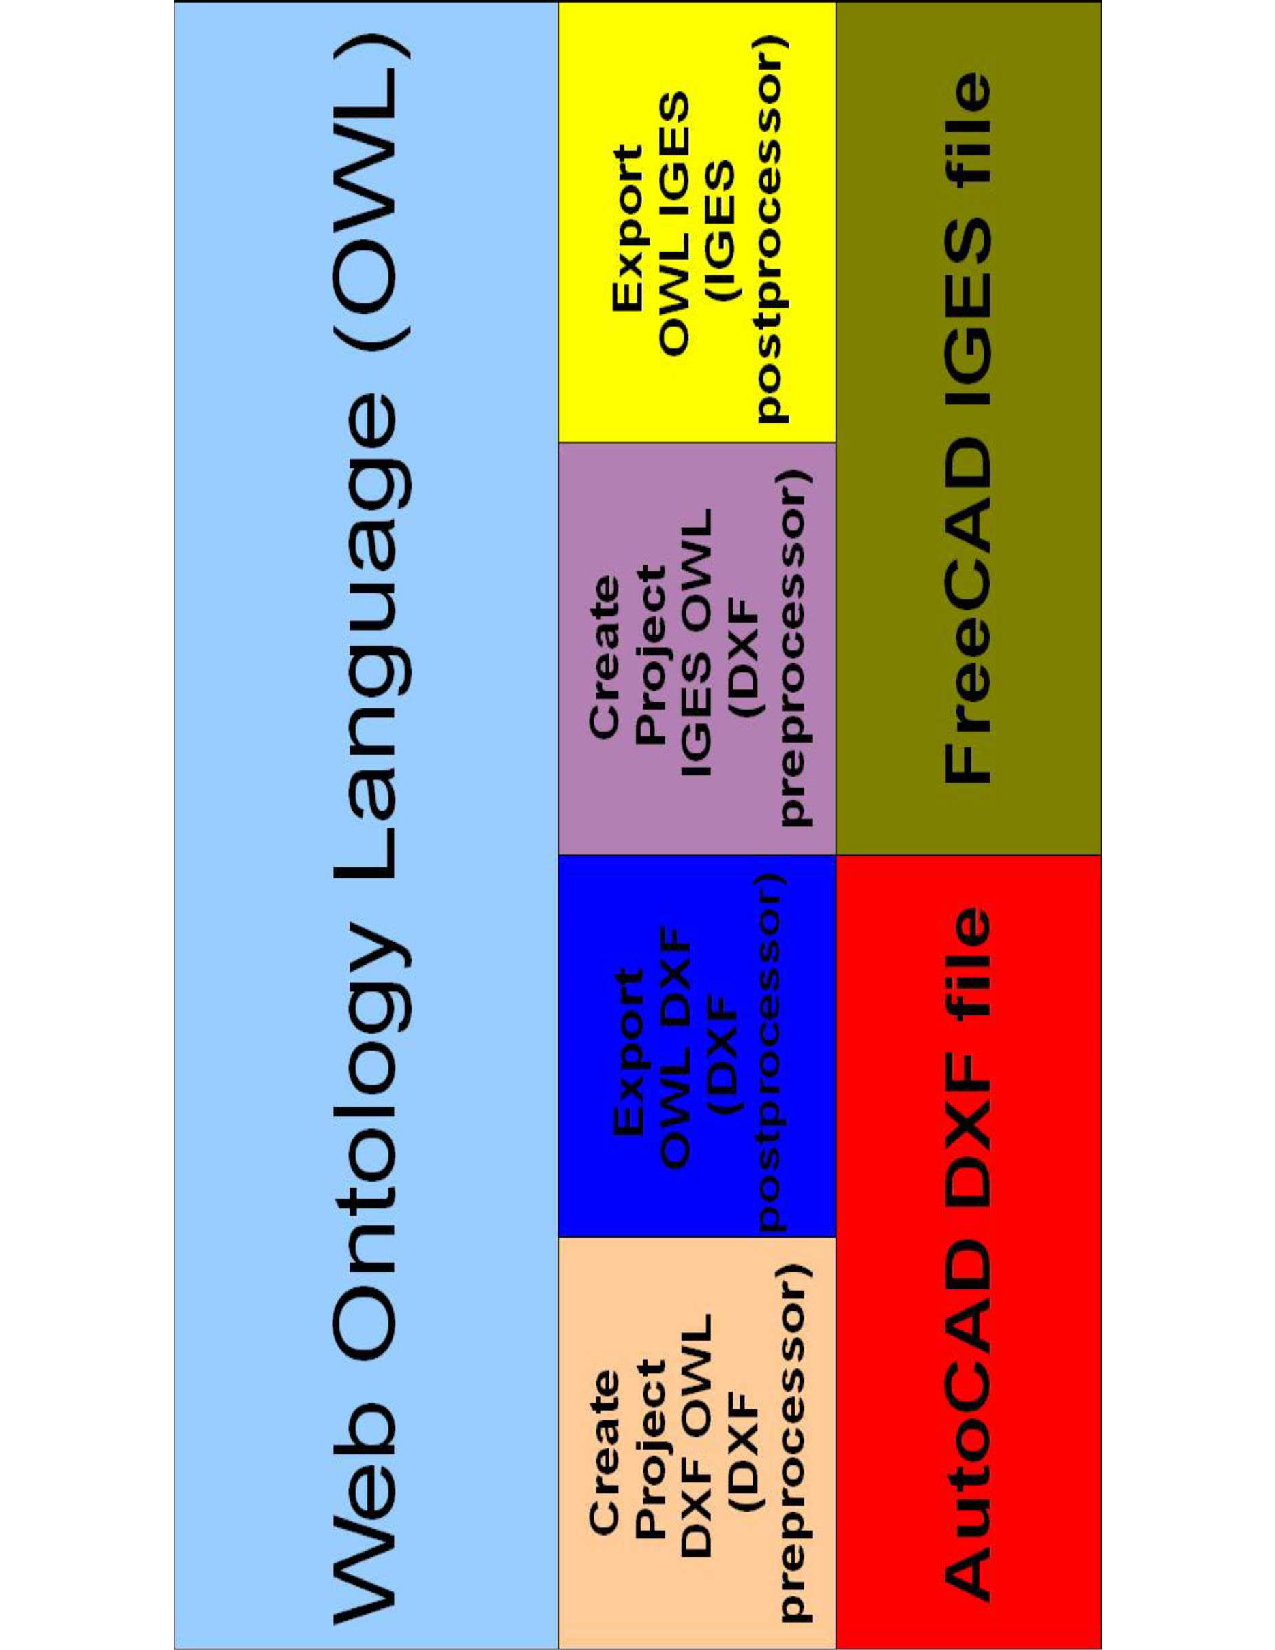
\includegraphics[scale=0.5, angle=270]{figure-chapterIV/fig4-30}\\
	\caption{OWL Based CAD   Exchange Framework}
	\label{figure4-30}
\end{center}
\end{figure}

In order to assess the usability of the Semantic Web in manufacturing, other uses additional to exchanging data of specific CAD formats like DXF and IGES shall be considered. \cpstart The issue of representing and reusing the designer’s purpose in a CAD designs is one of those\cpend. This issue is illustrated in Fig. \ref{figure4-30} and Fig. \ref{figure4-31}. The former shows a common mechanical piece used in engineering, better known as a flange. The latter shows the same piece obtained by automatically parsing a DFX file into a CAD–OWL file generated by means of a plug-in called “CAD Viewer Tab”, which we developed as part as our previous work related with this thesis. This plug-in was integrated in Protégé. This plug-in implements the procedure   of our proposed architecture, specifically the “Create Project DFX  OWL” parser shown in Fig. \ref{figure4-30}.

Even though both figures seem to have the same representation of a mechanical piece, they are actually not the same. Only primitives (circles) are what have been actually exchanged from AutoCAD into DXF, and so into OWL. This means that while the viewer may perceive a flange, for the computer they just remain as circles. Thus design purpose (knowledge) is lost during the exchange due to missing semantics.



\begin{figure}
\begin{center}
	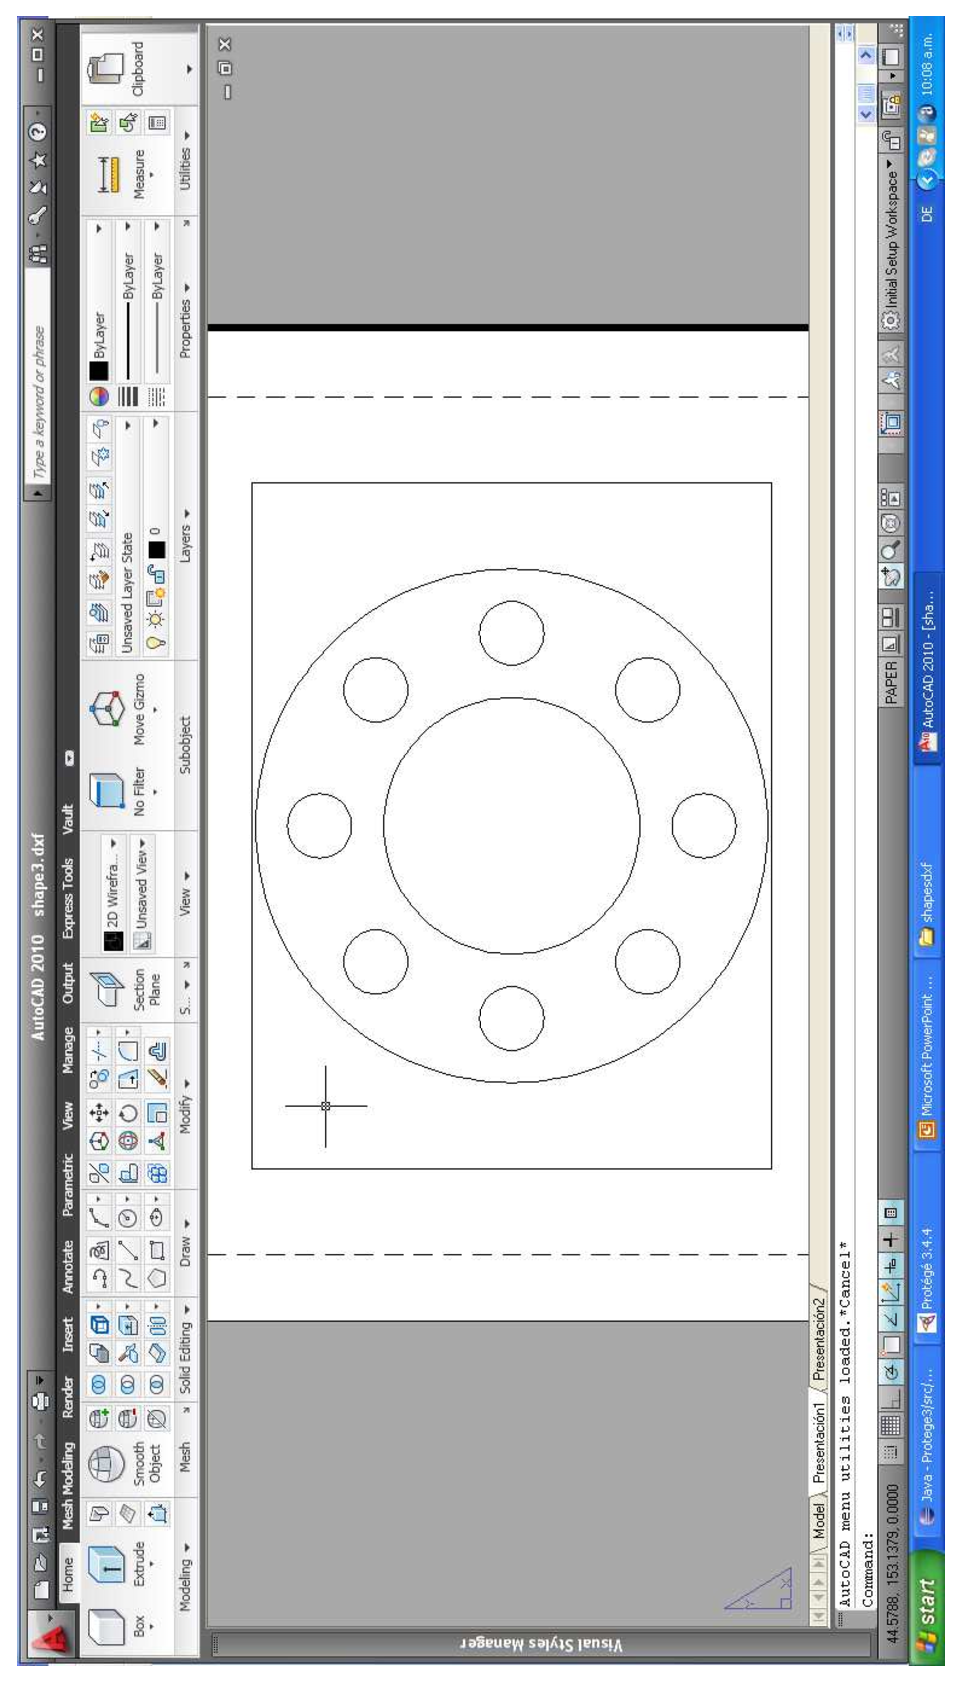
\includegraphics[scale=0.5, angle=270]{figure-chapterIV/fig4-31}\\
	\caption{Shape in AutoCAD}
	\label{figure4-31}
\end{center}
\end{figure}





\begin{figure}
\begin{center}
	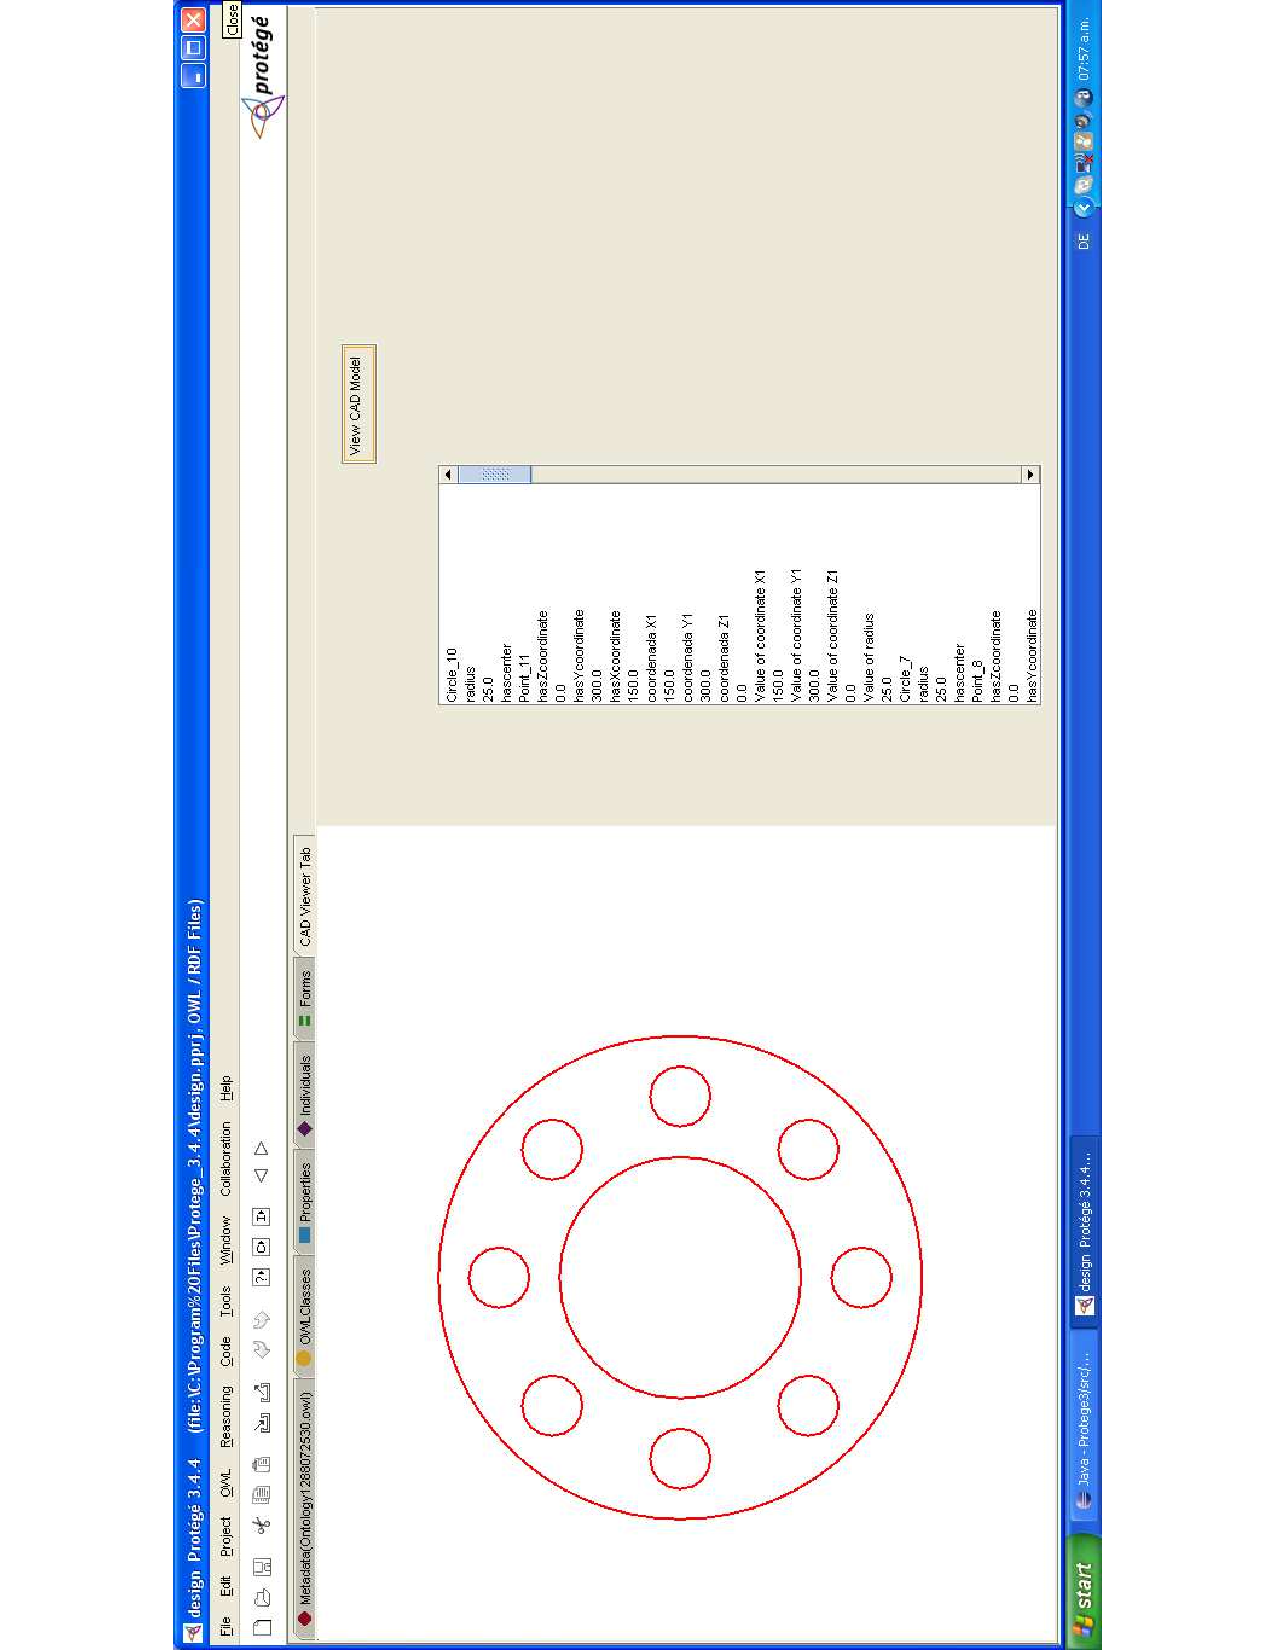
\includegraphics[scale=0.5,angle=270]{figure-chapterIV/fig432}\\
	\caption{Shape in OntoCAD}
	\label{figure432}
\end{center}
\end{figure}


In order to recover the designer intent, it is necessary to provide tools or representations to capture the designer’s knowledge. Moreover, it would be appropriate to support the knowledge of the manufacturing engineer, quality control, and other related tasks as well. 

Fig.\ref{figure4-33} illustrates how we consider Semantic Web Technologies should be ordered in a general framework to make the requirements mentioned in the previous paragraph. Going into details, in Fig.\ref{figure4-33} we propose a foundation of the initial architecture.

In the middle of the architecture, we placed Semantic Web technologies for 2D, and a 2D features ontology. Thus, primitives can be interpreted as features, and quality control can be applied to them. At the top of the architecture, Semantic Web technologies adapted for 3D interpretation are included. A GUI was developed in order to allow visualization of the design. Although this framework apparently covers the aforementioned requirements, we want to introduce a more technical example to view detailed limitations of  the OWL  language for representing certain manufacturing scenarios, and to link it to our evaluation and definition of the above hyperontology.


\begin{figure}
\begin{center}
	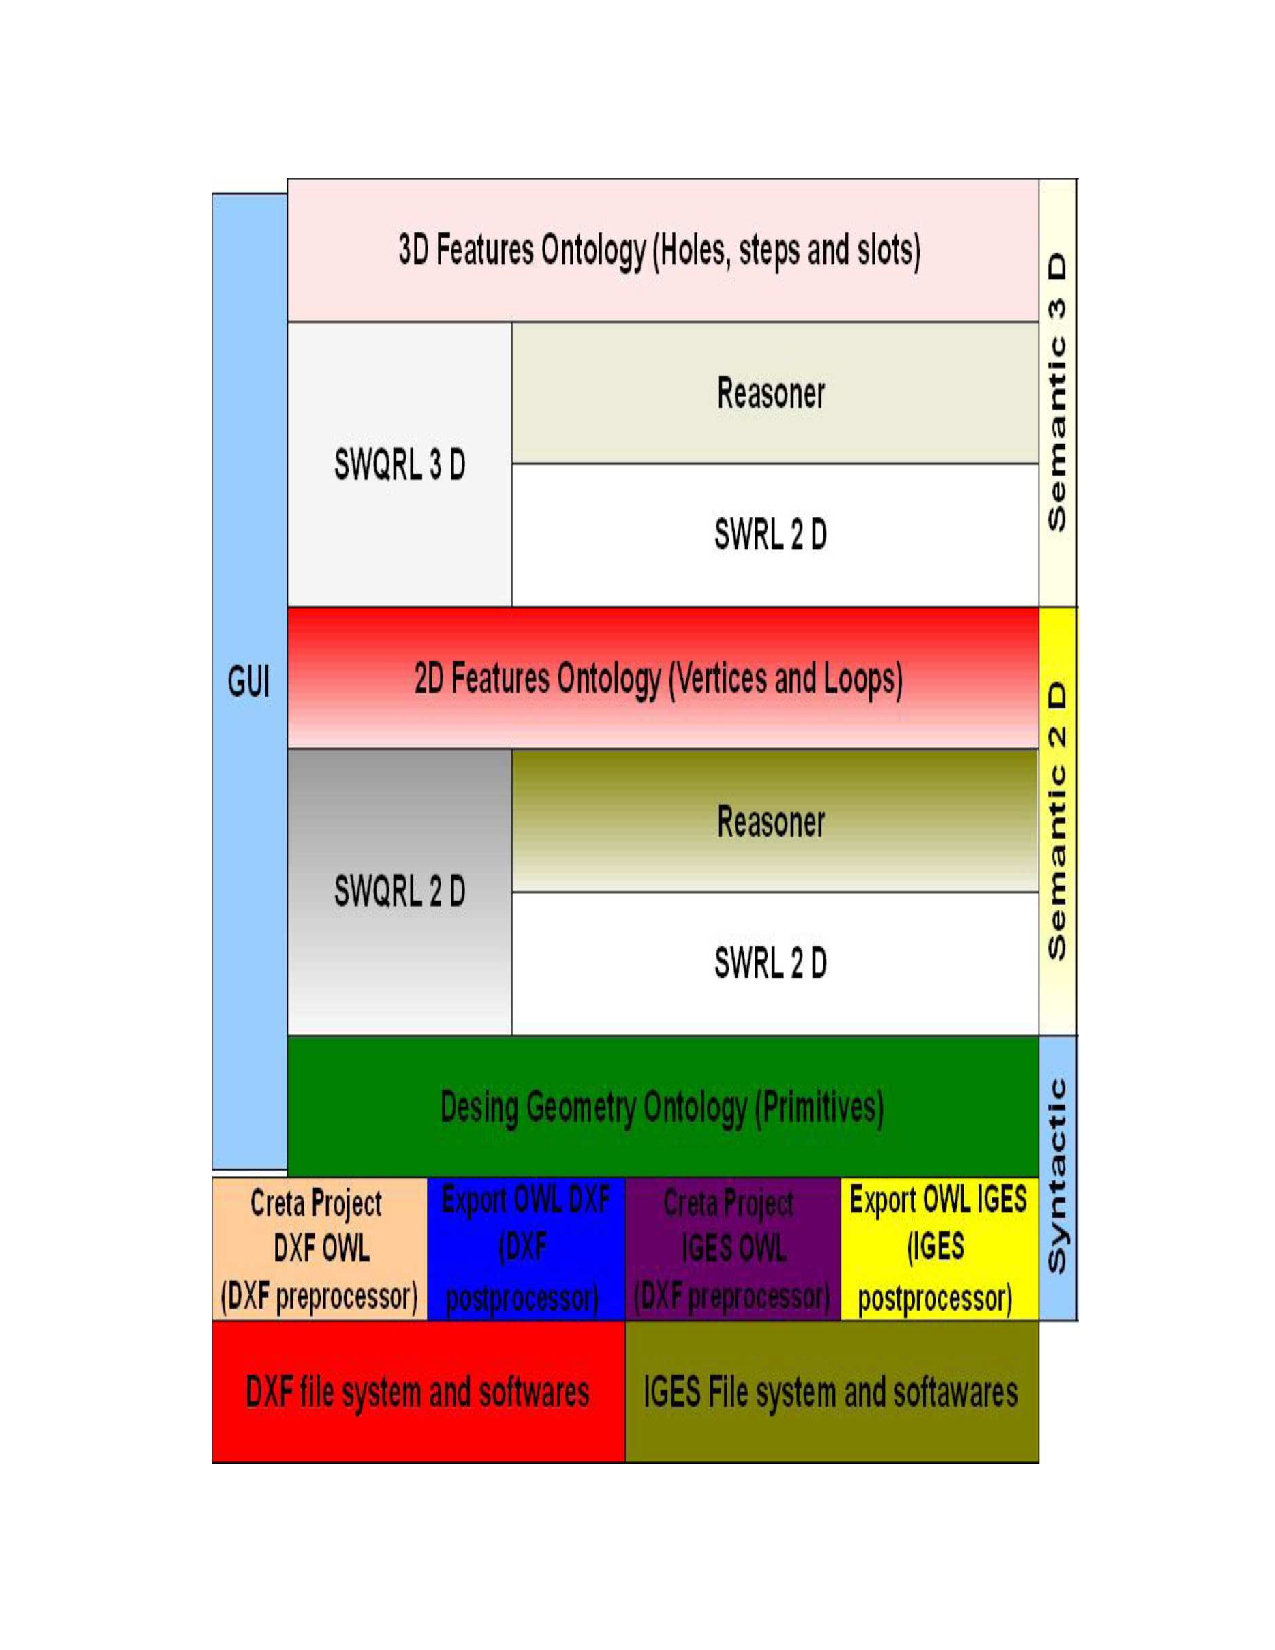
\includegraphics[scale=0.8]{figure-chapterIV/fig4-33}\\
	\vspace{-40}
	\caption{OntoCAD Framework}
	\label{figure4-33}
\end{center}
\end{figure}

As we mentioned in the previous paragraph, we want to introduce a more technical example from the manufacturing point of view, in order to require the major expressivity of OWL. Such an expressivity level demand can be found even in the manufacturing process of 2D design. Sheet   metal parts are some of these. These elements are commonly used in several products manufactured in modern industry: aerospace, automotive, appliances, machine tools, etc. are only some of these. Although various software tools are available for making digital designs for such metal parts, trying to use those designs as input for process planning and manufacturing is not simple.  The majority of standards for Computer Aided Design (CAD) do not represent the particular features required when manufacturing. For instance, declaring when a circle corresponds to an inner edge or an outer edge has significant consequences during manufacturing, although this may not be necessary when displaying designs. Allowing interoperability across the CAD-CAM (Computer Aided Manufacturing) process should enable designers to select optimal manufacturing conditions. For instance, to choose a sheet thickness that would prevent crashes when punching holes.


In order to achieve such interoperability, and according to what we have set out in Section \ref{section2.1} of Chapter \ref{chapter2}, and in Section \ref{section4.3}, manufacturing features must be extracted from CAD files.  Extracting these features demands identifying certain patterns in the CAD files that shall receive additional manufacturing-relevant enrichment.  Information about features is further used to determine the machining tools and manufacturing processes required to manufacture a given design \citep{cayiroglu_new_2009}. Feature information can also then be used to pre-check designs in order to detect production rule violations. If these violations are not detected in an early stage of design, the life cycle of development increases, raising production costs and time to market \citep{radhakrishnan_design_1996}. Manual recognition of the targeted features is not a viable alternative, however: Automated Features Recognition (AFR) is required. However, even nowadays AFR is not fully integrated with CAD software tools. It is applicable only to parts with relatively simple geometry and still requires human intervention to obtain the features identified. Moreover, such techniques are generally supported only in expensive CAD software tools that are beyond the reach of small scale industry \citep{kumar_trends_2005}. 


In \cite{ramos_ontology-based_2011}   we proposed the partial application of the framework presented in Fig. \ref{figure4-33} in order to deal with the shortcomings of AFR from sheet metal designs and designs checking. This ontology-based framework should facilitate interoperability across the entire CAD-CAM process. Our system integrates both a CAD and a features ontology; these ontologies were written in OWL (Web Ontology Language) and represent 2D primitives as lines, arcs and circles in the CAD ontology and as edges, slots, tab and holes in the features ontology. In order to provide rules and query support, OWL was complemented with SWRL and SQWRL. The result is an ontology-based system that allows us to automatically extract the most common manufacturing features referred to in the literature.


One of the main issues of AFR is the abstraction level involved in the manufacturing domain \citep{shah_functional_1988}. On the one hand, designers make designs from the functionality and usability point of view, with its own restrictions and rules. On the other hand, manufacturing engineers evaluate a design from the manufacturing point of view, considering factory constraints. This is mainly the reason why quite distinct standards, formats and tools have been developed. In the two domains, two different interpretations of the requirements take place for the same purpose, so an interoperability channel between them is needed.  This channel needs to enable the interchange of information of products as well as the evaluation of designing and manufacturing restrictions. 

In Fig. \ref{figure4-34}, we introduce the mapping architecture implemented for dealing with this situation. Knowledge transfer between domain ontologies was enabled by a third, mapping ontology, which keeps track of the related concepts of both domains. This mapping ontology was developed using the Prompt plug-in \citep{noy_prompt_2003}. This latter architecture can be considered as a simplified and specialized view of Fig. \ref{figure4-28}, where two terminologically similar ontologies, MASON and OntoStep were hypermapped with BeyondStep within a feature’s hypermodule. Terms present in those ontologies are naturally related to the 3 dimensional domain given the relations found by the results obtained from the extraction of the feature’s hyper module, which was described in Section \ref{subsubsection4.2.5.4}. \cbstart We want to remark that the application, based on the architecture depicted in Fig.\ref{figure4-34}, has a limited scope and it was developed as part of our initial experiences, while the hyperontology proposed in Fig.\ref{figure4-28} has a large scope within the manufacturing domain\cbend 

Moreover, Fig. \ref{figure4-34} makes evident how we deal with one of OWL’s shortcomings, which was the OWL limitation in performing inference over inferred knowledge. In other words, if in a given KB we applied certain rules to determine the quality of a design, and we inferred the design or some parts of it are technically correct, the inferred design or its parts cannot be furtherly reused, unless we record them as asserted knowledge into the same KB. 

This OWL issue is also depicted in Fig. \ref{figure4-33} when we try to move upstream through the architecture, given that in the case of DXF only primitives are exported in this format. Thus 2D features can be inferred in a first stage, but if we try to go forward for a 3D inference, it is necessary to recreate an environment to enable reusing the previously inferred knowledge. Such an environment implies mapping between  several ontologies as in the case displayed in Fig. \ref{figure4-34}. 


\begin{figure}
\begin{center}
	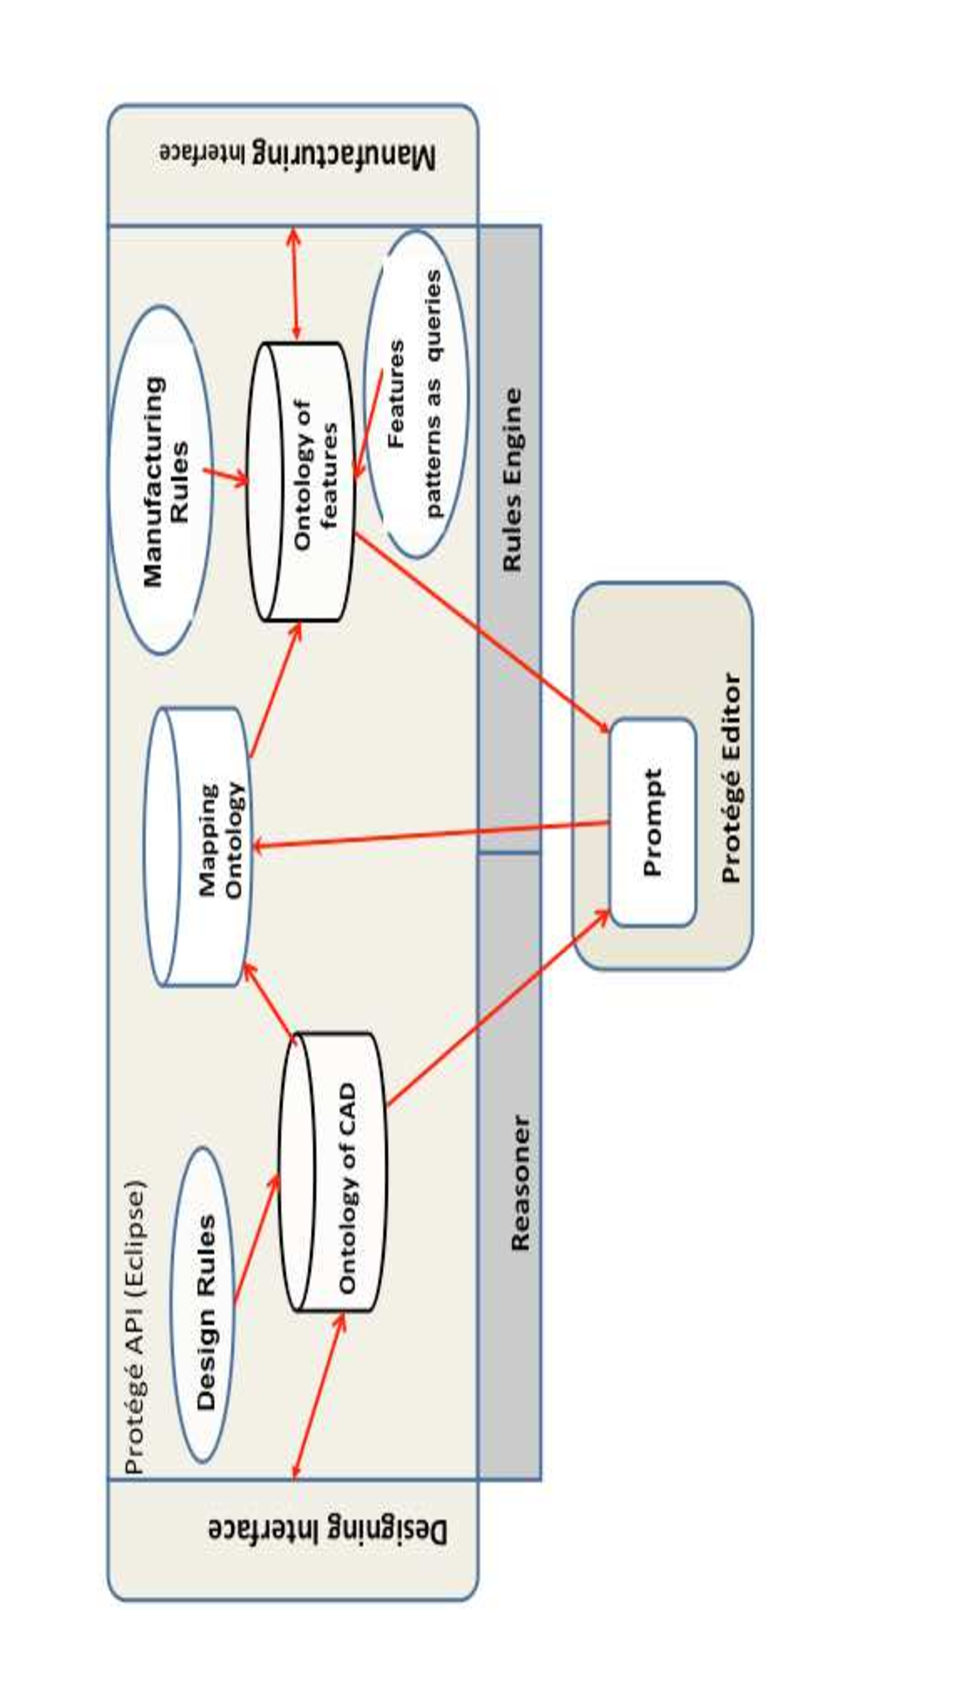
\includegraphics[scale=0.5, angle=270]{figure-chapterIV/fig4-34}\\
	\vspace{-60}
	\caption{Mapping Architecture}
	\label{figure4-34}
\end{center}
\end{figure}


For larger sets of ontologies, and with more complex tasks to perform, we can say that we are in the presence of a hyper-mapped architecture. For instance, manufacturing Operations, mentioned in Fig. \ref{figure4-28}, could be introduced in Fig. \ref{figure4-33} in order to deduce such operations for manufacturing the inferred features. Going into detail, Fig. \ref{figure4-41} lists most of the features mentioned so far, as well as the restrictions required to make them appropriate for manufacturing. Thus, after features are deduced, through the architecture suggested in Fig. \ref{figure4-34} inferred knowledge as features can be available to evaluated  them in order to determine their accuracy with quality restrictions. Every restriction illustrated in Fig. \ref{figure4-35} was successfully represented with OWL, and in all restrictions,    except Distance between holes, quality could be deduced. 



\begin{figure}
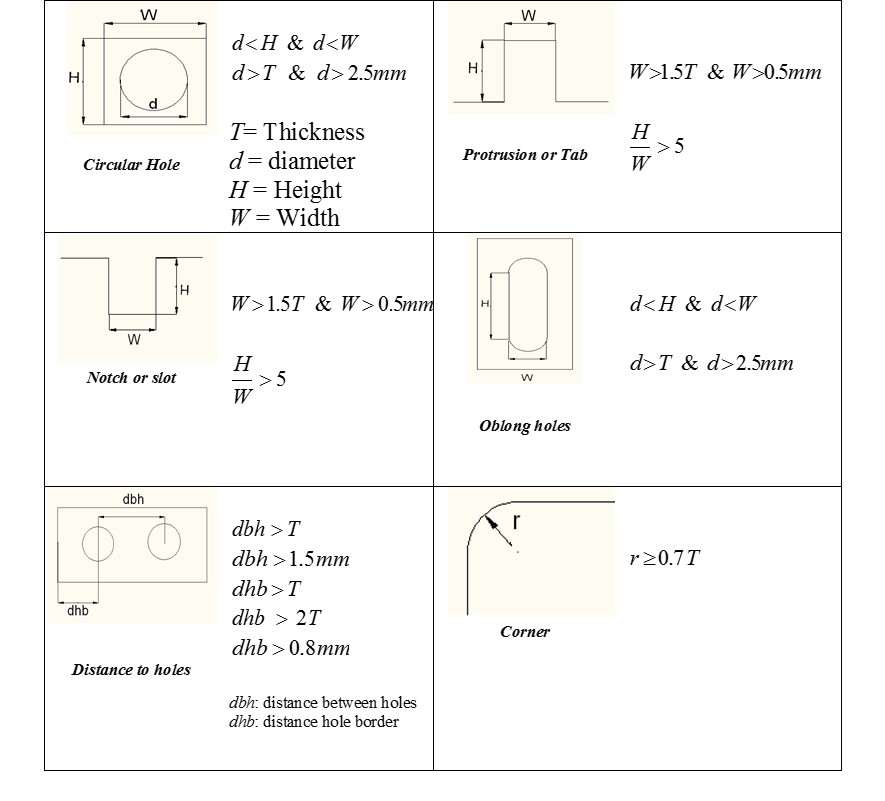
\includegraphics[scale=0.5, angle=-90]{figure-chapterIV/fig4-41}\\
\caption{Manufacturing features with their constraints}
\label{figure4-41}
\end{figure}



\cbstart This last constraint, Distance between  Holes, has a peculiarity. While the others involve binary relations (e.g $has\_Diameter(h_{1},d)$), this one involves a ternary relation (e.g $distance\_Between\_Holes(h_{1},h_{2},d)$), which, as we mentioned in Subsection \ref{subsection2.2.3}, is not possible to be expressed in OWL and is therefore one of the restrictions of this language. In the next section we explain how the heterogeneity approach will help to overcome this issue. \cbend 


\section{Extending Ontologies through Heterogeneity}\label{section4.5}

Given that in the previous section, a shortcoming of OWL was identified during the procedure of trying to represent certain manufacturing rstrictions, and in order to provide inferences for it, it is necessary to recall  Fig. \ref{figure3-1} to determine which course of action to take. In the methodology set out there, a branch toward heterogeneity was included. As we explained in Section \ref{section2.3}, heterogeneity has been proposed as a further way to deal with the limitations of certain logics, making available other logics that provide more reasoning power.


\cbstart In \cite{ramos_hetereogeneous_2012}   we introduced an architecture to deal with the validation of features such as those represented in Fig. \ref{figure4-35}. These in fact correspond to the Distance between holes example mentioned in previous section, and illustrated in Fig. \ref{figure4-41}. That is, there are two holes, $h_{1}$, $h_{2}$, and a restriction of distance $d$ between them . We can represent such a restriction by means of the follwoing ternary relation: $distance\_Between\_Holes(h_{1},h_{2},d)$.  Furthermore, we add a new restriction   called $distance\_Hole\_Border$, which is also mentioned in the literature. These distance features are considered during manufacturing in order to avoid metal deformations when the hole is too close to the border, or when holes are too close to each other as well. \cbend 


\begin{figure}
\begin{center}
	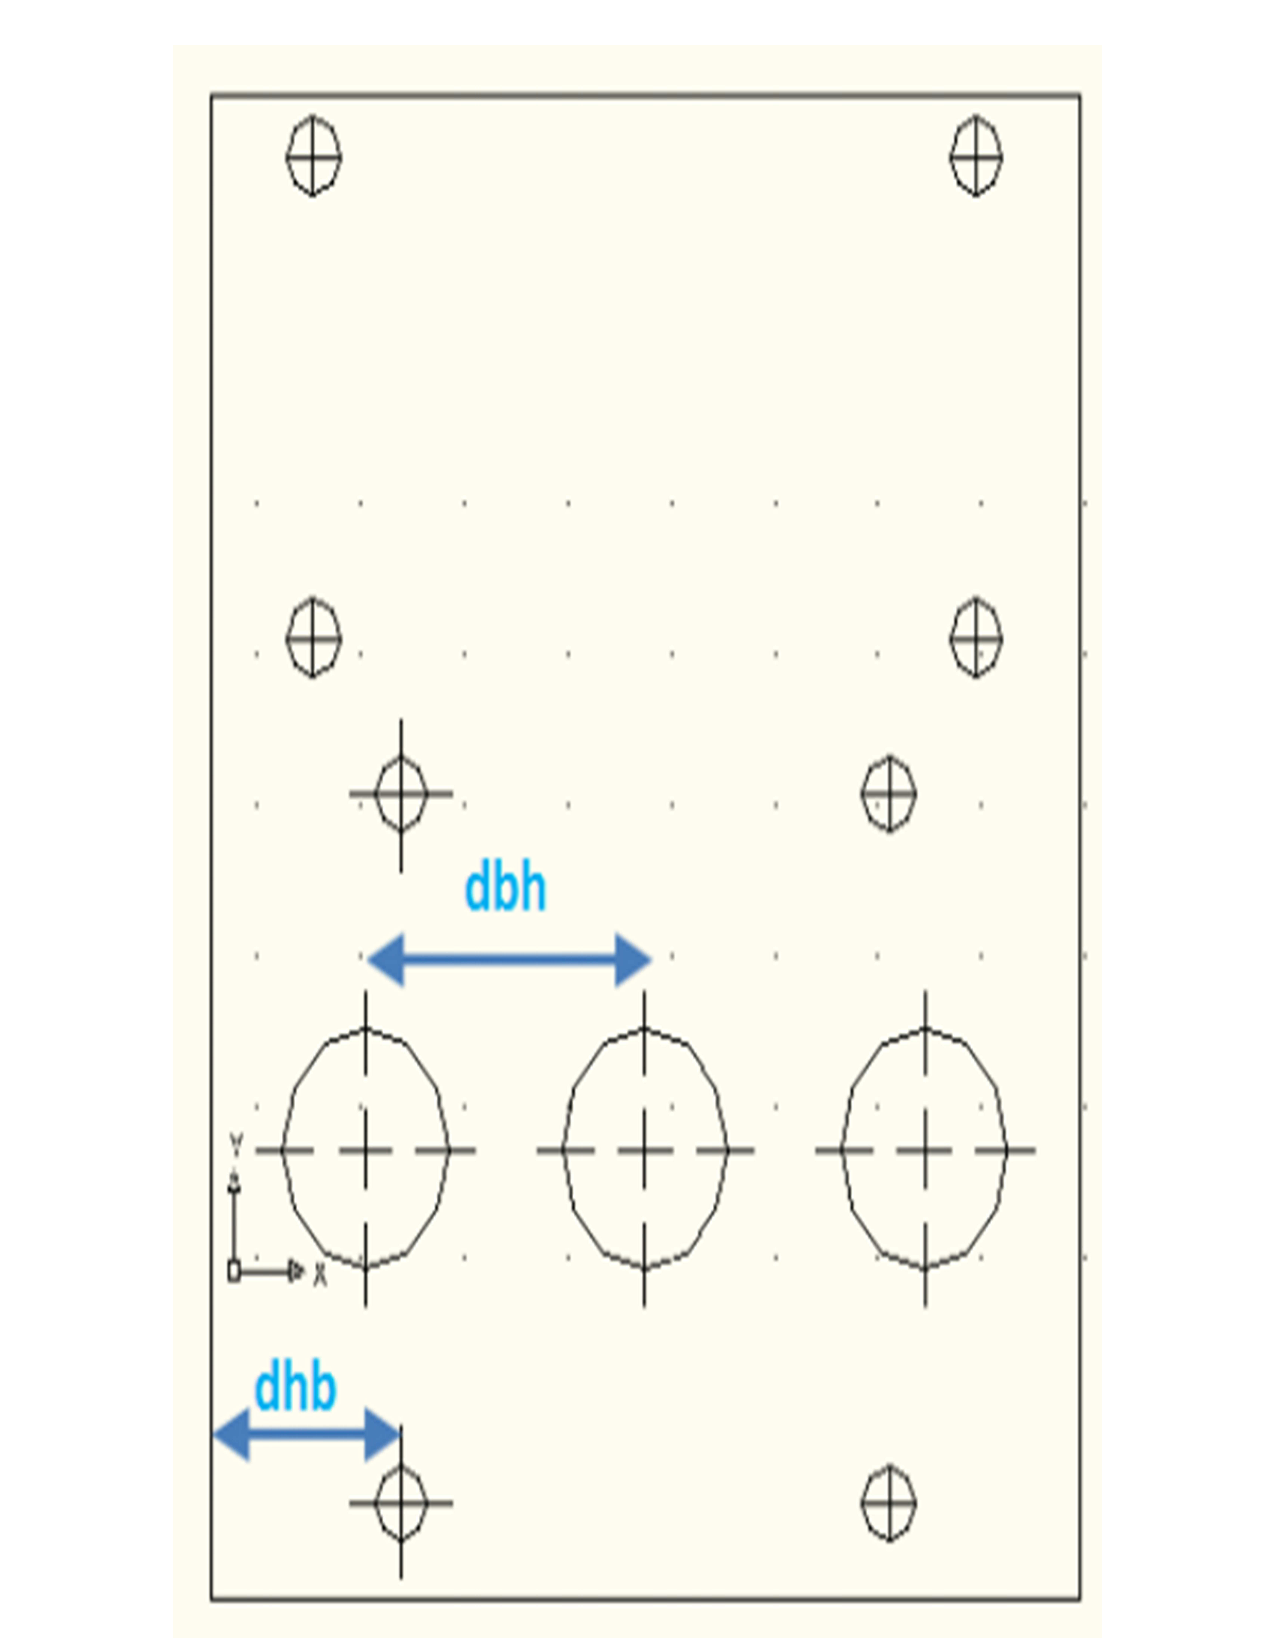
\includegraphics[scale=0.5]{figure-chapterIV/fig4-35}\\
	\caption{Restrictions in Sheet Metal Parts Fabrication  }
	\label{figure4-35}
\end{center}
\end{figure}


Each of these restrictions involves two  instances of the sheet metal issue, and they become related by a valued number restriction. For representing these features, we proceed as follows: in equation \ref{eq4.10}, an intra-feature restriction is present, while in equations \ref{eq4.11} and \ref{eq4.12} inter-feature restrictions are introduced.

\begin{equation}\label{eq4.10}
has\_Diameter(h_{1},d)
\end{equation}

\begin{equation}\label{eq4.11}
distance\_Between\_holes(h_{1}, h_{2}, d)
\end{equation}

\begin{equation}\label{eq4.12}
distance\_Hole\_border(h_{1}, b_{2}, d)
\end{equation}


\cbstart The restriction described in equation \ref{eq4.10} can be represented in OWL and conclusions about the quality of the feature itself can be deduced by reasoning. Restrictions expressed in equations \ref{eq4.11} and \ref{eq4.12} can be indirectly expressed in OWL, but no conclusions about the quality of this design can be obtained from the OWL model because, as we indicated in Section \ref{subsection2.2.3}, and at the end of Section \ref{section4.4}, OWL reasoning is limited to binary relations, while equations \ref{eq4.11} and \ref{eq4.12} illustrate ternary relations \cbend . It is also worth mentioning that the value of these features (dbh and dhb) shown in Fig.\ref{figure4-35} also depend on the materials and other features, for instance thickness. Moreover, we have also avoided mentioning metric units in order to simplify the exposition at this point. This example is an illustration of a type of issue that involves higher predicate arity in a specific task where OWL expressivity is insufficient to reach the validation of certain mechanical features. 


To deal with a scenario such as the one previously described, and to fulfill the modeling requirements of engineering, we at least need an ontology language with a higher expressivity level. But, when we move from OWL to a more expressive ontology language, we also face the risk of falling into undecidable scenarios. This is a common trade off that has been previously studied and for which frameworks have been proposed. In Section \ref{section2.4} those frameworks were presented, and their advantages and restrictions were covered. In this vein, if we can precisely divide the scenarios when OWL is expressive enough for our purposes from the ones where OWL is not enough, then we can introduce a formalism to represent our requirements and evaluate its decidability level.

Therefore, we propose a heterogeneous architecture to bridge the gap between representing and reasoning over manufacturing requirements in the Semantic Web.  Fig. \ref{figure4-36} presents our architecture. It is a modified view of the architecture presented in \cite{w3c_product_2005}. The main difference is  the inclusion of a heterogeneous layer. Such a layer allows us to face engineering requirements written in different logics. Our architecture includes:  

\begin{enumerate}

\item A Product Ontology (PO) that contains product definitions and features that can be represented in a given language and where conclusions concerning their accuracy can also be obtained.  

\item Exemplifications of this PO that can be performed by introducing specific designs into it.  

\item A heterogeneous bridge for when higher expressivity with proof capabilities is required. \textbf{This is expressed in???},  PO bridges with CASL. 

\item Quantities, Units and Scale are also included as elements of this architecture, because they are a fundamental aspect in product descriptions. There are links to the Heterogeneous Bridge because we do not want to employ a fixed standard system, but leave open the possibility of assigning the one preferred by the product user.  

\end{enumerate}



Considering the last mentioned aspect related to unit systems, in this case we decide to validate a library of CAD designs. The features listed in Fig.\ref{figure4-35} could be represented in different metric systems, and even in heterogeneous metric systems (e.g International Metric System, British Metric System). OWL would not be expressive enough for representing and reasoning on the accuracy of such features. Consequently, in order to simplify the scenario we have considered homogeneous designs at this stage, which means a unique homogeneous measurement system. \cbstart HETS and CASL are the basement of our architecture (See Subsection \ref{subsection2.3.2} for a detailed explanation of HETS and CASL). \cbend

Fig. \ref{figure4-37} shows the CASL code corresponding to \texttt{My\_Checker} specification. In the upper part, a Sheet Features Ontology (SFO) is imported with its terminology into My\_Checker, and    the natural numbers library (Nat). Then, a group of ternary predicates are defined: designDistance, standardDistance and properDistance. Finally, we specify that there will be a proper distance if the design distance is greater than the standard distance.

The proof obligation introduced and discussed  in Subsection   \ref{subsection2.3.1} was implemented in \texttt{My\_Checker}. Fig. \ref{figure4-38} introduces this proof obligation for a set of instances from the SFO ontology. There, the \texttt{properDistance} predicate is used to evaluate the values of \texttt{hole\_u1} and \texttt{hole\_u2} from SFO. 


\begin{figure}
\begin{center}
	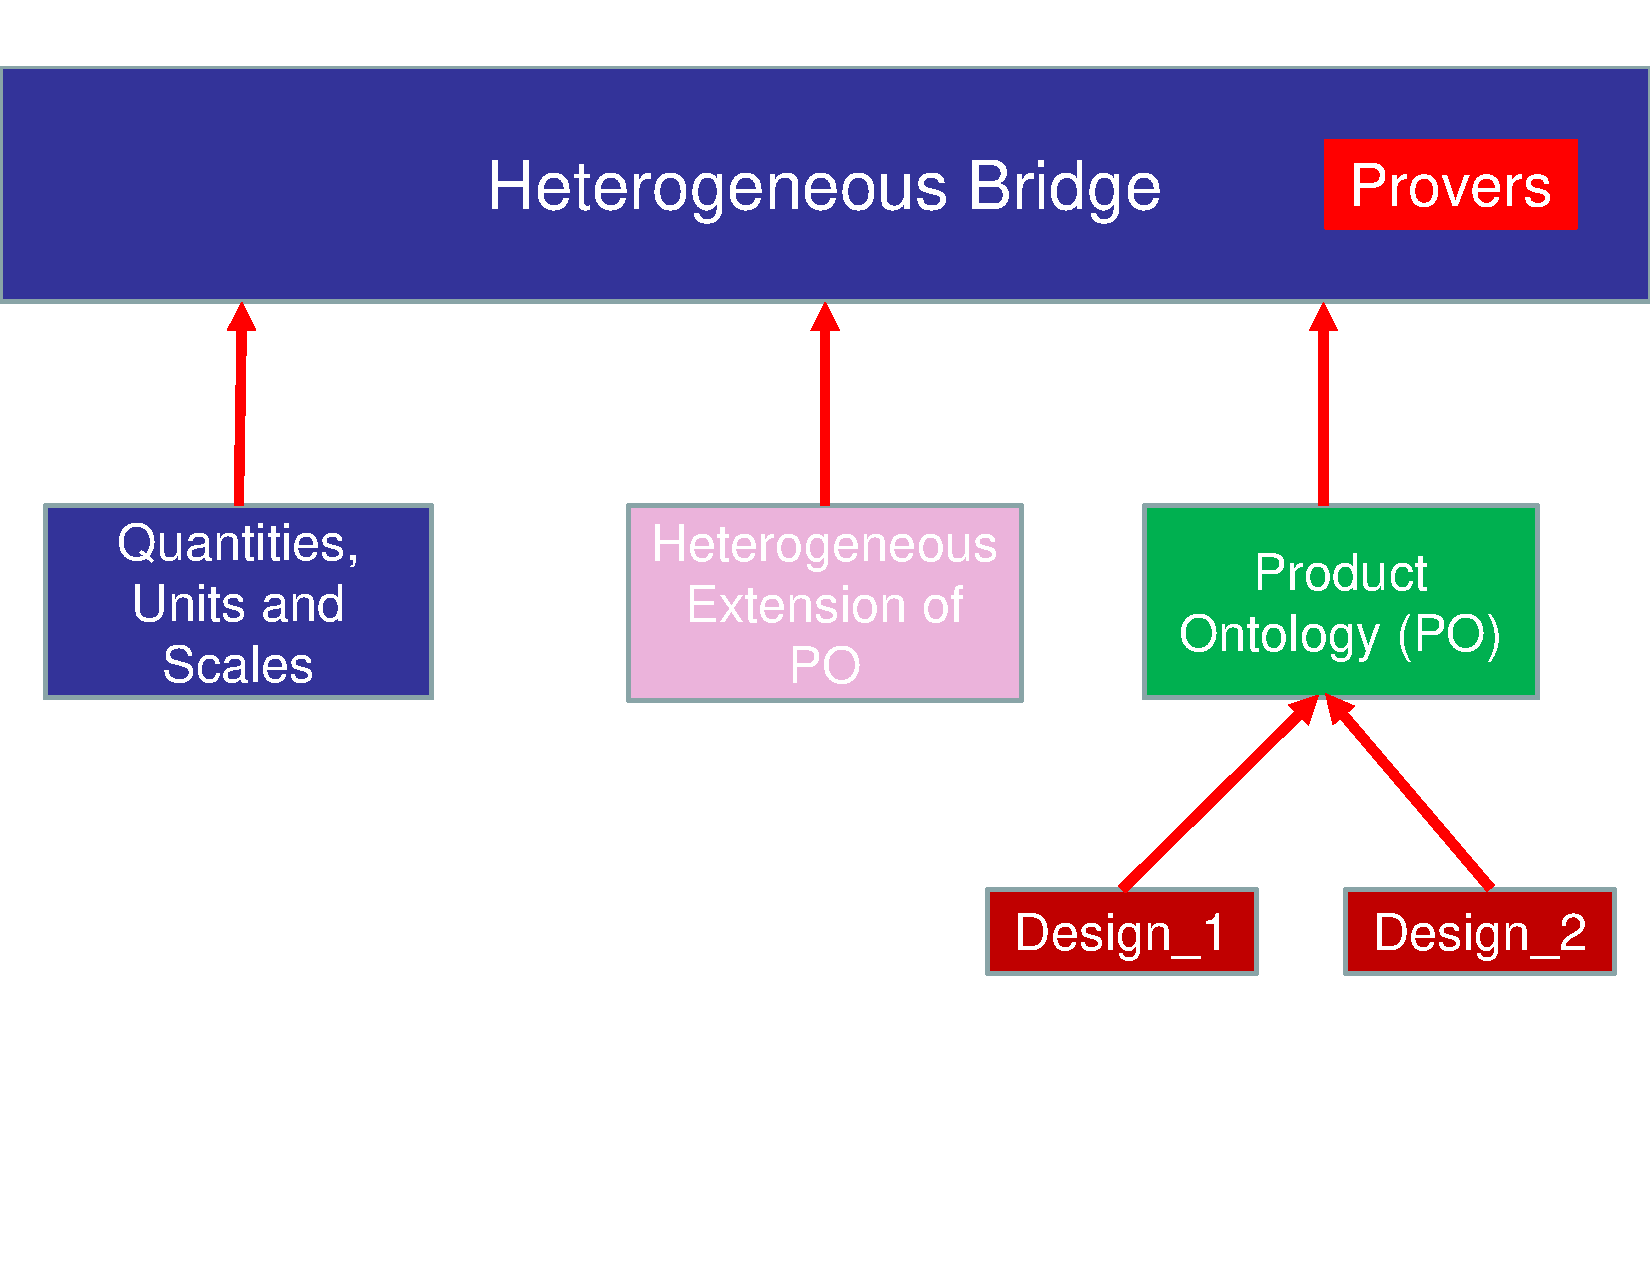
\includegraphics[scale=0.5]{figure-chapterIV/fig4-36.pdf}\\
	\vspace{-40}
	\caption{Heterogeneous Ontological Manufacturing Architecture }
	\label{figure4-36}
\end{center}
\end{figure}



\begin{figure}

\begin{center}
	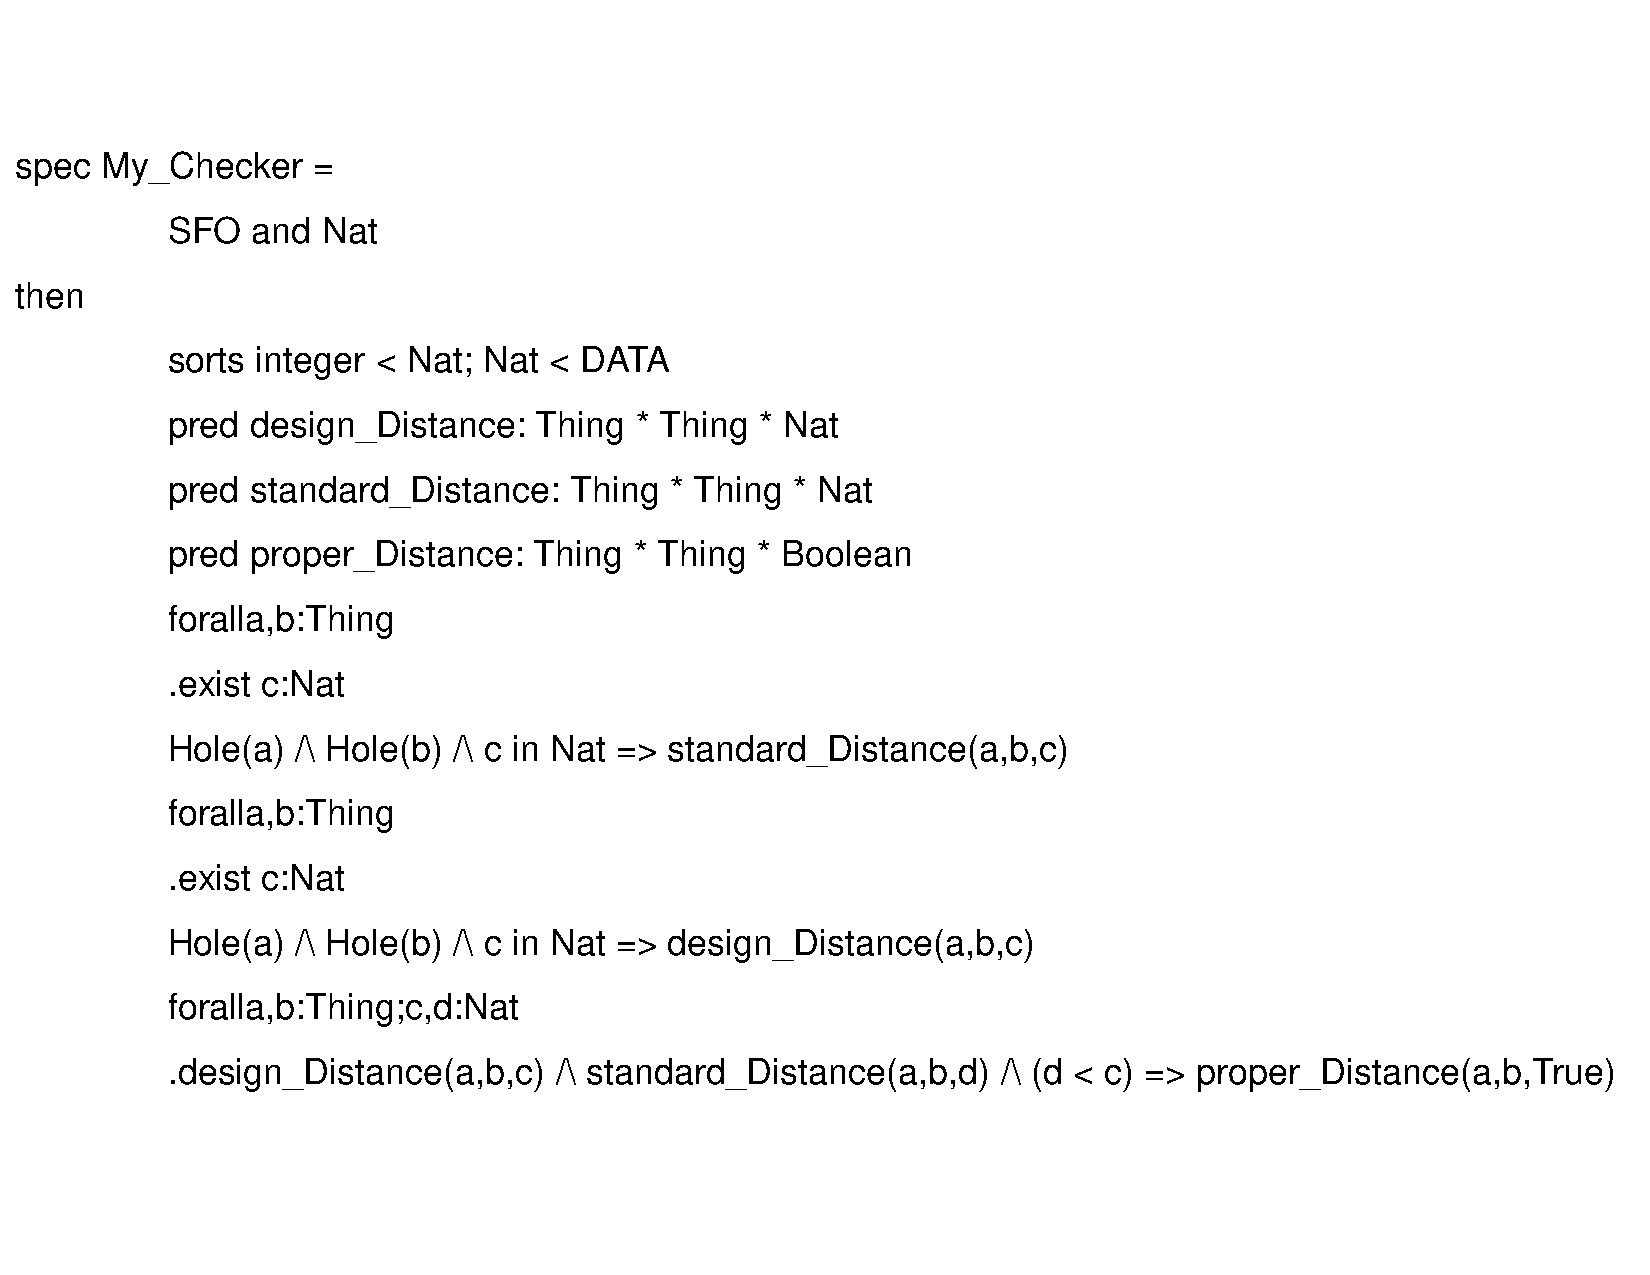
\includegraphics[scale=0.7, angle=90]{figure-chapterIV/fig4-37.pdf}\\
	\caption{Partial View of \texttt{My\_Checker} Spec}
	\label{figure4-37}
\end{center}

\end{figure}


\begin{figure}
\vspace{-50}
\begin{center}
	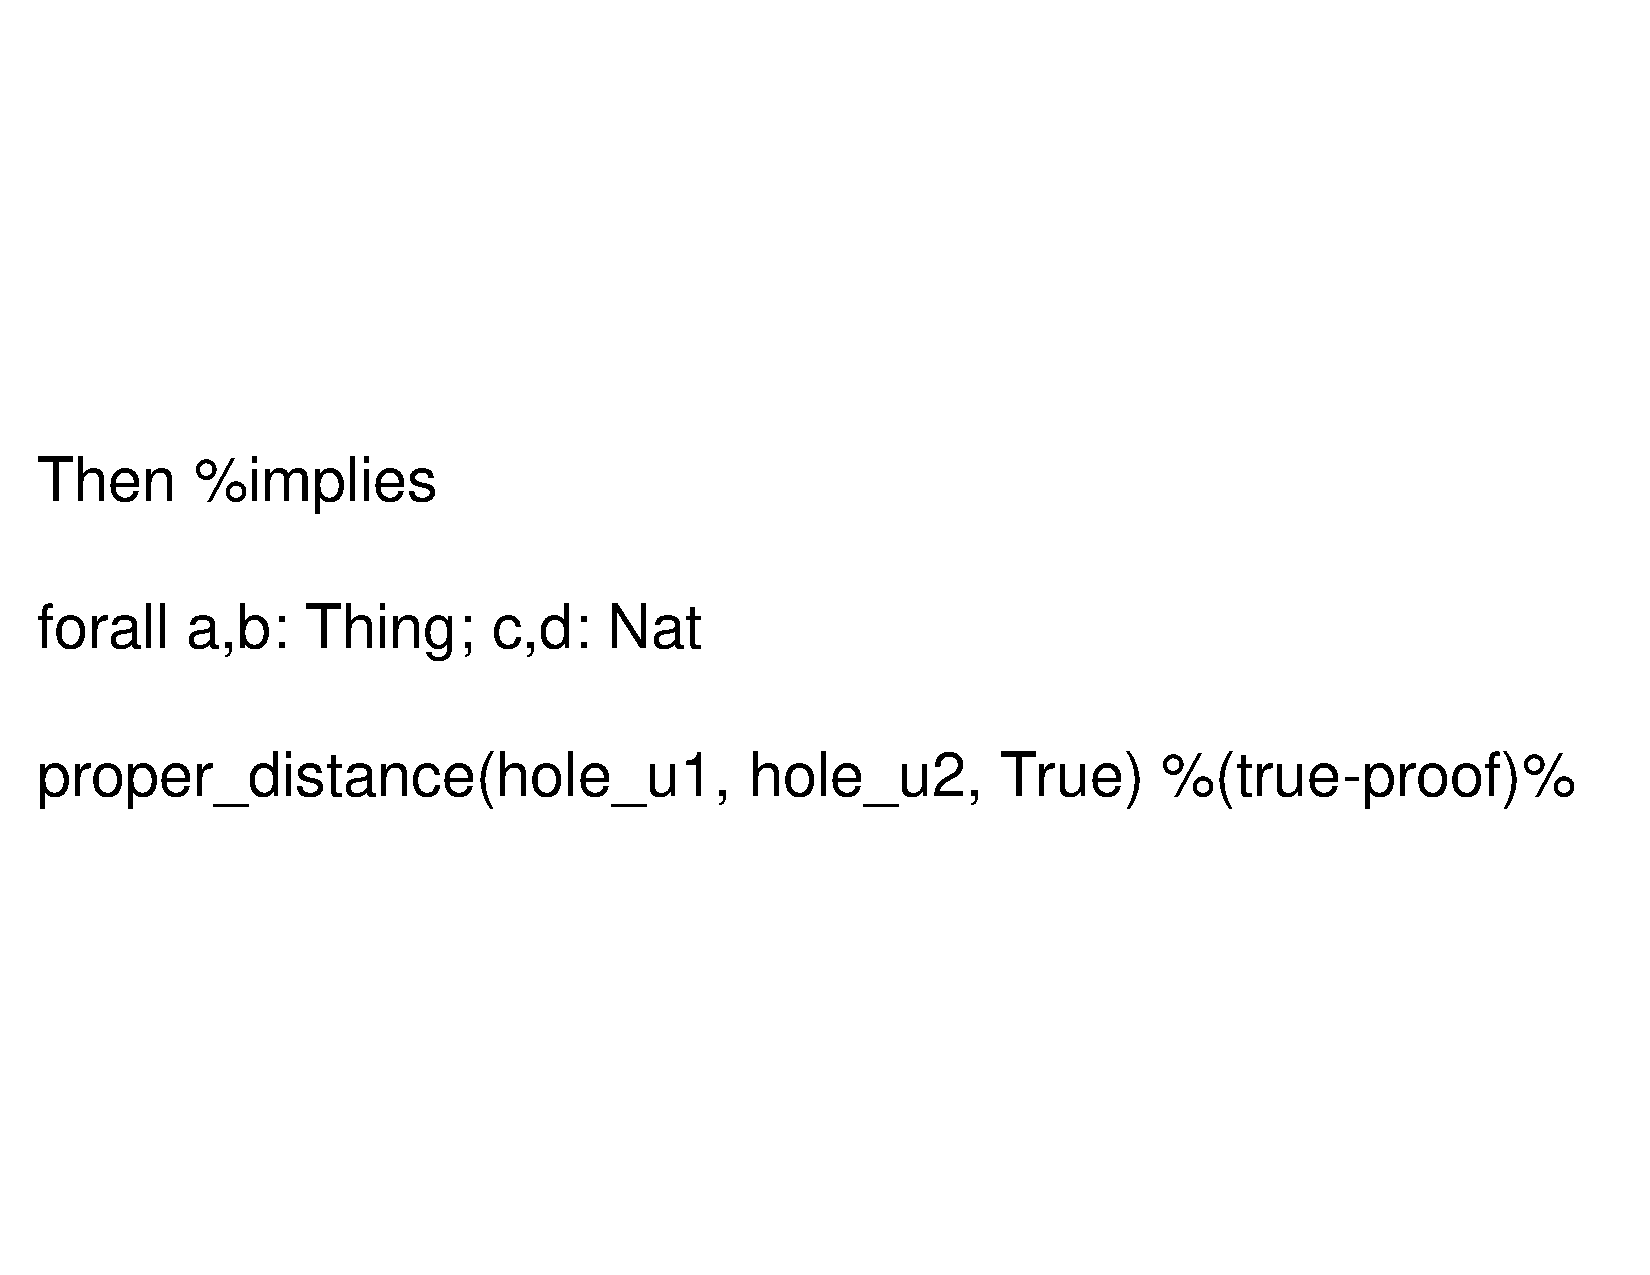
\includegraphics[scale=0.5]{figure-chapterIV/fig4-38.pdf}\\
	\vspace{-80}
	\caption{Instantiated  Proof}
	\label{figure4-38}
\end{center}

\end{figure}



\begin{figure}
\begin{center}
	\includegraphics[scale=0.5, angle=270]{figure-chapterIV/fig4-39}\\
	\caption{\texttt{My\_Checker} HETS view }
	\label{figure4-39}
\end{center}
\end{figure}


After loading the specification in HETS we obtained the windows shown in Fig. \ref{figure4-39}.  On the left side, at the top and bottom, the development graphic is represented. There, nodes named Nat, SFO and \texttt{My\_Checker} correspond to given specifications; such nodes are shown in green color in HETS. More specifically, Nat comes from the library of Numbers (CASL), SFO comes from the SFO (OWL) and \texttt{My\_Checker} imports both (SFO and Nat). The node \texttt{My\_Checker\_E2}, shown in red by HETS, represents proof obligations. On the right side of the same figure, in the top  view we can observe the axiom to be proved representing the proof obligation. Finally, in the  middle of the  window, there is a list of all axioms present in the specification and the available theorem provers. They are identified as “Axioms to Include” and “Theorems to Include if Proven”.  

To complete our task, the theorem prover SPASS \citep{weidenbach_chapter_2001} was run in proof node to assure the correctness of our instantiation. Fig.\ref{figure4-40} depicts the result, which was proved in this opportunity, confirming that our design complies with the technical requirements.



\begin{figure}
\begin{center}
	\includegraphics[scale=0.5, angle=-90]{figure-chapterIV/fig4-40.pdf}\\
	\caption{Proof of Sample provided}
	\label{figure4-40}
\end{center}
\end{figure}

This then overcomes the reasoning OWL restriction, as demonstrated by implementing the architecture proposed in Fig.\ref{figure4-36}.

We have to follow up with the final implementation of the products obtained from the systematic application of the methodology proposed in Fig. \ref{figure3-1}. But in fact, this implementation was carried out progressively from the modularization stage onward. This criterion was captured in our methodology as an \texttt{Implementation} arrow that starts in \texttt{Modularization} and ends in \texttt{Return\_Disp}. \cbstart In other words, since the very beginning a list of competency questions were defined in Subsection \ref{4.1.2}, and since then we followed a course of action in order to provide answer to such questions.\cbend 


Throughout this chapter we captured the implementation of the methodology we proposed in Chapter \ref{chapter3}. Our main motivation for this proposal was the ongoing discussion in ontological engineering which includes topics such as reusability, ULO, modularity and heterogeneity. We proposed some specific metrics and methods to serve as criterion in a development workflow. A group of ontologies related with the manufacturing domain was selected because in this domain, and according to Section \ref{section2.4}, the manufacturing community has shown interest in Ontological Engineering.  These ontologies passed an evaluation procedure, based in information quality and Competency Questions. Given that no ontology provided answers to all competency questions, we tried to make reusable the knowledge encoded in these ontologies. Our first attempt was using one of the ontologies as an interoperability artifact, however according to this proposed metrics and the obtained results, no upper level ontology was found. This result is worth mentioning because some authors have stated that their ontologies were of upper level, and for us these statements can be questions. \cbstart Due to these results it was necessary to continue with our methodological workflow, in order to  fulfill our requirement. Whereby some hyper-modules were extracted from the network ontologies under study. The resulting hyper-modules were integrated in an hyperontology shown in Fig.\ref{figure4-28}. Later, during the implementation phase, the OWL restrictions as ontology language were evidenced to represent the proposed scenario, therefore it was necessary to proceed with the heterogeneous activities proposed in our methodology. The inclusion of an heterogenous layer made possible to complete the workflow, and check the restriction in the product shown in Fig.\ref{figure4-36}. With this result we consider to have complete the methodological workflow we proposed.\cbend


In the next chapter we will represent and discuss our conclusions.  















    
%%    \appendix
%%    \chapter{List of Queries}
  %%  
\label{appendix:a}


\begin{enumerate}
	\item \textbf{get\_businessRegisterNumber}\label{query1}
	\begin{verbatim}
	FOR doc IN egrul_data_collection
	  FILTER doc.businessRegisterNumber.literal !="" 
	  COLLECT WITH COUNT INTO length
	RETURN length
	\end{verbatim}
	
	\item \textbf{get\_taxID}\label{query2}
	\begin{verbatim}
	FOR doc IN egrul_data_collection
	   FILTER doc.taxId.literal !="" 
	   COLLECT WITH COUNT INTO length
	RETURN length
	\end{verbatim}
	
	\item \textbf{get\_informationAboutFounders\_null}\label{query3}
	\begin{verbatim}
	FOR owner in egrul_data_collection
	   FILTER owner.informationAboutFounders == null
	RETURN   owner._id//owner.businessRegisterNumber//
	\end{verbatim}
	
	\item \textbf{get\_informationAboutFounders}\label{query4}
	\begin{verbatim}
	FOR owner in egrul_data_collection
	   FILTER owner.informationAboutFounders != null
	RETURN   owner._id//owner.businessRegisterNumber//
	\end{verbatim}
	
	\item \textbf{get\_informationAboutFounders\_blank}\label{query5}
	\begin{verbatim}
	FOR owner in egrul_data_collection
	   FILTER owner.informationAboutFounders == ""
	RETURN   owner._id//owner.businessRegisterNumber//
	\end{verbatim}
	
	\item \textbf{get\_Owners\_sets}\label{query6}
	\begin{verbatim}
	FOR owner in egrul_data_collection
	    LET InvestmentFund = owner.informationAboutFounders.unitInvestmentFund
	    LET founderIndividual = owner.informationAboutFounders.founderIndividual//
	    LET founder = owner.informationAboutFounders.founder//
	    LET founderForeign = owner.informationAboutFounders.founderForeign
 	  LET founderMunicipalty = owner.informationAboutFounders.founderMunicipalty
 	    
	\end{verbatim}
		\textbf{FILTER  (!( founder != null or founderForeign != null  or founderIndividual != null) 
		or (!(founderMunicipalty != null or InvestmentFund !=null)))}
	\begin{verbatim}
	    LIMIT 100
	    COLLECT WITH COUNT INTO length
	    LIMIT 10
	RETURN length
	
	The FILTER can be changed with some of the following combinations: 
	
	\end{verbatim}
	
	\begin{enumerate}
		
	\item 	((InvestmentFund != null) or (founderIndividual != null)  ) or ((founder == null) or (founderForeign == null) or (founderMunicipalty == null))
	\item 	((founder != null) or (InvestmentFund != null or (founderMunicipalty != null))   ) or ((founderForeign == null) or(founderIndividual == null) )
	\item 	((founderMunicipalty != null) or (founderForeign != null) or (InvestmentFund != null )) or (  (founder == null) or  (founderIndividual == null) )
	\item 	((founderForeign != null) or (InvestmentFund != null )) or (  (founderMunicipalty == null) or (founder == null) or  (founderIndividual == null) )
	\item 	((founderMunicipalty != null) or (InvestmentFund != null )) or ( (founderForeign == null) or (founder == null) or  (founderIndividual == null) )
	\item 	((founderMunicipalty == null) or (founderIndividual != null) or (founder != null)  ) or ( (InvestmentFund == null ) or (founderForeign == null))
	\item 	((founderIndividual != null) or (founder != null)  ) or ( (founderMunicipalty == null) or (InvestmentFund == null ) or (founderForeign == null))
	\item 	((founderIndividual != null) or (founder != null) or (founderForeign != null) ) or ((founderMunicipalty == null) or (InvestmentFund == null ) )
	\item 	((founderMunicipalty != null) or(founderIndividual != null) or (founder != null)  ) or ((InvestmentFund == null ) or (founderForeign == null))
	\item 	((founder != null) or  (founderForeign != null)) or ((founderMunicipalty == null) or (founderIndividual == null) or   (InvestmentFund == null ))
	\item 	((founderMunicipalty != null) or (founder != null)) or ((founderForeign == null) or (founderIndividual == null) or   (InvestmentFund == null ))
	\item 	((founderMunicipalty != null) or (founderForeign != null)) or ((founder == null) or  (founderIndividual == null) or (InvestmentFund == null ))
	\item 	((founderMunicipalty != null)) or ((founderForeign == null) or (founder == null) or  (founderIndividual == null) or (InvestmentFund == null))
	\end{enumerate}

	
	\item \textbf{get\_Ownership\_Relation}\label{query7}
	\begin{verbatim}
	FOR owned in egrul_data_collection
	    filter owned.informationAboutFounders.founder!=null
	    LET founders = owned.informationAboutFounders.founder
	    FILTER LENGTH(founders)  > 0
	    FOR founder IN founders
	        LET OwnerbusinessRegisterNumber = founder.nameAndId.businessRegisterNumber.literal
	        FILTER OwnerbusinessRegisterNumber != null
	        //now we compare with current ownership
	        FOR sanctioned IN ofac_ownership_relation
	            FILTER sanctioned.owned_businessRegisterNumber == OwnerbusinessRegisterNumber
	            LET OwnedbusinessRegisterNumber = owned.businessRegisterNumber.literal
	            LET ownedid = owned._id
	            LET ownerid = CONCAT("egrul_data_collection/",OwnerbusinessRegisterNumber)
	            //writing into collection  with error catch
	            INSERT {_from:ownerid, _to:ownedid,
	            "owned_businessRegisterNumber":OwnedbusinessRegisterNumber} 
	            INTO ofac_ownership_relation // OPTIONS { ignoreErrors: true }
	            	\end{verbatim}
	          \textbf{LIMIT 1100} 
	        	\begin{verbatim}   
	            COLLECT WITH COUNT INTO length
	RETURN  {ownerid, OwnedbusinessRegisterNumber, ownedid}
		            	\end{verbatim}

	\item \textbf{set\_ofac\_100}\label{query8}
	
		\begin{verbatim}
	//set ofac 100 %
	//here we revise every santioned entity belong to only one owner,
	//that this owner owned 100 % of actions, 
	//and that this owner is sanctioned, either by ofac 100, 50 or agg.
	//if that is the case, we proceed to flag them as ofac_sanctioned 100%
	//from the ring 2 we have to confirmed that ofac santioned attribute is not null,
	// I mean we have to confirme previousl company is sanctioned
	//getting id of entity in first collection
	
	FOR doc1 IN ofac_ownership_relation
	   LET doc1id = doc1._to
	   LET ofac_ownerID = doc1._from
	   LET ofac_ownerID2 = LTRIM(ofac_ownerID, "egrul_data_collection/") 
	   LET sanction_value = doc1.ofac_santioned
	   FOR doc2 in egrul_data_collection
	      LET doc2id = doc2._id
	      FILTER doc1id == doc2id
	      //with the company identify, we proceed to coount ownerships if any
	      LET founder = doc2.informationAboutFounders.founder
          LET founder_size = length(founder)
	      LET founderIndividual = doc2.informationAboutFounders.founderIndividual
	      LET founderIndividual_size = length(founderIndividual)
	      LET InvestmentFund = doc2.informationAboutFounders.unitInvestmentFund
	      LET InvestmentFund_size = length(InvestmentFund)
	      LET founderForeign  = doc2.informationAboutFounders.founderForeign
 	      LET founderForeign_size = length(founderForeign)
	      LET founderMunicipalty = doc2.informationAboutFounders.founderMunicipalty
	      LET founderMunicipalty_size = length(founderMunicipalty)
	      //counting total amount of owners
	      LET owners_count = founderIndividual_size+InvestmentFund_size+
	      founderForeign_size+founderMunicipalty_size
	      FILTER (owners_count == 0 and founder_size == 1)
	      FOR doc3 IN founder
	         LET share_size  = doc3.founderShare.sizeOfShares.sizeOfSharePercentage
	         LET ownerID_json = doc3.nameAndId.businessRegisterNumber.literal
	         //here we confirm two conditions:
	         //Owner owns 100 % of the actions
	         //Owner ID is the same in ofac ownership edges 
	         //collection and in egrul main collection. 
	         FILTER (share_size == 100 and ownerID_json == ofac_ownerID2)
	         LET owner_ofac_array = 
	         (
	         FOR doc4 IN ofac_ownership_relation
	            LET doc4id = doc4.owned_businessRegisterNumber
	            //LET doc4id2 = LTRIM(doc4id, "egrul_data_collection/") 
	            FILTER doc4id == ofac_ownerID2//sanctioned owner identified
	            LET ofac_status = doc4.ofac_santioned
	            //FILTER ofac_commited_share != null
	            //COLLECT WITH COUNT INTO length
	            RETURN ofac_status//ofac_commited_share//length
	          )
	      LET owner_ofac_value = owner_ofac_array[0]
	      FILTER owner_ofac_value != null
	      FILTER sanction_value == null
	      UPDATE doc1 WITH {ofac_santioned: "100 %"} IN ofac_ownership_relation//
	      LIMIT 1000
	      COLLECT WITH COUNT INTO length
	RETURN    {doc1id,owner_ofac_value}//,length//
	\end{verbatim}
	
	\item \textbf{set\_ofac\_50}\label{query9}
	\begin{verbatim}
//set ofac 50 %
//here we revise every santioned entity, 
//visit the owners and confirme ownership value is more than or equal to 50 %
//if that is the case, we proceed to flag them as ofac_sanctioned 100%
//getting id of entity in first collection

FOR doc1 IN ofac_ownership_relation//variable to change
   //this is the variable to change across edges
   //this variable chage across set of edges
   LET doc1id = doc1._to//identifier of owned
   LET ofac_ownerID = doc1._from
   LET ofac_ownerID2 = LTRIM(ofac_ownerID, "egrul_data_collection/") 
   LET sanction_value = doc1.ofac_santioned
   FOR doc2 in egrul_data_collection
      LET doc2id = doc2._id
      FILTER doc1id == doc2id
      //with the company identify, we proceed to coount ownership
      LET founder = doc2.informationAboutFounders.founder
      //getting list of founder owners if any
      FILTER founder != null
      //we proceed to identify companies with more than 50 and less than 100 %
      //Note: it is possible than only one company owns less than 100 %, 
      //althought no more owners appear
      FOR doc3 IN founder
         LET share_size  = doc3.founderShare.sizeOfShares.sizeOfSharePercentage
         LET ownerID_json = doc3.nameAndId.businessRegisterNumber.literal
         //here we confirm two conditions:
         //Owner owns 100 % of the actions
         //Owner ID is the same in ofac ownership 
         //edges collection and in egrul main collection. 
         FILTER ((share_size >= 50 and share_size < 100) 
         and ownerID_json == ofac_ownerID2)//
         //checking owner in previous collection is sanctioned
         LET owner_ofac_array = 
         (
            FOR doc4 IN ring4_ofac_ownership_relation//previous owner
               LET doc4id = doc4.owned_businessRegisterNumber
               FILTER doc4id == ofac_ownerID2//sanctioned owner identified
               LET ofac_status = doc4.ofac_santioned
               //COLLECT WITH COUNT INTO length
               RETURN ofac_status//ofac_commited_share//length
            )
         LET owner_ofac_value = owner_ofac_array[0]
         FILTER owner_ofac_value != null
         //filtering owners with exactly one sanctioned flag
         FILTER sanction_value == null
         //after confirming a company is sanctioned, 
         //and owns at least 50 % of a company, we flag it
         UPDATE doc1 WITH {ofac_santioned: "50 %"} IN ofac_ownership_relation
         //variable to change
         LIMIT 1000
         COLLECT WITH COUNT INTO length
RETURN   {share_size, ownerID_json, ofac_ownerID2,   owner_ofac_value} 
	\end{verbatim}
	
    \item \textbf{set\_ofac\_aggregation}\label{query10}
    
	\begin{verbatim}
	
	//set ofac by aggregation from ring 2 
	
	FOR doc1 IN ofac_ownership_relation//this is the variable to change across edges
	//this variable chage across set of edges
	   LET doc1id = doc1._to//identifier of owned
	   LET ofac_ownerID = doc1._from
	   LET ofac_ownerID2 = LTRIM(ofac_ownerID, "egrul_data_collection/") 
	   LET sanction_value = doc1.ofac_santioned//	
	   FOR doc2 in egrul_data_collection
	      LET doc2id = doc2._id
	      FILTER doc1id == doc2id
	      //we confirm we are searching the same owned document
	      //with the company identify, we proceed to coount ownership
	      LET founder = doc2.informationAboutFounders.founder
	      LET founder_size = length(founder)
	      //counting total amount of owners
	      //LET owners_count = founder_size+
	      founderIndividual_size+
	      InvestmentFund_size+
	      founderForeign_size+
	      founderMunicipalty_size
	      FILTER (founder_size > 1)//getting at least one owner
	      //getting size of share in percentage
	      LET ofac_commited_addition = (
	      FOR doc3 IN founder
	         LET share_size  = doc3.founderShare.sizeOfShares.sizeOfSharePercentage
	         FILTER share_size != null
	         LET ownerID_json = doc3.nameAndId.businessRegisterNumber.literal
	         //given that we just know the size of the share for every company, 
	         //we confirm they are sactioned
	         //with a subquery
	            LET owner_ofac_array = 
	            (
	            FOR doc4 IN  ofac_ownership_relation//previous relation link
	               LET doc4id = doc4.owned_businessRegisterNumber
	               FILTER doc4id == ownerID_json//ofac_ownerID2//sanctioned owner identified
	               LET ofac_status = doc4.ofac_santioned
	               FILTER ofac_status != null//here we confirm owner is sanctioned
	            RETURN ofac_status//ofac_commited_share//length
	            )
	         LET owner_ofac = owner_ofac_array[0]
	         FILTER owner_ofac != null
	         //we check there is a sanction flag in owner
	         COLLECT committed_share = share_size
	         RETURN committed_share
	         )//end second subquery
	         LET sum_ofac_shares = SUM(ofac_commited_addition)
	         FILTER sum_ofac_shares >= 50
	         FILTER sanction_value == null//granting that is not previoulsy sanctioned      
	         //with this information we can proceed to flag 
	         UPDATE doc1 WITH {ofac_santioned: "AGG"} IN ofac_ownership_relation//
	RETURN   sum_ofac_shares//
	\end{verbatim}
	
	
	\item \textbf{set\_ofac\_100\_wcs}\label{query11}
	\begin{verbatim}
	
	FOR doc1 IN ofac_ownership_relation
	   LET doc1id = doc1._to//identifier of owned
	   LET ofac_ownerID = doc1._from//identifier of owner
	   LET ofac_ownerID2 = LTRIM(ofac_ownerID, "egrul_data_collection/") 
	   //removing not needed string
	   LET sanction_value = doc1.ofac_santioned//checking if there is previous sanction flag
	      FOR doc2 in egrul_data_collection
	         LET doc2id = doc2._id
	         FILTER doc1id == doc2id
	         LET founder = doc2.informationAboutFounders.founder
 	         LET founder_size = length(founder)
	         LET founderIndividual = doc2.informationAboutFounders.founderIndividual
	         LET founderIndividual_size = length(founderIndividual)
	         LET InvestmentFund = doc2.informationAboutFounders.unitInvestmentFund
	         LET InvestmentFund_size = length(InvestmentFund)
	         LET founderForeign  = doc2.informationAboutFounders.founderForeign
	         LET founderForeign_size = length(founderForeign)
	         LET founderMunicipalty = doc2.informationAboutFounders.founderMunicipalty
	         LET founderMunicipalty_size = length(founderMunicipalty)
	         //counting total amount of owners
	         LET owners_count = founderIndividual_size+
	         InvestmentFund_size+
	         founderForeign_size+
	         founderMunicipalty_size
	         FILTER (owners_count == 0 and founder_size == 1)//getting only one owner, 
	         and that owner has to be founder
	         //getting size of share in percentage
	         FOR doc3 IN founder
	            LET share_size  = doc3.founderShare.sizeOfShares.sizeOfSharePercentage
	            LET ownerID_json = doc3.nameAndId.businessRegisterNumber.literal
	            //here we confirm two conditions:
	            //Owner owns 100 % of the actions
	            //Owner ID is the same in ofac ownership edges collection 
	            //and in egrul main collection. 
	            FILTER (share_size == 100 and ownerID_json == ofac_ownerID2)
	            //we confirm owner id of JSON is in the ownership list
	            //we make a sub query to check if owner has a sanction_value not null, 
	            then we proceed to sanction the child as well
	            //NOTE: in first ring cllection this condition is not fulfilled, 
	            //so we have to ber carefull in his application
	            LET owner_ofac_array = 
	            (
	               FOR doc4 IN ring4_ofac_ownership_relation
	               LET doc4id = doc4.owned_businessRegisterNumber
	               //LET doc4id2 = LTRIM(doc4id, "egrul_data_collection/") 
	               FILTER doc4id == ofac_ownerID2//sanctioned owner identified
	               LET ofac_status = doc4.ofac_santioned
	               RETURN ofac_status//
	               )
	            LET owner_ofac_value = owner_ofac_array[0]
	            FILTER owner_ofac_value != null 
	            FILTER sanction_value == null//here we grant to flag no flagged owned companies
	            UPDATE doc1 WITH {ofac_santioned: "100 %"} IN ofac_ownership_relation//
	            LIMIT 1000
	      COLLECT WITH COUNT INTO length
	RETURN    {doc1id,owner_ofac_value}
	\end{verbatim}
	
		\item \textbf{set\_wcs\_02}\label{query12}
	\begin{verbatim}
	FOR doc1 IN ofac_ownership_relation
	   LET doc1id = doc1._to//identifier of owned
	   LET ofac_ownerID1 = doc1.owner_businessRegisterNumber//identifier of owner
	   LET ofac_ownedID1 = doc1.owned_businessRegisterNumber//identifier of owner
	   LET sanction_value = doc1.ofac_santioned//checking if there is previous sanction flag
	      FOR doc2 in egrul_data_collection
	      LET doc2id = doc2._id
	      FILTER doc1id == doc2id
	      LET businessRegisterNumber = doc2.businessRegisterNumber.literal
	      //with the company identified, we proceed to coount ownerships if any
	      LET founders = doc2.informationAboutFounders.founder
	      LET founder_size = length(founders)
	      LET founderIndividuals = doc2.informationAboutFounders.founderIndividual
	      LET founderIndividual_size = length(founderIndividuals)
	      LET InvestmentFunds = doc2.informationAboutFounders.unitInvestmentFund
	      LET InvestmentFund_size = length(InvestmentFunds)
	      LET foundersForeign  = doc2.informationAboutFounders.founderForeign
	      LET founderForeign_size = length(foundersForeign)
	      LET founderMunicipalties = doc2.informationAboutFounders.founderMunicipalty
	      LET founderMunicipalty_size = length(founderMunicipalties)
	      //counting share per kind of owner
	      //we chek there is at least one founder owner 
	      filter founder_size > 0
	      LET founder_share = (
	         for founder in founders
	         LET share_size  = founder.founderShare.sizeOfShares.sizeOfSharePercentage
	         filter share_size != null
	         COLLECT commited_founder = share_size
	         RETURN commited_founder
	      )
	      LET sum_founder_share = SUM(founder_share)
	      FILTER (sum_founder_share < 50 and sum_founder_share >=0)
	      //giving that company owner have a value less than 50, 
	      //and bigger that 0, then we try ti find an undetermined value of shares
	      //that means a company with declared shares less than 100 %. 
	      //counting shares of individuals
	      LET individual_share = (
	      FILTER founderIndividuals != null
	          for individual in founderIndividuals
	          LET share_individual  = individual.founderShare.sizeOfShares.
	          sizeOfSharePercentage
	          filter share_individual != null
	          COLLECT commited_individual = share_individual
	          RETURN commited_individual
	       )
	      LET sum_individual_share = SUM(individual_share)
	      //counting shares of investment found
	      LET InvestmentFund_share = (
	      FILTER InvestmentFunds != null
	      for InvestmentFund in InvestmentFunds
	         LET share_InvestmentFund  = InvestmentFund.founderShare.sizeOfShares.
	         sizeOfSharePercentage
	         filter share_InvestmentFund != null
	         COLLECT commited_InvestmentFund = share_InvestmentFund
	         RETURN commited_InvestmentFund
	      )
	      LET sum_InvestmentFund_share = SUM(InvestmentFund_share)
	      //counting shares of foundersForeign
	      LET foundersForeign_share = (
	      FILTER foundersForeign != null
	      for founderForeign in foundersForeign
	         LET share_founderForeign  = founderForeign.founderShare.sizeOfShares.
	         sizeOfSharePercentage
	         filter share_founderForeign != null
	         COLLECT commited_foundersForeign = share_founderForeign
	         RETURN commited_foundersForeign
	      )
	      LET sum_foundersForeign_share = SUM(foundersForeign_share)
	     //counting shares of municipality
	      LET founderMunicipalties_share = (
	      FILTER founderMunicipalties != null
	      for founderMunicipalty in founderMunicipalties
	         LET share_founderMunicipalty  = founderMunicipalty.founderShare.sizeOfShares.
	         sizeOfSharePercentage
	         filter share_founderMunicipalty != null
	         COLLECT commited_founderMunicipalty = share_founderMunicipalty
	         RETURN commited_founderMunicipalty
	      )
	      LET sum_founderMunicipalties_share = SUM(founderMunicipalties_share)
	      LET total = sum_founder_share+
	      sum_individual_share+
	      sum_InvestmentFund_share+
	      sum_foundersForeign_share+
	      sum_founderMunicipalties_share
	      FILTER total == 0
	      LET terminated = doc2.informationAboutTermination
	      //check it is not previously sanctioned
	      LET ofac_status_array = 
	      (
	      FOR doc4 IN ofac_ownership_relation//previous relation link
	         LET doc4id = doc4.owned_businessRegisterNumber
	         FILTER businessRegisterNumber == doc4id
	         LET ofac_status = doc4.ofac_santioned
	         RETURN ofac_status//ofac_commited_share//length
	      )
	      LET status_ofac = ofac_status_array[0]
	      filter status_ofac != null//current owner must be sanctioned
	      filter sanction_value == null//current company must not be sanctioned
	      UPDATE doc1 WITH {ofac_santioned: "wcs2"} IN ofac_ownership_relation//
	      LIMIT 10
	RETURN    {status_ofac, total }//
	\end{verbatim}
	
	\item \textbf{set\_wcs\_03}\label{query13}
	\begin{verbatim}
	//set ofac wcs_03
	FOR doc1 IN ofac_ownership_relation
	   LET doc1id = doc1._to//identifier of owned
	   LET ofac_ownerID1 = doc1.owner_businessRegisterNumber//identifier of owner
	   LET ofac_ownedID1 = doc1.owned_businessRegisterNumber//identifier of owner
	   LET sanction_value = doc1.ofac_santioned//checking if there is previous sanction flag
	      FOR doc2 in egrul_data_collection
	      LET doc2id = doc2._id
	      FILTER doc1id == doc2id
	      LET businessRegisterNumber = doc2.businessRegisterNumber.literal
	      //with the company identify, we proceed to coount ownerships if any
	      LET founders = doc2.informationAboutFounders.founder
	      LET founder_size = length(founders)
	      LET founderIndividuals = doc2.informationAboutFounders.founderIndividual
	      //owned id as businessRegisterNumber
	      LET founderIndividual_size = length(founderIndividuals)
	      LET InvestmentFunds = doc2.informationAboutFounders.unitInvestmentFund
	      //owned id as businessRegisterNumber
	      LET InvestmentFund_size = length(InvestmentFunds)
	      LET foundersForeign  = doc2.informationAboutFounders.founderForeign
	      LET founderForeign_size = length(foundersForeign)
	      LET founderMunicipalties = doc2.informationAboutFounders.founderMunicipalty
	      LET founderMunicipalty_size = length(founderMunicipalties)
	      //counting share per kind of owner
	      //we chek there is at least one founder owner 
	      filter founder_size > 0
	      LET founder_share = (
	         for founder in founders
	         LET share_size  = founder.founderShare.sizeOfShares.sizeOfSharePercentage
	         filter share_size != null
	         COLLECT commited_founder = share_size
	         RETURN commited_founder
	      )
	      LET sum_founder_share = SUM(founder_share)
	      FILTER (sum_founder_share < 50 and sum_founder_share >=0)
	      //giving that company owner have a value less than 50, 
	      // and bigger that 0, then we try ti find an undetermined value of shares
	      //that means a company with declared shares less than 100 %. 
	      //counting shares of individuals
	      LET individual_share = (
	      FILTER founderIndividuals != null
	      for individual in founderIndividuals
	         LET share_individual  = individual.founderShare.sizeOfShares.
	         sizeOfSharePercentage
	         filter share_individual != null
	         COLLECT commited_individual = share_individual
	         RETURN commited_individual
	      )
	      LET sum_individual_share = SUM(individual_share)
	      //counting shares of investment found
	      LET InvestmentFund_share = (
	      FILTER InvestmentFunds != null
	      for InvestmentFund in InvestmentFunds
	         LET share_InvestmentFund  = InvestmentFund.founderShare.sizeOfShares.
	         sizeOfSharePercentage
	         filter share_InvestmentFund != null
	         COLLECT commited_InvestmentFund = share_InvestmentFund
	      RETURN commited_InvestmentFund
	      )
	      LET sum_InvestmentFund_share = SUM(InvestmentFund_share)
	      //counting shares of foundersForeign
	      LET foundersForeign_share = (
	      FILTER foundersForeign != null
	      for founderForeign in foundersForeign
	         LET share_founderForeign  = founderForeign.founderShare.sizeOfShares.
	         sizeOfSharePercentage
	         filter share_founderForeign != null
	         COLLECT commited_foundersForeign = share_founderForeign
	         RETURN commited_foundersForeign
	      )
	      LET sum_foundersForeign_share = SUM(foundersForeign_share)
	      //counting shares of municipality
	      LET founderMunicipalties_share = (
	      FILTER founderMunicipalties != null
	      for founderMunicipalty in founderMunicipalties
	         LET share_founderMunicipalty  = founderMunicipalty.founderShare.sizeOfShares.
	         sizeOfSharePercentage
	         filter share_founderMunicipalty != null
	         COLLECT commited_founderMunicipalty = share_founderMunicipalty
	         RETURN commited_founderMunicipalty
	      )
	      LET sum_founderMunicipalties_share = SUM(founderMunicipalties_share)
	      LET total = sum_founder_share+
	      sum_individual_share+
	      sum_InvestmentFund_share+
	      sum_foundersForeign_share+
	      sum_founderMunicipalties_share
	      LET diff = 100 - total
	      LET wcs3 = sum_founder_share + diff
	      FILTER (total < 100 and wcs3 > 50)
	      LET terminated = doc2.informationAboutTermination
	      FILTER terminated == null//if terminated, nothing else to do
	      //check it is not previously sanctioned
	      LET ofac_status_array = 
	      (
	      FOR doc4 IN ring2_ofac_ownership_relation//previous relation link
	         LET doc4id = doc4.owned_businessRegisterNumber
	         FILTER businessRegisterNumber == doc4id
	         LET ofac_status = doc4.ofac_santioned
	         RETURN ofac_status 
	      )
	      LET status_ofac = ofac_status_array[0]
	      FILTER status_ofac != null
	      FILTER sanction_value == null
	UPDATE doc1 WITH {ofac_santioned: "wcs3"} IN ofac_ownership_relation//
	LIMIT 10
	COLLECT WITH COUNT INTO length
	RETURN    length//
	\end{verbatim}
	
	
	
\end{enumerate}



    %%\chapter{Ownership Output}
    %%\label{appendix:b}
\begin{center}
	
	\begin{tabular}{ | c | c |}
		\hline
		\textbf{Collection} & \textbf{Total Ownership} \\ \hline
		Iteration 1 &	875\\ \hline
		Iteration 2 &	883\\ \hline
		Iteration 3 &	339\\ \hline
		Iteration 4 &	215\\ \hline
		Iteration 5 &	275\\ \hline
		Iteration 6 &	237\\ \hline
		Iteration 7 &	281\\ \hline
		Iteration 8 &	205\\ \hline
		Iteration 9 &	149\\ \hline
		Iteration 10 &		204\\ \hline
		Iteration 11 &		199\\ \hline
		Iteration 12 &		156\\ \hline
		Iteration 13 &		239\\ \hline
		Iteration 14 &		187\\ \hline
		Iteration 15 &		151\\ \hline
		Iteration 16 &		209\\ \hline
		Iteration 17 &		192\\ \hline
		Iteration 18 &		150\\ \hline
		Iteration 19 &		235\\ \hline
		Iteration 20 &		181\\ \hline
		Iteration 21 &		151\\ \hline
		Iteration 22 &		224\\ \hline
		Iteration 23 &		210\\ \hline
		Iteration 24 &		148\\ \hline
		Iteration 25 &		234\\ \hline
		
	\end{tabular}
	 \label{table1}
\end{center}






	


    %%\chapter{OFAC Santioned Ownerships}
    %%\input{ofac_table}
    %%\chapter{Worst Case Scenario Results}
    %%\input{wcs_table}
    
   \printglossaries
   
   \bibliography{references3}
\end{document}







